% done

\documentclass[11pt,a4paper,oneside]{book}

\ifdefined\RUSSIAN
\usepackage[english,russian]{babel}
\else
\usepackage[russian,english]{babel}
\fi

\usepackage[T2A]{fontenc}
\usepackage[utf8]{inputenc}
\usepackage{listings}
\usepackage{url}
\usepackage{graphicx}
\usepackage{listingsutf8}
\usepackage[cm]{fullpage}
\usepackage[]{hyperref}
\usepackage{color}
\usepackage{fancyvrb}
\usepackage{xspace}
\usepackage{framed}
\usepackage{ccicons}

\definecolor{lstbgcolor}{rgb}{0.94,0.94,0.94}

\newcommand*{\TT}[1]{\texttt{#1}}
\newcommand*{\IT}[1]{\textit{#1}}
\newcommand*{\EN}[1]{\iflanguage{english}{#1}{}}
\newcommand*{\RU}[1]{\iflanguage{english}{}{#1}}
\newcommand{\LANG}{\RU{ru}\EN{en}}
\newcommand*{\dittoclosing}{---''---}
\newcommand*{\EMDASH}{\RU{ --- }\EN{---}}

\newcommand{\ttf}{\TT{f()}\xspace}
\newcommand{\ttfone}{\TT{f1()}\xspace}

% http://tex.stackexchange.com/questions/32160/new-line-after-paragraph
\newcommand{\myparagraph}[1]{\paragraph{#1}\mbox{}\\} 

\newcommand{\figname}{\RU{илл}\EN{fig}.\xspace}
\newcommand{\figref}[1]{\figname{}\ref{#1}\xspace}
\newcommand{\listingname}{\RU{листинг}\EN{listing}.\xspace}
\newcommand{\lstref}[1]{\listingname{}\ref{#1}\xspace}
\newcommand{\bitENRU}{\RU{бит}\EN{bit}\xspace}
\newcommand{\bitsENRU}{\RU{бита}\EN{bits}\xspace}
\newcommand{\Sourcecode}{\RU{Исходный код}\EN{Source code}\xspace}
\newcommand{\Seealso}{\RU{См. также}\EN{See also}\xspace}
\newcommand{\MacOSX}{Mac OS X\xspace}

% FIXME TODO non-overlapping color!
% \newcommand{\headercolor}{\cellcolor{blue!25}}
\newcommand{\headercolor}{}

\newcommand{\tableheader}{\headercolor{} \RU{смещение}\EN{offset} & \headercolor{} \RU{описание}\EN{description}}

\newcommand{\IDA}{\ac{IDA}\xspace}

\newcommand{\tracer}{\protect\gls{tracer}\xspace}

\newcommand{\Tchar}{\IT{char}\xspace} 
\newcommand{\Tint}{\IT{int}\xspace}
\newcommand{\Tbool}{\IT{bool}\xspace}
\newcommand{\Tfloat}{\IT{float}\xspace}
\newcommand{\Tdouble}{\IT{double}\xspace}
\newcommand{\Tvoid}{\IT{void}\xspace}
\newcommand{\ITthis}{\IT{this}\xspace}

\newcommand{\Ox}{\TT{/Ox}\xspace}
\newcommand{\Obzero}{\TT{/Ob0}\xspace}
\newcommand{\Othree}{\TT{-O3}\xspace}

\newcommand{\oracle}{Oracle RDBMS\xspace}

\newcommand{\idevices}{iPod/iPhone/iPad\xspace}
\newcommand{\olly}{OllyDbg\xspace}

% common C functions
\newcommand{\printf}{\TT{printf()}\xspace} 
\newcommand{\puts}{\TT{puts()}\xspace} 
\newcommand{\main}{\TT{main()}\xspace} 
\newcommand{\qsort}{\TT{qsort()}\xspace} 
\newcommand{\strlen}{\TT{strlen()}\xspace} 
\newcommand{\scanf}{\TT{scanf()}\xspace} 
\newcommand{\rand}{\TT{rand()}\xspace} 

% x86 instructions
\newcommand{\ADD}{\TT{ADD}\xspace} 
\newcommand{\ANDIns}{\TT{AND}\xspace} 
\newcommand{\CALL}{\TT{CALL}\xspace} 
\newcommand{\CPUID}{\TT{CPUID}\xspace} 
\newcommand{\CMP}{\TT{CMP}\xspace} 
\newcommand{\DEC}{\TT{DEC}\xspace} 
\newcommand{\FADDP}{\TT{FADDP}\xspace} 
\newcommand{\FCOM}{\TT{FCOM}\xspace}
\newcommand{\FCOMP}{\TT{FCOMP}\xspace}
\newcommand{\FCOMI}{\TT{FCOMI}\xspace}
\newcommand{\FCOMIP}{\TT{FCOMIP}\xspace}
\newcommand{\FUCOM}{\TT{FUCOM}\xspace}
\newcommand{\FUCOMI}{\TT{FUCOMI}\xspace}
\newcommand{\FUCOMIP}{\TT{FUCOMIP}\xspace}
\newcommand{\FUCOMPP}{\TT{FUCOMPP}\xspace}
\newcommand{\FDIVR}{\TT{FDIVR}\xspace} 
\newcommand{\FDIV}{\TT{FDIV}\xspace} 
\newcommand{\FLD}{\TT{FLD}\xspace} 
\newcommand{\FMUL}{\TT{FMUL}\xspace} 
\newcommand{\FSTP}{\TT{FSTP}\xspace} 
\newcommand{\FDIVP}{\TT{FDIVP}\xspace}
\newcommand{\IDIV}{\TT{IDIV}\xspace} 
\newcommand{\IMUL}{\TT{IMUL}\xspace} 
\newcommand{\INC}{\TT{INC}\xspace} 
\newcommand{\JAE}{\TT{JAE}\xspace} 
\newcommand{\JA}{\TT{JA}\xspace} 
\newcommand{\JBE}{\TT{JBE}\xspace} 
\newcommand{\JB}{\TT{JBE}\xspace} 
\newcommand{\JE}{\TT{JE}\xspace} 
\newcommand{\JGE}{\TT{JGE}\xspace} 
\newcommand{\JG}{\TT{JG}\xspace} 
\newcommand{\JLE}{\TT{JLE}\xspace} 
\newcommand{\JL}{\TT{JL}\xspace} 
\newcommand{\JMP}{\TT{JMP}\xspace} 
\newcommand{\JNE}{\TT{JNE}\xspace} 
\newcommand{\JNZ}{\TT{JNZ}\xspace} 
\newcommand{\JNA}{\TT{JNA}\xspace} 
\newcommand{\JNAE}{\TT{JNAE}\xspace} 
\newcommand{\JNB}{\TT{JNB}\xspace} 
\newcommand{\JNBE}{\TT{JNBE}\xspace} 
\newcommand{\JZ}{\TT{JZ}\xspace} 
\newcommand{\JP}{\TT{JP}\xspace} 
\newcommand{\Jcc}{\TT{Jcc}\xspace} 
\newcommand{\SETcc}{\TT{SETcc}\xspace} 
\newcommand{\LEA}{\TT{LEA}\xspace} 
\newcommand{\LOOP}{\TT{LOOP}\xspace}
\newcommand{\MOVSX}{\TT{MOVSX}\xspace} 
\newcommand{\MOVZX}{\TT{MOVZX}\xspace} 
\newcommand{\MOV}{\TT{MOV}\xspace} 
\newcommand{\NOP}{\TT{NOP}\xspace} 
\newcommand{\POP}{\TT{POP}\xspace} 
\newcommand{\PUSH}{\TT{PUSH}\xspace} 
\newcommand{\NOT}{\TT{NOT}\xspace} 
\newcommand{\RET}{\TT{RET}\xspace} 
\newcommand{\RETN}{\TT{RETN}\xspace} 
\newcommand{\SETNZ}{\TT{SETNZ}\xspace} 
\newcommand{\SETBE}{\TT{SETBE}\xspace} 
\newcommand{\SETNBE}{\TT{SETNBE}\xspace} 
\newcommand{\SUB}{\TT{SUB}\xspace} 
\newcommand{\TEST}{\TT{TEST}\xspace} 
\newcommand{\FNSTSW}{\TT{FNSTSW}\xspace}
\newcommand{\SAHF}{\TT{SAHF}\xspace}
\newcommand{\XOR}{\TT{XOR}\xspace} 
\newcommand{\OR}{\TT{OR}\xspace} 
\newcommand{\SHL}{\TT{SHL}\xspace} 
\newcommand{\SHR}{\TT{SHR}\xspace} 
\newcommand{\LEAVE}{\TT{LEAVE}\xspace} 
\newcommand{\MOVDQA}{\TT{MOVDQA}\xspace} 
\newcommand{\MOVDQU}{\TT{MOVDQU}\xspace} 
\newcommand{\PADDD}{\TT{PADDD}\xspace} 
\newcommand{\PCMPEQB}{\TT{PCMPEQB}\xspace} 

% x86 flags

\newcommand{\ZF}{\TT{ZF}\xspace} 
\newcommand{\CF}{\TT{CF}\xspace} 
\newcommand{\PF}{\TT{PF}\xspace} 

% x86 registers

\newcommand{\AL}{\TT{AL}\xspace} 
\newcommand{\AH}{\TT{AH}\xspace} 
\newcommand{\AX}{\TT{AX}\xspace} 
\newcommand{\EAX}{\TT{EAX}\xspace} 
\newcommand{\EBX}{\TT{EBX}\xspace} 
\newcommand{\ECX}{\TT{ECX}\xspace} 
\newcommand{\EDX}{\TT{EDX}\xspace} 
\newcommand{\DL}{\TT{DL}\xspace} 
\newcommand{\ESI}{\TT{ESI}\xspace} 
\newcommand{\EDI}{\TT{EDI}\xspace} 
\newcommand{\EBP}{\TT{EBP}\xspace} 
\newcommand{\ESP}{\TT{ESP}\xspace} 
\newcommand{\RSP}{\TT{RSP}\xspace} 
\newcommand{\EIP}{\TT{EIP}\xspace} 
\newcommand{\RIP}{\TT{RIP}\xspace} 
\newcommand{\RAX}{\TT{RAX}\xspace} 
\newcommand{\RBX}{\TT{RBX}\xspace} 
\newcommand{\RCX}{\TT{RCX}\xspace} 
\newcommand{\RDX}{\TT{RDX}\xspace} 
\newcommand{\RBP}{\TT{RBP}\xspace} 
\newcommand{\RSI}{\TT{RSI}\xspace} 
\newcommand{\RDI}{\TT{RDI}\xspace} 
\newcommand*{\ST}[1]{\TT{ST(#1)}\xspace}
\newcommand*{\XMM}[1]{\TT{XMM#1}\xspace}

% ARM
\newcommand*{\Reg}[1]{\TT{R#1}\xspace}
\newcommand*{\RegX}[1]{\TT{X#1}\xspace}
\newcommand*{\RegW}[1]{\TT{W#1}\xspace}
\newcommand*{\RegD}[1]{\TT{D#1}\xspace}
\newcommand{\ADREQ}{\TT{ADREQ}\xspace}
\newcommand{\ADRNE}{\TT{ADRNE}\xspace}
\newcommand{\BEQ}{\TT{BEQ}\xspace}

% instructions descriptions
\newcommand{\ASRdesc}{\RU{арифметический сдвиг вправо}\EN{arithmetic shift right}}

% x86 registers tables
% TODO: non-overlapping color!
\newcommand{\RegHeader}{
\RU{
 7 \textsuperscript{(номер байта)} &
 6 &
 5 &
 4 &
 3 &
 2 &
 1 &
 0 }
\EN{
 7th \textsuperscript{(byte number)} &
 6th &
 5th &
 4th &
 3rd &
 2nd &
 1st &
 0th}
}

% FIXME навести порядок тут...
\newcommand{\RegTableThree}[5]{
\begin{center}
\begin{tabular}{ | l | l | l | l | l | l | l | l | l |}
\hline
\RegHeader \\
\hline
\multicolumn{8}{ | c | }{#1} \\
\hline
\multicolumn{4}{ | c | }{} & \multicolumn{4}{ c | }{#2} \\
\hline
\multicolumn{6}{ | c | }{} & \multicolumn{2}{ c | }{#3} \\
\hline
\multicolumn{6}{ | c | }{} & #4 & #5 \\
\hline
\end{tabular}
\end{center}
}

\newcommand{\RegTableOne}[5]{\RegTableThree{#1\textsuperscript{x64}}{#2}{#3}{#4}{#5}}

\newcommand{\RegTableTwo}[4]{
\begin{center}
\begin{tabular}{ | l | l | l | l | l | l | l | l | l |}
\hline
\RegHeader \\
\hline
\multicolumn{8}{ | c | }{#1\textsuperscript{x64}} \\
\hline
\multicolumn{4}{ | c | }{} & \multicolumn{4}{ c | }{#2} \\
\hline
\multicolumn{6}{ | c | }{} & \multicolumn{2}{ c | }{#3} \\
\hline
\multicolumn{7}{ | c | }{} & #4\textsuperscript{x64} \\
\hline
\end{tabular}
\end{center}
}

\newcommand{\RegTableFour}[4]{
\begin{center}
\begin{tabular}{ | l | l | l | l | l | l | l | l | l |}
\hline
\RegHeader \\
\hline
\multicolumn{8}{ | c | }{#1} \\
\hline
\multicolumn{4}{ | c | }{} & \multicolumn{4}{ c | }{#2} \\
\hline
\multicolumn{6}{ | c | }{} & \multicolumn{2}{ c | }{#3} \\
\hline
\multicolumn{7}{ | c | }{} & #4 \\
\hline
\end{tabular}
\end{center}
}



\newcommand{\TITLE}{\IFRU{Краткое введение в reverse engineering для начинающих}
{Quick introduction to reverse engineering for beginners}}
\newcommand{\AUTHOR}{\IFRU{Денис Юричев}{Dennis Yurichev}}
\newcommand{\EMAIL}{dennis@yurichev.com}

\hypersetup{
    pdftex,
    colorlinks=true,
    allcolors=blue,
    pdfauthor={\AUTHOR},
    pdftitle={\TITLE}
    }

\selectlanguage{english}
\setcounter{chapter}{1}

\lstset{
    backgroundcolor=\color{lstbgcolor},
    basicstyle=\footnotesize\ttfamily,
    breaklines=true,
    frame=single,
    inputencoding=cp1251,
}
\renewcommand{\ttdefault}{cmtt} % need it here?

\newcommand{\SignedNumbersSectionName}{\IFRU{Представление знака в числах}
{Signed number representations}}

\newcommand{\WorkingWithFloatAsWithStructSubSubSectionName}{\IFRU
{Работа с типом float как со структурой}{Working with the float type as with a structure}}

\begin{document}

\VerbatimFootnotes

\frontmatter

\begin{titlepage}
\begin{center}
\vspace*{\fill}
\LARGE \TITLE

\vspace*{\fill}

\large \AUTHOR

\large \TT{<\EMAIL>}
\vspace*{\fill}
\vfill

\ccbyncnd

\copyright 2013, \AUTHOR. 

\IFRU{Это произведение доступно по лицензии Creative Commons «Attribution-NonCommercial-NoDerivs» 
(«Атрибуция — Некоммерческое использование — Без производных произведений») 3.0 Непортированная. 
Чтобы увидеть копию этой лицензии, посетите}
{This work is licensed under the Creative Commons Attribution-NonCommercial-NoDerivs 3.0 Unported License. 
To view a copy of this license, visit} \url{http://creativecommons.org/licenses/by-nc-nd/3.0/}.

\IFRU{Версия этого текста}{Text version} 0.1 ({\large \today}).   
\end{center}
\end{titlepage}

\tableofcontents
\cleardoublepage

\chapter{\IFRU{Введение}{Preface}}

\IFRU
{Здесь (будет) немного моих заметок о reverse engineering на русском языке для начинающих, 
для тех кто хочет научиться понимать создаваемый \CCpp компиляторами код для x86 (коего, 
практически, больше всего остального) и ARM.}
{Here (will be) some of my notes about reverse engineering in English language for 
those beginners who like to learn to understand x86 (which is a most large mass of 
all executable software in the world) and ARM code created by \CCpp compilers.}

\IFRU{У термина ``reverse engineering'' минимум два популярных значения: 1) исследование скомпилированных
программ; 2) сканирование трехмерной модели для последующего копирования. Настоящий сборник заметок
связан с первым значением}
{There are two popular meaning of ``reverse engineering'' term: 1) research into compiled programs;
scan of 3D model in order to make a copy of it. These notes are related to first meaning.}

% \section{\IFRU{Целевая аудитория}{Target audience}}



\mainmatter

\chapter{\IFRU{Паттерны компиляторов}{Compiler's patterns}}

\IFRU
{Когда я учил Си, а затем Си++, я просто писал небольшие куски кода, компилировал и смотрел что 
получилось на ассемблере, так мне понять было намного проще. Я делал это такое количество раз, 
что связь между кодом на \CCpp и тем что генерирует компилятор вбилась мне в подсознание достаточно 
глубоко, поэтому я могу глядя на код на асме сразу понимать, в общих чертах, что там было написано 
на Си. Возможно это поможет кому-то еще, попробую описать некоторые примеры.}
{When I first learn C and then C++, I was just writing small pieces of code, compiling it and see what 
is producing in assembler, that was an easy way to me. I did it a lot times and relation 
between \CCpp code and what compiler produce was imprinted in my mind so deep so that 
I can quickly understand what was in C code when I look at produced x86 code. 
Perhaps, this method may be helpful for anyone other, so I'll try to describe here some examples.}

% TODO: english/russian version is also present: URL

\section{\HelloWorldSectionName}
\label{sec:helloworld}

\IFRU{Начнем с знаменитого примера из книги}{Let's start with famous example from the book} ``The C programming Language''\footnote{\url{http://en.wikipedia.org/wiki/The_C_Programming_Language}}:

\lstinputlisting{helloworld/1_1.c}

\subsection{x86}

\subsubsection{MSVC}

\IFRU{Компилируем в}{Let's compile it in} MSVC 2010: \TT{cl 1.cpp /Fa1.asm}

\IFRU
{(Ключ /Fa означает сгенерировать листинг на ассемблере)}
{(/Fa option mean generate assembly listing file)}

\begin{lstlisting}
CONST	SEGMENT
$SG3830	DB	'hello, world', 00H
CONST	ENDS
PUBLIC	_main
EXTRN	_printf:PROC
; Function compile flags: /Odtp
_TEXT	SEGMENT
_main	PROC
	push	ebp
	mov	ebp, esp
	push	OFFSET $SG3830
	call	_printf
	add	esp, 4
	xor	eax, eax
	pop	ebp
	ret	0
_main	ENDP
_TEXT	ENDS
\end{lstlisting}

\IFRU{Компилятор сгенерировал файл \TT{1.obj}, который впоследствии будет слинкован линкером в \TT{1.exe}.} 
{Compiler generated \TT{1.obj} file which will be linked into \TT{1.exe}.}

\IFRU{В нашем случае, этот файл состоит из двух сегментов: \TT{CONST} (для данных-констант) и \TT{\_TEXT} (для кода).}
{In our case, the file contain two segments: \TT{CONST} (for data constants) and \TT{\_TEXT} (for code).} 

\IFRU{Строка \TT{``hello, world''} в \CCpp имеет тип \TT{const char*}, однако не имеет имени.}
{The string \TT{``hello, world''} in \CCpp has type \TT{const char*}, however hasn't its own name.}

\IFRU{Но компилятору нужно как-то с ней работать, так что он дает ей внутреннее имя \TT{\$SG3830}.}
{But compiler need to work with this string somehow, so it define internal name \TT{\$SG3830} for it.}

\IFRU{Как видно, строка заканчивается нулевым байтом ~--- это требования стандарта \CCpp насчет строк.}
{As we can see, the string is terminated by zero byte ~--- this is \CCpp standard of strings.}

\IFRU{В сегменте кода \TT{\_TEXT} находится пока только одна функция ~--- \main.}
{In the code segment \TT{\_TEXT} there are only one function so far ~--- \main.}

\IFRU{Функция \main, как и практически все функции, начинается с пролога и заканчивается эпилогом.}
{Function \main starting with prologue code and ending with epilogue code, like almost any function.}

\IFRU{Об этом смотрите подробнее в разделе о прологе и эпилоге функции}
{Read more about it in section about function prolog and epilog}
~\ref{sec:prologepilog}.

\IFRU{Далее следует вызов функции \printf}
{After function prologue we see a function \printf call}: \TT{CALL \_printf}. 

\IFRU
{Перед этим вызовом, адрес строки (или указатель на нее) с нашим приветствием при помощи инструкции \PUSH помещается в стек.}
{Before the call, string address (or pointer to it) containing our greeting is placed into stack with help of \PUSH instruction.}

\IFRU{После того как функция \printf возвращает управление в функцию \main, адрес строки (или указатель на нее) все еще лежит в стеке.}
{When \printf function returning control flow to \main function, string address (or pointer to it) is still in stack.}

\IFRU{Так как он больше не нужен, то указатель стека (регистр \ESP) корректируется.} 
{Because we do not need it anymore, stack pointer (\ESP register) is to be corrected.}

\TT{ADD ESP, 4} \IFRU{означает прибавить 4 к значению в регистре \ESP.}
{mean add 4 to the value in \ESP register.}

\IFRU
{Почему 4? Так как, это 32-битный код, для передачи адреса нужно аккурат 4 байта. В x64-коде это 8 байт.}
{Why 4? Since it is 32-bit code, we need exactly 4 bytes for address passing through the stack. 
It's 8 bytes in x64-code}

\TT{``ADD ESP, 4''} \IFRU{эквивалентно \TT{``POP регистр''}, но без использования какого-либо регистра\footnote{Флаги
процессора, впрочем, модифицируются}.}
{is equivalent to \TT{``POP register''} but without any register usage\footnote{CPU flags, however, modified}.}

\IFRU
{Некоторые компиляторы, например Intel C++ Compiler, в этой же ситуации, могут вместо 
\ADD сгенерировать \TT{POP ECX} (это можно встретить например в коде \oracle{}, им скомпилированном), 
что почти то же самое, только портится значение в регистре \ECX.}
{Some compilers like Intel C++ Compiler, at the same point, could emit \TT{POP ECX} 
instead of \ADD (for example, this can be observed in \oracle{} code, compiled by Intel C++ compiler), 
and this instruction has almost the same effect, but \ECX register contents will be rewritten.}

\IFRU
{Возможно, компилятор применяет \TT{POP ECX} потому что эта инструкция короче (1 байт против 3).}
{Probably, Intel C++ compiler using \TT{POP ECX} because this instruction's opcode is shorter then 
\TT{ADD ESP, x} (1 byte against 3).}

\IFRU{О стеке можно прочитать в соответствующем разделе}{Read more about stack in relevant section}~\ref{sec:stack}.

\IFRU{После вызова \printf, в оригинальном коде на \CCpp указано \TT{return 0} ~--- вернуть 0 
в качестве результата функции \main.} 
{After \printf call, in original \CCpp code was \TT{return 0} ~--- return zero as a \main function result.} 

\IFRU{В сгенерированном коде это обеспечивается инструкцией}
{In the generated code this is implemented by instruction} \TT{XOR EAX, EAX} 

\IFRU
{\XOR, на самом деле, как легко догадаться, ``исключающее ИЛИ''}
{\XOR, in fact, just ``eXclusive OR''}
\footnote{\url{http://en.wikipedia.org/wiki/Exclusive_or}}, 
\IFRU
{но компиляторы часто используют его вместо простого}
{but compilers using it often instead of}
\TT{MOV EAX, 0} ~--- 
\IFRU
{потому что снова опкод короче (2 байта против 5).}
{slightly shorter opcode again (2 bytes against 5).}

\IFRU{Бывает так, что некоторые компиляторы генерируют}{Some compilers emitting} 
\TT{SUB EAX, EAX}, 
\IFRU
{что значит, \IT{отнять значение \EAX от \EAX}, в любом случае это даст 0 в результате.}
{which mean \IT{SUBtract \EAX value from \EAX}, which is in any case will result zero.}

\IFRU{Самая последняя инструкция \RET возвращает управление в вызывающую функцию.
Обычно, это код \CCpp CRT\footnote{C Run-Time Code}, который, в свою очередь, 
вернет управление операционной системе.}
{Last instruction \RET returning control flow to calling function.
Usually, it's \CCpp CRT\footnote{C Run-Time Code} code, which, in turn, 
return control to operation system.}

\subsubsection{GCC}

\IFRU{Теперь скомпилируем то же самое компилятором GCC 4.4.1 в Linux}
{Now let's try to compile the same \CCpp code in GCC 4.4.1 compiler in Linux}: \TT{gcc 1.c -o 1}

\IFRU{Затем при помощи \IDA. посмотрим как создалась функция \main.}
{After, with the \IDA disassembler assistance, let's see how \main function was created.} 

\IFRU{С другой стороны, мы можем посмотреть результат работы GCC при помощи ключа}
{Note: we could also see GCC assembler result applying option} \TT{-S -masm=intel}

\begin{lstlisting}
main            proc near

var_10          = dword ptr -10h

                push    ebp
                mov     ebp, esp
                and     esp, 0FFFFFFF0h
                sub     esp, 10h
                mov     eax, offset aHelloWorld ; "hello, world"
                mov     [esp+10h+var_10], eax
                call    _printf
                mov     eax, 0
                leave
                retn
main            endp
\end{lstlisting}

\IFRU{Почти то же самое. 
Адрес строки ``hello, world'' лежащей в сегменте данных, в начале сохраняется в \EAX, затем записывается в стек.
А еще в прологе функции мы видим \TT{AND ESP, 0FFFFFFF0h} ~--- 
эта инструкция выравнивает значение в \ESP по 16-байтной границе, делая все значения 
в стеке также выровненными по этой границе (процессор более эффективно работает с переменными расположенными
в памяти по адресам кратным 4 или 16)\footnote{\URLWPDA}.}
{Almost the same.
Address of ``hello world'' string (stored in data segment) is saved in \EAX register first, then it stored into stack.
Also, in function prologue we see \TT{AND ESP, 0FFFFFFF0h} ~--- 
this instruction aligning \ESP value on 16-byte border, resulting all values in stack aligned too
(CPU performing better if values it working with are located in memory at addresses aligned by 
4 or 16 byte border)\footnote{\URLWPDA}.}

\TT{SUB ESP, 10h} \IFRU{выделяет в стеке 16 байт, хотя, как будет видно далее, здесь достаточно только 4.}
{allocate 16 bytes in stack, although, as we could see below, only 4 need here.} 

\IFRU{Это происходит потому что количество выделяемого места в локальном стеке тоже выровнено по 
16-байтной границе.}{This is because the size of allocated stack is also aligned on 16-byte border.}

% TODO: rewrite.
\IFRU{Адрес строки (или указатель на строку) затем записывается прямо в стек без помощи инструкции \PUSH.
\IT{var\_10} по совместительству ~--- и локальная переменная и одновременно аргумент для \printf{}. Подробнее об этом будет ниже.}
{String address (or pointer to string) is then writing directly into stack space without \PUSH instruction use.
\IT{var\_10} ~--- is local variable, but also argument for \printf{}. Read below about it.}

\IFRU{Затем вызывается \printf.}{Then \printf function is called.}

\IFRU{В отличие от MSVC, GCC в компиляции без включенной оптимизации генерирует \TT{MOV EAX, 0} вместо 
более короткого опкода.}{Unlike MSVC, GCC while compiling without optimization turned on, 
emitting \TT{MOV EAX, 0} instead of shorter opcode.}

\IFRU{Последняя инструкция \LEAVE ~--- это аналог команд \TT{MOV ESP, EBP} и \TT{POP EBP} ~--- 
то есть возврат указателя стека и регистра \EBP в первоначальное состояние.} 
{The last instruction \LEAVE ~--- is \TT{MOV ESP, EBP} and \TT{POP EBP} instructions pair equivalent ~--- 
in other words, this instruction setting back stack pointer (\ESP) and \EBP register to its initial state.} 

\IFRU{Это необходимо, т.к., в начале функции мы модифицировали регистры \ESP и \EBP (при помощи}
{This is necessary because we modified these register values (\ESP and \EBP) at the function start (executing}
\TT{\MOV EBP, ESP} / \TT{AND ESP, ...}).

\subsection{ARM}
\label{sec:hw_ARM}

\IFRU{Для экспериментов с процессором ARM, я выбрал два компилятора}{For my experiments with ARM CPU I choose two compilers}: \IFRU{популярный в embedded-среде}{popular in embedded area} Keil Release 6/2013 
\IFRU{и среду разработки}{and} Apple Xcode 4.6.3 \IFRU{}{IDE} (\IFRU{с компилятором}{with} LLVM-GCC 4.2 \IFRU{}{compiler}), \IFRU{генерирующую код для ARM-совместимых процессоров и}{producing code for ARM-comptaible processors and} \IFRU{SoC}{SoCs}\footnote{system on chip} \IFRU{в}{in} \idevices, планшетных компьютеров для Windows 8 и Windows RT\footnote{\url{http://en.wikipedia.org/wiki/List_of_Windows_8_and_RT_tablet_devices}} и таких устройствах как Raspberry Pi.

\subsubsection{\NonOptimizingKeil: \IFRU{режим ARM}{ARM mode}}

\IFRU{Для начала, скомпилируем наш пример в Keil}{Let's start by compiling our example in Keil}:

\begin{lstlisting}
armcc.exe --arm --c90 -O0 1.c 
\end{lstlisting}

\IFRU{Компилятор \IT{armcc} генерирует листинг на ассемблере}{\IT{armcc} compiler producing assembler listing}, 
\IFRU{но он содержит некоторые высокоуровневые макросы связанные с ARM}{but it has some high-level ARM-processor related macros}\footnote{
\IFRU{например, он показывает инструкции \PUSH/\POP отсутствующие в режиме ARM}{for example, it shows \PUSH/\POP instructions absent in ARM mode}}, 
\IFRU{а нам важнее увидеть инструкции ``как есть'', так что посмотрим скомпилированный результат в \IDA}{but it's more important for us to see instructions ``as is'', so let's see compiled results in \IDA}.

\begin{lstlisting}
.text:00000000             main
.text:00000000 10 40 2D E9                 STMFD   SP!, {R4,LR}
.text:00000004 1E 0E 8F E2                 ADR     R0, aHelloWorld ; "hello, world"
.text:00000008 15 19 00 EB                 BL      __2printf
.text:0000000C 00 00 A0 E3                 MOV     R0, #0
.text:00000010 10 80 BD E8                 LDMFD   SP!, {R4,PC}

.text:000001EC 68 65 6C 6C+aHelloWorld     DCB "hello, world",0    ; DATA XREF: main+4
\end{lstlisting}

\IFRU{Вот чуть-чуть фактов о процессоре ARM, которые желательно знать}{Here is couple of ARM-related facts we should know in order to proceed}.
\IFRU{Процессор ARM имеет по крайней мере два основных режима: режим ARM и thumb}{ARM processor has at least two major modes: ARM mode and thumb}. 
\IFRU{В первом (ARM) режиме доступны все инструкции и каждая имеет размер 32 бита (или 4 байта)}{In first (ARM) mode all instructions are enabled and each has 32-bit (4 bytes) size}. 
\IFRU{Во втором режиме (thumb) каждая инструкция имеет размер 16 бит (или 2 байта)}{In second (thumb) mode each instruction has 16-bit (or 2 bytes) size}\footnote{\IFRU{Кстати, инструкции фиксированного размера удобны тем, что всегда можно легко узнать адрес предыдущей инструкции, или следующей}{NOTTRANSLATED}}. 
\IFRU{Режим thumb может выглядеть привлекательнее тем, что программа на нем может быть 1) компактнее; 2) эффективнее исполняться на микроконтроллере с 16-битной шиной данных}{Thumb mode may look attractive because program in it may be 1) compact; 2) executing faster on microcontroller having 16-bit memory datapath}. 
\IFRU{Но за всё нужно платить: в режиме thumb куда меньше возможностей процессора, например, возможен доступ только к 8-и регистрам процессора, и чтобы совершить некоторые действия, выполнимые в режиме ARM одной инструкцией, нужны несколько thumb-инструкций}{Nothing come for free of charge, so, in thumb mode there are reduced instruction set, only 8 registers are accessible and one need several thumb instructions for doing some operations when in ARM mode you'll need just one}.
\IFRU{Начиная с ARMv7, имеется также поддержка инструкций thumb-2, это thumb расширенный до поддержки куда большего числа инструкций}{Starting at ARMv7, there are also thumb-2 instructions set present, this is a thumb extended to support much bigger instructions set}.
\IFRU{Программа для процессора ARM может представлять смесь процедур скомпилированных для обоих режимов}{A program for ARM processor may be mix of procedures compiled for both modes}.
\IFRU{Основное количество приложений для \idevices скомпилировано для набора инструкций thumb-2, потому что Xcode
делает так по умолчанию}{Majority of \idevices applications are compiled for thumb-2 instructions set, because Xcode do this by default}.

\IFRU{В вышеприведененном примере можно легко увидеть что каждая инструкция имеет размер 4 байта}{In example we see here we can easily see that each instruction has size of 4 bytes}.
\IFRU{Действительно, ведь мы же компилировали наш код для режима ARM а не thumb}{Indeed, we compiled our code for ARM mode, but for thumb}.

\IFRU{Самая первая инструкция}{The very first instruction} \TT{''STMFD SP!, \{R4,LR\}''}\footnote{Store Multiple Full Descending} \IFRU{работает как инструкция}{works here as} \PUSH, \IFRU{записывает значения двух регистров}{instruction, writing values of two} (\TT{R4} \IFRU{и}{and} \LR) \IFRU{в стек}{registers into stack}. 
\IFRU{Действительно, в выдаваемом листинге на ассемблере, компилятор \IT{armcc}, для упрощения, указывает здесь инструкцию}{Indeed, in output listing, \IT{armcc} compiler, for the sake of simplification, showing here} \TT{''PUSH \{r4,lr\}''}\IFRU{}{instruction}.
\IFRU{Но это не совсем точно, инструкция \PUSH доступна только в режиме thumb, поэтому, во избежания путанницы, я предложил работать в \IDA}{But it's not quite correct, \PUSH instruction available only in thumb mode, so, to make things less messy, I offered to work in \IDA}.

\IFRU{Итак, эта инструкция записывает значения регистров \TT{R4} и \LR по адресу в памяти, на который указывает регистр \SPwithfootnote, затем уменьшает \TT{SP}, чтобы он указывал на место в стеке, доступное для новых записей}{So this instruction writes values of \TT{R4} and \LR registers at the address in memory to which \SPwithfootnote pointing, then decrements \SP so it will points to a place in stack free for new entries}.

\IFRU{Эта инструкция, как и инструкция \PUSH в режиме thumb, может сохранить в стеке одновременно несколько значений регистров, что может быть очень удобно}{This instruction, like \PUSH instruction in thumb mode, is able save several register values at once and this may be useful}. 
\IFRU{Кстати, такого в x86 нет}{By the way, there is no such thing in x86}. 
\IFRU{Так же следует заметить, что \TT{STMFD} ~--- генерализация инструкции \PUSH (то есть, расширяет её возможности), потому что может работать с любым регистром а не только с \SP, это тоже может быть очень удобно}{It's also can be noted that \TT{STMFD} ~--- generalization of \PUSH instruction (extending its features), because it can work with any register, not just with \SP and this can be very useful}.

\IFRU{Инструкция}{} \TT{''ADR R0, aHelloWorld''} \IFRU{прибавляет значение регистра \PC к смещению, где хранится строка}{instruction adding \PC register value to the offset, where the} \IT{``hello, world''} \IFRU{}{string is located}. 
\IFRU{Причем здесь \PC, можно спросить}{How \TT{PC} register used here, one might ask}?
\IFRU{Притом, что это так называемый ``адресно-независимый код''}{This is so called ``position-independent code''}\footnote{\IFRU{Читайте больше об этом в соответствующем разделе}{Read more about it in relevant section}~\ref{sec:PIC}}, \IFRU{он предназначен для исполнения будучи не привязанным к каким-либо адресам в памяти}{it is intended to be executed not to be fixed to any addresses in memory}.
\IFRU{В опкоде инструкции \TT{ADR} указывается разница между адресом этой инструкции и местом, где хранится строка}{In the opcode of \TT{ADR} instruction, here is encoded a difference between address of this instruction and the place where the string is located}.
\IFRU{Эта разница всегда будет постоянной, вне зависимости от того, куда был загружен операционной системой наш код}{Difference will always be constant, without any dependence to the address where that code being loaded, by operation system, presumably}. 
\IFRU{Поэтому всё что нужно это прибавить адрес текущей инструкции (из \PC) чтобы получить текущий абсолютный адрес нашей Си-строки}{That's why all we need is to add address of current instruction (from \PC) in order to get absolute address of our C-string in memory}.

\IFRU{Инструкция}{} \TT{''BL \_\_2printf''}\footnote{Branch with Link} \IFRU{вызывает функцию \printf}{instruction calling \printf function}. 
\IFRU{Работа этой инструкции состоит из двух фаз}{That's how this instruction works}: 
\begin{itemize}
\item
\IFRU{записать адрес после инструкции \TT{BL} (0xC) в регистр \LRwithfootnote}{write address after \TT{BL} instruction (0xC) into \LRwithfootnote register};
\item
\IFRU{затем собственно передать управление в \printf, записав адрес этой функции в регистр \PCwithfootnote}{then pass control flow into \printf by writing its address into \PCwithfootnote register}.
\end{itemize}

\IFRU{Ведь, когда функция \printf закончит работу, нужно знать, куда вернуть управление, поэтому закончив работу, всякая функция передает управление по адресу записанному в регистре \LR}{Because, when \printf finishes its work, it should have information, where it should return control, that's why each function passes control to the address stored in \LR register}.

\IFRU{В этом разница между ``чистыми'' RISC-процессорами вроде ARM и x86, где адрес возврата записывается в стек}{That is the difference between ``pure'' RISC-processors like ARM and x86, where address of return is stored in stack}\footnote{\IFRU{Подробнее об этом будет описано в следующей главе}{Read more about this in next section}~\ref{sec:stack}}.

\IFRU{Кстати, 32-битный абсолютный адрес, либо же смещение, невозможно закодировать в 32-битной инструкции \TT{BL}, в ней есть место только для 24-х бит}{By the way, absolute 32-bit address or offset cannot be encoded in 32-bit \TT{BL} instruction, because it has space only for 24 bits}.
\IFRU{Так же следует отметить, что из-за того что все инструкции в режиме ARM имеют длину 4 байта (32 бита), и инструкции могут находится только по адресам кратным 4, то последние 2 бита (всегда нулевых) можно не кодировать.}{It's also worth to note that all ARM mode instructions has size 4 bytes (32 bits), hence they all can be located only on 4-byte boundary addresses. This mean, last 2 bits of instruction address (always zero bits) may be omitted.}
\IFRU{В итоге имеем 26 бит, при помощи которых можно закодировать смещение}{In summary, we have 26 bit for offset encoding, this is enough to represent offset} $\pm{}\approx{}32M$.

\IFRU{Следующая инструкция}{Next} \TT{''MOV R0, \#0''}\footnote{MOVe} \IFRU{просто записывает 0 в регистр \TT{R0}}{instruction just writes 0 into \TT{R0} register}.
\IFRU{Ведь наша Си-функция возвращает 0 а возвращаемое значение всякая функция оставляет в \TT{R0}}{That's because our C-function returning 0 and returning value is to be placed in \TT{R0}}.

\IFRU{Последняя инструкция}{The last instruction} \TT{''LDMFD SP!, {R4,PC}''}\footnote{Load Multiple Full Descending} \IFRU{это инструкция обратная от}{is an inversive instruction of} \TT{STMFD}, \IFRU{она загружает из стека значения для сохранения их в \TT{R4} и \PC, увеличивая указатель стека \SP}{it loads values from stack for saving them into \TT{R4} and \PC, incremeting stack pointer \SP}.
\IFRU{Это, в каком-то смысле, аналог \POP}{It can be said, it is similar to \POP}. 
\IFRU{Обратите внимание: самая первая инструкция \TT{STMFD} сохранила в стеке \TT{R4} и \LR, а \IT{восстанавливаются} \TT{R4} и \PC}{Note: the very first instruction \TT{STMFD} saved \TT{R4} and \LR into stack, but \TT{R4} and \PC are \IT{restored}}.
\IFRU{Как я уже описывал, в регистре \LRwithfootnote обычно сохраняется адрес места, куда нужно всякой функции вернуть управление}{As I wrote before, in \LRwithfootnote register address of place saved, to where each function should return control}.
\IFRU{Самая первая инструкция сохраняет это значение в стеке, потому что наша функция \main позже будет сама пользоваться этим регистром, в момент вызова \printf}{The very first function saving its value in stack because our \main function will use that register in order to call \printf}.
\IFRU{А затем, в конце функции, это значение можно сразу записать в \PC, таким образом, передав управление туда, откуда была вызвана наша функция}{And then, in the function end this value can be written to \PC, thus, by passing control to where our function was called}.
\IFRU{Так как функция \main обычно самая главная в \CCpp, вероятно, управление будет возвращено в загрузчик операционной системы, либо куда-то в runtime функции Си, или что-то в этом роде}{Since our \main function is usually primary function in \CCpp, probably, control will be returned to operation system loader or to some place in runtime C functions, or something like that}.

\TT{DCB} ~--- \IFRU{директива ассемблера, описывающая массивы байт или ASCII-строк, аналог директивы DB в 
x86-ассемблере}{assembler directive, defining array of bytes or ASCII-strings, similar to DB directive 
in x86-assembler}.

\subsubsection{\NonOptimizingKeil: \IFRU{режим thumb}{thumb mode}}

\IFRU{Скомпилируем тот же пример в Keil для режима thumb}{Let's compile the same example in Keil in thumb mode}:

\begin{lstlisting}
armcc.exe --thumb --c90 -O0 1.c 
\end{lstlisting}

\IFRU{Получим (в \IDA)}{We will get (in \IDA)}:

\begin{lstlisting}
.text:00000000             main
.text:00000000 10 B5                       PUSH    {R4,LR}
.text:00000002 C0 A0                       ADR     R0, aHelloWorld ; "hello, world"
.text:00000004 06 F0 2E F9                 BL      __2printf
.text:00000008 00 20                       MOVS    R0, #0
.text:0000000A 10 BD                       POP     {R4,PC}

.text:00000304 68 65 6C 6C+aHelloWorld     DCB "hello, world",0    ; DATA XREF: main+2
\end{lstlisting}

\IFRU{Сразу бросаются в глаза двухбайтные (16-битные) опкоды, это, как я уже упоминал, thumb}{We can easily spot 2-byte (16-bit) opcodes, this is, as I mentioned, thumb}.
\IFRU{Кроме инструкции \TT{BL}}{Except \TT{BL} instruction}.
\IFRU{Но на самом деле, она состоит из двух 16-битных инструкций}{In fact, it consisted in two 16-bit instructions}.
\IFRU{Это потому что загрузить в \PC смещение, по которому находится функция \printf, используя так мало места в одном 16-битном опкоде, очевидно, нельзя}{That's because it's not possible to load offset to \printf function into \PC when using so small space in one 16-bit opcode, obviously}.
\IFRU{Поэтому первая 16-битная инструкция загружает старшие 10 бит смещения, а вторая ~--- младшие 11 бит смещения}{That's why first 16-bit instruction loads higher 10 bits of offset and second ~--- loads 11 lower bits of offset}.
\IFRU{Как я уже упоминал, все инструкции в thumb-режиме имеют длину 2 байта или 16 бит}{As I mentioned, all instructions in thumb mode has size of 2 bytes or 16 bits}.
\IFRU{Поэтому невозможна такая ситуация, когда thumb-инструкция начинается по нечетному адресу}{This mean, it's not possible at all when address of thumb-instruction is odd}.
\IFRU{Следовательно, последний бит адреса можно не кодировать}{Considering this, last address bit may be omitted while instruction encoding}.
\IFRU{Таким образом, в итоге, в thumb-инструкции \TT{BL} кодируется смещение}{Summarizing, in \TT{BL} thumb-instruction,} $\pm{}\approx{}2M$ \IFRU{от текущего адреса}{can be encoded as offset from current address}.

\IFRU{Остальные инструкции в функции: \PUSH и \POP работают почти так же как и описанные \TT{STMFD}/\TT{LDMFD}, только регистр \SP здесь не указывается явно}{Other instructions in functions are: \PUSH and \POP works just like described \TT{STMFD}/\TT{LDMFD}, but \SP register not mentioned explicitely here}.
\TT{ADR} \IFRU{работает также как и в предыдущем примере}{works just like in previous example}.
\TT{MOVS} \IFRU{записывает $0$ в регистр \TT{R0} для возврата нуля}{writes $0$ in \TT{R0} register to zero returning}.

\subsubsection{\OptimizingXcode: \IFRU{режим ARM}{ARM mode}}

Xcode 4.6.3 \IFRU{без включенной оптимизации выдает слишком много лишнего кода, поэтому остановимся на той версии, где как можно меньше инструкций}{without optimization turned on, produces a lot of redundant code, so we'll study that version where instruction count as small as possible}: \Othree.

\begin{lstlisting}
__text:000028C4             _hello_world
__text:000028C4 80 40 2D E9                 STMFD           SP!, {R7,LR}
__text:000028C8 86 06 01 E3                 MOV             R0, #0x1686
__text:000028CC 0D 70 A0 E1                 MOV             R7, SP
__text:000028D0 00 00 40 E3                 MOVT            R0, #0
__text:000028D4 00 00 8F E0                 ADD             R0, PC, R0
__text:000028D8 C3 05 00 EB                 BL              _puts
__text:000028DC 00 00 A0 E3                 MOV             R0, #0
__text:000028E0 80 80 BD E8                 LDMFD           SP!, {R7,PC}

__cstring:00003F62 48 65 6C 6C+aHelloWorld_0   DCB "Hello world!",0
\end{lstlisting}

\IFRU{Инструкции}{Instructions} \TT{STMFD} \IFRU{и}{and} \TT{LDMFD} \IFRU{нам уже знакомы}{are familiar to us}.

\IFRU{Инструкция \MOV просто записывает число $0x1686$ в регистр \TT{R0}, это смещение указывающее на строку ``Hello world!''}{\MOV instruction just writes $0x1686$ number into \TT{R0} register, this is offset pointing to the ``Hello world!'' string}.

\IFRU{Регистр \TT{R7}, по стандарту принятому в}{\TT{R7} register, as it is standardized in} ''iOS ABI Function Call Guide''\footnote{\url{http://developer.apple.com/library/ios/documentation/Xcode/Conceptual/iPhoneOSABIReference/iPhoneOSABIReference.pdf}} \IFRU{это}{is} frame pointer, \IFRU{о нем будет рассказано позже}{more on it below}.

\IFRU{Инструкция}{} \TT{MOVT R0, \#0} \IFRU{записывает 0 в старшие 16 бит регистра}{instruction writes 0 into higher 16 bit of register}.
\IFRU{Дело в том, что обычная инструкция \MOV в режиме ARM может записывать какое-либо значение только в младшие 16 бит регистра, ведь, больше нельзя закодировать в ней}{The issue is here in that generic \MOV instruction in ARM mode may writes only lower 16 bit of register}.
\IFRU{Помните, что в режиме ARM опкоды всех инструкций ограничены длиной в 32 бита. Конечно, это ограничение не касается перемещений между регистрами.}{Remember, all instruction's opcodes in ARM mode are limited in size to 32 bits. Of course, this limitation is not related to moving between registers.}
\IFRU{Поэтому для записи в старшие биты (от 16-го по 31-го включительно) существует дополнительная команда \TT{MOVT}}{So that's why additional instruction \TT{MOVT} exist for writing into higher bits (from 16 to 31 inclusive)}.
\IFRU{Впрочем, здесь её использование избыточно, потому что инструкция \TT{''MOV R0, \#0x1686''} выше итак обнулила старшую часть регистра}{However, its usage here is redundant, because \TT{''MOV R0, \#0x1686''} instruction above cleared higher part of register}. \IFRU{Возможно, это недочет компилятора}{Probably, it's compiler's shortcoming}.

\IFRU{Инструкция} \TT{''ADD R0, PC, R0''} \IFRU{прибавляет \PC к \TT{R0}, для вычисления действительного адреса строки ``Hello world!'', как нам уже известно, это ``адресно-независимый код'', поэтому такая корректива необходима}{instruction adding \PC to \TT{R0}, for calculating absolute address of ``Hello world!'' string, and as we already know that, it's ``position-independent code'', so this corrective is essential here}.

\IFRU{Инструкция \TT{BL} вызывает \puts вместо \printf}{\TT{BL} instruction calling \puts instead of \printf}.

\label{puts}
\IFRU{Компилятор заменил вызов \printf на \puts. 
Действительно, \printf с одним агрументом это почти аналог \puts.}
{GCC replaced first \printf call to \puts. 
Indeed: \printf with only sole argument is almost analogous to \puts.} 

\IFRU{\IT{Почти}, если принять условие что в строке не будет управляющих символов \printf 
начинающихся со знака процента. Тогда эффект от работы этих двух функций будет разным.}
{\IT{Almost}, because we need to be sure that this string will not contain printf-control 
statements starting with \IT{\%}: then effect of these two functions will be different.}

\IFRU{Зачем компилятор заменил один вызов на другой? Потому что \puts() работает быстрее}
{Why compiler replaced \printf to \puts? Because \puts() work faster}
\footnote{\url{http://www.ciselant.de/projects/gcc_printf/gcc_printf.html}}. 

\IFRU{Видимо потому, что \puts проталкивает символы в stdout не сравнивая каждый со знаком процента.}
{\puts working faster because it just passes characters to stdout not comparing each with \IT{\%} symbol.}

\IFRU{Далее уже знакомая инструкция}{Next, we see familiar to us} \TT{''MOV R0, \#0''}\IFRU{, служащая для установки в 0 возвращаемого значения функции}{instruction, intended to set 0 to \TT{R0} register}.

\subsubsection{\OptimizingXcode: \IFRU{режим thumb-2}{thumb-2 mode}}

\IFRU{По умолчанию}{By default}, Xcode 4.6.3 \IFRU{генерирует код для режима thumb-2, примерно в такой манере}{generating code for thumb-2 in such manner}:

\begin{lstlisting}
__text:00002B6C                   _hello_world
__text:00002B6C 80 B5                             PUSH            {R7,LR}
__text:00002B6E 41 F2 D8 30                       MOVW            R0, #0x13D8
__text:00002B72 6F 46                             MOV             R7, SP
__text:00002B74 C0 F2 00 00                       MOVT.W          R0, #0
__text:00002B78 78 44                             ADD             R0, PC
__text:00002B7A 01 F0 38 EA                       BLX             _puts
__text:00002B7E 00 20                             MOVS            R0, #0
__text:00002B80 80 BD                             POP             {R7,PC}

...

__cstring:00003E70 48 65 6C 6C 6F 20+aHelloWorld     DCB "Hello world!",0xA,0
\end{lstlisting}

\IFRU{Инструкции \TT{BL} и \TT{BLX} в thumb, как мы помним, кодируются как пара 16-битных инструкций, 
а в thumb-2 эти \IT{суррогатные} опкоды расширены так, что новые инструкции кодируются здесь как 
32-битные инструкции}{\TT{BL} and \TT{BLX} instructions in thumb mode, as we remember, encoded as pair
of 16-bit instructions and in thumb-2, these \IT{surrogate} opcodes extended in such way so that new instruction
may be encoded here as 32-bit instructions}.
\IFRU{Это можно заметить по тому что опкоды thumb-2 инструкций всегда начинаются с $0xFx$ либо с $0xEx$}{That's
easily observable ~--- opcodes of thumb-2 instructions are also beginning with $0xFx$ or $0xEx$}.
\IFRU{Но в листинге \IDA, первый байт опкода стоит вторым, это из-за того что в ARM инструкции кодируются так:
в начале последний байт, потом первый (для thumb и thumb-2 режима), либо, 
(для инструкций в режиме ARM) в начале четвертый байт, затем третий, второй и первый}{But in \IDA listings,
first byte of opcode is at the place of second, that's because instructions here encoded as follows: last byte and then first one (for thumb and thumb-2 modes), or, (for instructions in ARM mode): fourth byte, then third, then second and first}.
\IFRU{Так что мы видим здесь что инструкции \TT{MOVW}, \TT{MOVT.W} и \TT{BLX} начинаются с}{So as we see, \TT{MOVW}, \TT{MOVT.W} and \TT{BLX} instructions are beginning with} $0xFx$.

\IFRU{Одна из thumb-2 инструкций это}{One of thumb-2 instructions is} \TT{``MOVW R0, \#0x13D8''} ~--- \IFRU{она записывает 16-битное число в младшую часть регистра \TT{R0}}{it writes 16-bit value into lower part of \TT{R0} register}.

\IFRU{Еще}{Also} \TT{``MOVT.W R0, \#0''} ~--- \IFRU{эта инструкция работает так же как и}{this instruction works just like} \TT{MOVT} \IFRU{из предыдущего примера, но она работает в}{from previous example, but it works in} thumb-2.

\IFRU{Помимо прочих отличий, здесь используется инструкция}{Among other differences, here is} \TT{BLX} \IFRU{вместо}{instruction used instead of} \TT{BL}.
\IFRU{Отличие в том, что помимо сохранения адреса возврата в регистре \LR и передаче управления в функцию \puts, происходит смена режима процессора с thumb на ARM, либо наоборот}{Difference in that way that beside saving of return address in \LR register and passing control to \puts function, processor is switching from thumb mode to ARM or back}.
\IFRU{Здесь это нужно потому что инструкция, куда ведет переход, выглядит так (она закодирована в режиме ARM)}{This instruction in place here because the instruction to which control is passed looks like (it's encoded in ARM mode)}:

\begin{lstlisting}
__symbolstub1:00003FEC _puts           ; CODE XREF: _hello_world+E
__symbolstub1:00003FEC 44 F0 9F E5     LDR  PC, =__imp__puts
\end{lstlisting}

\IFRU{Итак, внимательный читатель может задать справделивый вопрос: почему бы не вызывать \puts сразу в 
том же коде, где он нужен?}{So, observant reader may ask: why not to call \puts right in the place of code where
it needed?}

\IFRU{Но это не очень выгодно (в плане экономия места) и вот почему}{But that's not very space-efficient, and that's why}.

\IFRU{Практически любая программа использует внешние динамические библиотеки, будь то DLL в Windows, .so в *NIX 
либо .dylib в Mac OS X}{Almost any program uses external dynamic libraries, like DLL in Windows, .so in *NIX or .dylib in Mac OS X}. 
\IFRU{В динамических библиотеках находятся часто используемые библиотечные функции, в том числе стандартная функция Си \puts}{Often used library functions are stored in dynamic libraries, including standard C-function \puts}.

\IFRU{В исполняемом бинарном файле}{In executable binary file} (Windows PE .exe, ELF \IFRU{либо}{or} Mach-O) \IFRU{имеется секция импортов, список символов (функций либо глобальных переменных) импортируемых из внешних модулей, а также названия самих модулей}{a section of imports is present, that is list of symbols (functions or global variables) being imported from external modules and also names of these modules}.

\IFRU{Загрузчик операционной системы загружает необходимые модули и, перебирая импортируемые символы в основном модуле, проставляет правильные адреса каждого символа}{Operation system loader loads all modules need and, while enumerating importing symbols in primary module, sets correct addresses of each symbol}.

\IFRU{В нашем случае}{In our case}, \IT{\_\_imp\_\_puts} \IFRU{это 32-битная переменная, куда загрузчик ОС запишет правильный адрес этой же функции во внешней библиотеке}{is 32-bit variable where OS loader will write correct address of that function in external library}. 
\IFRU{Так что инструкция \TT{LDR} просто берет 32-битное значение из этой переменной и, записывая его в регистр \PC, просто передает туда управление}{So that \TT{LDR} instruction just takes 32-bit value from this variable and, writing it into \PC register, just passing control to it}.

\IFRU{Чтобы уменьшить время работы загрузчика ОС, нужно чтобы ему пришлось записать адрес каждого символа только один раз, в соответствующее для них место}{So to readuce a time OS loader needs for doing this procedure, it's good idea for it to write address of each symbol only once, to special place for it}.

\IFRU{К тому же, как мы уже убедились, нельзя одной инструкцией загрузить в регистр 32-битное число без обращений к памяти}{Besides, as we saw, it's not possible to load 32-bit value into register using only one instruction without memory access}.
\IFRU{Так что, наиболее оптимально, выделить отдельную функцию, работающую в режиме ARM, чья цель ~--- передавать
управление дальше, в динамическую библиотеку}{So, it is optimal to allocate separate function working in ARM mode and its goal ~--- to pass control to dynamic library}. 
\IFRU{И затем ссылаться на эту короткую функцию из одной инструкции (так называемую thunk-функцию) из thumb-кода}{And then to jump to this short one-instruction function (so called thunk-function) from thumb-code}.

\IFRU{Кстати, в предыдущем примере (скомпилированном для режима ARM), переход при помощи инструкции \TT{BL} ведет 
на такую же thunk-функцию, однако режим процессора не переключается (отсюда, отсутствие ``X'' в мнемонике инструкции)}{By the way, in previous example (compiled for ARM mode) control passing by \TT{BL} instruction is going to the same thunk-function, however, processor mode is not switched (hence, absence of ``X'' in instruction mnemonic)}.




\section{\IFRU{Стек}{Stack}}
\label{sec:stack}

\IFRU{Стек в компьютерных науках ~--- это одна из наиболее фундаментальных вещей}
{Stack ~--- is one of the most fundamental things in computer science.}\footnote{\url{http://en.wikipedia.org/wiki/Call_stack}}.

\IFRU{Технически, это просто блок памяти в памяти процесса + регистр \ESP который указывает где-то в пределах этого блока.}{Technically, this is just memory block in process memory + \ESP register as a pointer within this block.}

\IFRU
{Часто используемые инструкции для работы со стеком это \PUSH и \POP. 
\PUSH уменьшает \ESP на 4, затем записывает по адресу на который указывает \ESP содержимое своего единственного операнда.}
{Most frequently used stack access instructions are \PUSH and \POP. 
\PUSH subtracting \ESP by 4 and then writing contents of its sole operand to the memory address pointing by \ESP.} 

\IFRU{\POP это обратная операция ~--- сначала достает из \ESP значение и кладет его в операнд 
(который очень часто является регистром) и затем увеличивает \ESP на 4. 
Конечно, это для 32-битной среды. В x64-среде это будет 8 а не 4.}
{\POP is reverse operation: get a data from memory pointing by \ESP and then add 4 to \ESP. Of course, 
this is for 32-bit environment. 8 will be here instead of 4 in x64 environment.}

\IFRU{В самом начале, \ESP указывает на конец стека.}{After stack allocation, \ESP pointing to the end of stack.}
\IFRU{\PUSH уменьшает \ESP, а \POP ~--- увеличивает.}{\PUSH increasing \ESP, and \POP decreasing.}
\IFRU{Конец стека находится в начале блока памяти выделенного под стек. Это странно, но это так.}
{The end of stack is actually at the beginning of allocated for stack memory block. 
It seems strange, but it is so.}

\IFRU{Для чего используется стек?}{What stack is used for?}

\subsection{\IFRU{Сохранение адреса куда должно вернуться управление после вызова функции}
{Save return address where function should return control after execution}}

\IFRU
{При вызове другой функции через \CALL, сначала в стек записывается адрес указывающий на место аккурат после 
инструкции \CALL, затем делается безусловный переход (\TT{JMP}) на адрес указанный в операнде.} 
{While calling another function by \CALL instruction, the address of point exactly after \CALL instruction is saved 
to stack, and then unconditional jump to the address from CALL operand is executed.} 

\IFRU{\CALL это аналог пары инструкций \TT{PUSH address\_after\_call / JMP}.}
{\CALL is \TT{PUSH address\_after\_call / JMP operand} instructions pair equivalent}.

\IFRU{\RET вытаскивает из стека значение и передает управление по этому адресу ~--- 
это аналог пары инструкций \TT{POP tmp / JMP tmp}.}
{\RET is fetching value from stack and jump to it ~--- it is \TT{POP tmp / JMP tmp} instructions pair equivalent.}

\IFRU{Крайне легко устроить переполнение стека запустив бесконечную рекурсию:}
{Stack overflow is simple, just run eternal recursion:}

\begin{lstlisting}
void f()
{
	f();
};
\end{lstlisting}

\IFRU{MSVC 2008 предупреждает о проблеме:}{MSVC 2008 reporting about problem:}

\begin{lstlisting}
c:\tmp6>cl ss.cpp /Fass.asm
Microsoft (R) 32-bit C/C++ Optimizing Compiler Version 15.00.21022.08 for 80x86
Copyright (C) Microsoft Corporation.  All rights reserved.

ss.cpp
c:\tmp6\ss.cpp(4) : warning C4717: 'f' : recursive on all control paths, function will cause runtime stack overflow
\end{lstlisting}

\IFRU{... но тем не менее создает нужный код:}{... but generates right code anyway:}

\begin{lstlisting}
?f@@YAXXZ PROC						; f
; File c:\tmp6\ss.cpp
; Line 2
	push	ebp
	mov	ebp, esp
; Line 3
	call	?f@@YAXXZ				; f
; Line 4
	pop	ebp
	ret	0
?f@@YAXXZ ENDP						; f
\end{lstlisting}

\IFRU
{... причем, если включить оптимизацию (\Ox), то будет даже интереснее, без переполнения стека, 
но работать будет \IT{корректно}\footnote{здесь ирония}:}
{... Also, if we turn on optimization (\Ox option), the optimized code will not overflow stack, 
but will work \IT{correctly}\footnote{irony here}:}

\begin{lstlisting}
?f@@YAXXZ PROC						; f
; File c:\tmp6\ss.cpp
; Line 2
$LL3@f:
; Line 3
	jmp	SHORT $LL3@f
?f@@YAXXZ ENDP						; f
\end{lstlisting}

\IFRU{GCC 4.4.1 генерирует точно такой же код в обоих случаях, хотя и не предупреждает о проблеме.}
{GCC 4.4.1 generating the same code in both cases, although not warning about problem.}

\subsection{\IFRU{Передача параметров для функции}{Function arguments passing}}

\begin{lstlisting}
push arg3
push arg2
push arg1
call f
add esp, 4*3
\end{lstlisting}

\IFRU{Вызываемая функция получает свои параметры также через указатель \ESP.}
{Callee{\footnote{Function being called}} function get its arguments via \ESP ponter.}

\IFRU{См.также в соответствующем разделе о способах передачи аргументов через стек}
{See also section about calling conventions}~\ref{sec:callingconventions}.

\IFRU{Важно отметить, что, в общем, никто не заставляет программистов передавать параметры именно через стек,
это не является требованием к исполняемому коду.}
{It is important to note that no one oblige programmers to pass arguments through stack, it is not prerequisite.}

\IFRU{Вы можете делать это совершенно иначе, не используя стек.}
{One could implement any other method not using stack.}

\IFRU{К примеру, можно выделять в куче\footnote{heap в англоязычной литературе} место для аргументов, 
заполнять их и передавать в функцию указатель на это место через \EAX. И это вполне будет работать}
{For example, it is possible to allocate a place for arguments in heap, fill it and pass to a function 
via pointer to this pack in \EAX register. And this will work}
\footnote{\IFRU{Например, в книге Дональда Кнута "Искусство программирования", в разделе 1.4.1 посвященном подпрограммам,
мы можем прочитать о возможности располагать параметры для вызываемой подпрограммы после инструкции JMP
передающей управление подпрограмме. Кнут описывает что это было особенно удобно для компьютеров System/360.}
{For example, in "The Art of Computer Programming" book by Donald Knuth, in section 1.4.1 dedicated to subroutines,
we can read about one way to supply arguments to subroutine is simply to list them after the JMP instruction
passing control to subroutine. Knuth writes that this method was particularly convenient on System/360.}}.

\IFRU{Однако, так традиционно сложилось, что в x86 передача аргументов происходит именно через стек.}
{However, it is convenient tradition in x86 to use stack for this.}

\subsection{\IFRU{Хранение локальных переменных}{Local variable storage}}

\IFRU{Функция может выделить для себя некоторое место в стеке для локальных переменных просто отодвинув 
\ESP глубже к концу стека.}
{A function could allocate some space in stack for its local variables just shifting 
\ESP pointer deeply enough to stack bottom.}

\IFRU{Это снова не является необходимым требованием. Вы можете хранить локальные переменные где угодно. 
Но по традиции всё сложилось так.}
{It is also not prerequisite. You could store local variables wherever you like. 
But traditionally it is so.}

\subsubsection{\IFRU{Функция alloca()}{alloca() function}}

\IFRU{Интересен случай с функцией \TT{alloca()}}
{It is worth noting \TT{alloca()} function.}\footnote{
\IFRU
{В MSVC, реализацию функции можно посмотреть в файлах}
{As of MSVC, function implementation can be found in} 
  \TT{alloca16.asm} 
  \IFRU{и}{and} 
  \TT{chkstk.asm} 
  \IFRU{в}{in} 
  \TT{C:\textbackslash{}Program Files (x86)\textbackslash{}Microsoft Visual Studio 10.0\textbackslash{}VC\textbackslash{}crt\textbackslash{}src\textbackslash{}intel}}. 

\IFRU{Эта функция работает как \TT{malloc()}, но выделяет память прямо в стеке.} 
{This function works like \TT{malloc()}, but allocate memory just in stack.}

\IFRU{Память освобождать через \TT{free()} не нужно, так как эпилог функции~\ref{sec:prologepilog} 
вернет \ESP назад в изначальное состояние и выделенная память просто аyнулируется.}
{Allocated memory chunk is not needed to be freed via \TT{free()} function call because 
function epilogue~\ref{sec:prologepilog} will return \ESP back to initial state and 
allocated memory will be just annuled.} 

\IFRU{Интересна реализация функции \TT{alloca()}.}
{It is worth noting how \TT{alloca()} implemented.}

\IFRU{Эта функция, если упрощенно, просто сдвигает \ESP вглубь стека 
на столько байт сколько вам нужно и возвращает \ESP в качестве указателя на выделенный блок.}
{This function, if to simplify, just shifting \ESP deeply to stack bottom so much bytes you 
need and set \ESP as a pointer to that \IT{allocated} block.}
\IFRU{Попробуем:}{Let's try:}

\lstinputlisting{stack/2_1.c}

\IFRU{(Функция \TT{\_snprintf()} работает так же как и \printf, только вместо выдачи результата в 
stdout (т.е., на терминал или в консоль),
записывает его в буфер \TT{buf}. \TT{puts()} выдает содержимое буфера \TT{buf} в stdout. Конечно, можно было бы
заменить оба этих вызова на один \printf, но мне нужно проиллюстрировать использование небольшого буфера.)}
{(\TT{\_snprintf()} function works just like \printf, but instead dumping result into stdout (e.g., to terminal or 
console), write it to \TT{buf} buffer. \TT{puts()} copies \TT{buf} contents to stdout. Of course, these two
function calls might be replaced by one \printf call, but I would like to illustrate small buffer usage.)}

\IFRU{Компилируем}{Let's compile} (MSVC 2010):

\lstinputlisting{stack/2_2_msvc.asm}

\IFRU {Единственный параметр в \TT{alloca()} передается через \EAX, а не как обычно через стек.}
{The sole \TT{alloca()} argument passed via \EAX (instead of pushing into stack).}

\IFRU{После вызова \TT{alloca()}, \ESP теперь указывает на блок в 600 байт который 
мы можем использовать под \TT{buf}.}
{After \TT{alloca()} call, \ESP is now pointing to the block of 600 bytes and we can 
use it as memory for \TT{buf} array.}

\IFRU{А GCC 4.4.1 обходится без вызова других функций:}
{GCC 4.4.1 can do the same without calling external functions:}

\lstinputlisting{\IFRU{stack/2_2_gcc_ru.asm}{stack/2_2_gcc_en.asm}}

\subsection{(Windows) SEH}

\IFRU{В стеке хранятся записи SEH (\IT{Structured Exception Handling}) для функции (если имеются)}
{SEH (\IT{Structured Exception Handling}) records are also stored in stack (if needed).}
\footnote{
\IFRU{О SEH: классическая статья Мэтта Питрека}{Classic Matt Pietrek article about SEH}: 
\url{http://www.microsoft.com/msj/0197/Exception/Exception.aspx}}.

\subsection{\IFRU{Защита от переполнений буфера}{Buffer overflow protection}}

\IFRU{Здесь больше об этом}{More about it here}~\ref{subsec:bufferoverflow}.



% done

\section{\IFRU{printf() с несколькими агрументами}{
printf() with several arguments}}

\IFRU{Попробуем теперь немного расширить пример \IT{Hello, world!}~\ref{sec:helloworld}, 
написав в теле функции \main:}
{Now let's extend \IT{Hello, world!}~\ref{sec:helloworld} example, replacing \printf in 
\main function body by this:}

\begin{lstlisting}
printf("a=%d; b=%d; c=%d", 1, 2, 3);
\end{lstlisting}

\IFRU{Компилируем при помощи MSVC 2010 Express, и в итоге получим:}
{Let's compile it by MSVC 2010 and we got:}

\begin{lstlisting}
$SG3830	DB	'a=%d; b=%d; c=%d', 00H

...

	push	3
	push	2
	push	1
	push	OFFSET $SG3830
	call	_printf
	add	esp, 16					; 00000010H
\end{lstlisting}

\IFRU{Все почти то же, за исключением того, что теперь видно, что аргументы для \printf заталкиваются в стек в обратном порядке: самый первый аргумент заталкивается последним.}
{Almost the same, but now we can see that \printf arguments are pushing into stack in reverse order: and the first argument is pushing in as the last one.}

\IFRU{Кстати, вспомним что переменные типа \Tint в 32-битной системе, как известно, имеет ширину 32 бита, это 4 байта.}
{By the way, variables of \Tint type in 32-bit environment has 32-bit width, that's 4 bytes.}

\IFRU{Итак, у нас всего 4 аргумента. 4*4 = 16 ~--- именно 16 байт занимают в стеке указатель на строку плюс еще 3 числа типа \Tint.}
{So, we got here 4 arguments. 4*4 = 16 ~--- they occupy in stack exactly 16 bytes: 32-bit pointer to string and 3 number of \Tint type.}

\IFRU{Когда при помощи инструкции \TT{ADD ESP, X} корректируется указатель стека \ESP 
после вызова какой-либо функции, зачастую можно сделать вывод о том, сколько аргументов 
у вызываемой функции было, разделив X на 4.}
{When stack pointer (\ESP register) is corrected by \TT{ADD ESP, X} instruction after some function 
call, often, the number of function arguments could be deduced here: just divide X by 4.}

\IFRU{Конечно, это относится только к cdecl-методу передачи аргументов через стек.}
{Of course, this is related only to \IT{cdecl} calling convention.}

\IFRU{См.также в соответствующем разделе о способах передачи аргументов через стек}
{See also section about calling conventions}~\ref{sec:callingconventions}.

\IFRU{Иногда бывает так, что подряд идут несколько вызовов разных функций, 
но стек корректируется только один раз, после последнего вызова:}
{It is also possible for compiler to merge several \TT{ADD ESP, X} instructions into one, after last call:}

\begin{lstlisting}
push a1
push a2
call ...
...
push a1
call ...
...
push a1
push a2
push a3
call ...
add esp, 24
\end{lstlisting}

\IFRU{Скомпилируем то же самое в Linux при помощи GCC 4.4.1 и посмотрим в \IDA что вышло:}
{Now let's compile the same in Linux by GCC 4.4.1 and take a look in \IDA what we got:}

\begin{lstlisting}
main            proc near

var_10          = dword ptr -10h
var_C           = dword ptr -0Ch
var_8           = dword ptr -8
var_4           = dword ptr -4

                push    ebp
                mov     ebp, esp
                and     esp, 0FFFFFFF0h
                sub     esp, 10h
                mov     eax, offset aADBDCD ; "a=%d; b=%d; c=%d"
                mov     [esp+10h+var_4], 3
                mov     [esp+10h+var_8], 2
                mov     [esp+10h+var_C], 1
                mov     [esp+10h+var_10], eax
                call    _printf
                mov     eax, 0
                leave
                retn
main            endp
\end{lstlisting}

\IFRU{Можно сказать, что этот короткий код созданный GCC отличается от кода MSVC только способом помещения 
значений в стек.
Здесь GCC снова работает со стеком напрямую без \PUSH/\POP.}
{It can be said, the difference between code by MSVC and GCC is only in method of placing arguments into stack. 
Here GCC working directly with stack without \PUSH/\POP.}

\IFRU{Кстати, эта разница неплохо иллюстрирует тот важный момент, что процессору, в общем, все равно как будут 
передаваться параметры функций. Можно создать гипотетический компилятор, который будет передавать их при 
помощи указателя на структуру с параметрами, не пользуясь стеком вообще.}
{By the way, this difference is a good illustration that CPU is not aware of how arguments is passed to functions. 
It is also possible to create hypothetical compiler which is able to pass arguments 
via some special structure not using stack at all.}


% done

\section{scanf()}

\IFRU{Теперь попробуем использовать scanf().}{Now let's use scanf().}

\begin{lstlisting}
int main() 
{
	int x;
	printf ("Enter X:\n");

	scanf ("%d", &x);

	printf ("You entered %d...\n", x);

	return 0;
};
\end{lstlisting}

\IFRU
{Да, согласен, использовать \scanf в наши времена для того чтобы спросить у юзера что-то: не самая хорошая идея.
Но я хотел проиллюстрировать передачу указателя на \Tint.}
{OK, I agree, it is not clever to use \scanf today. But I wanted to illustrate passing pointer to \Tint.}

\IFRU{Что получаем на ассемблере компилируя MSVC 2010:}
{What we got after compiling in MSVC 2010:}

\lstinputlisting{scanf/4_1_msvc.asm}

\IFRU{Переменная \TT{x} является локальной.}{Variable \TT{x} is local.} 

\IFRU{По стандарту \CCpp она доступна только из этой же функции и ни откуда более. 
Так получилось, что локальные переменные располагаются в стеке. 
Может быть, можно было бы использовать и другие варианты, но в x86 это традиционно так.}
{\CCpp standard tell us it must be visible only in this function and not from any other place. 
Traditionally, local variables are placed in the stack. 
Probably, there could be other ways, but in x86 it is so.}

\IFRU{Следующая после пролога инструкция \TT{PUSH ECX} не ставит своей целью сохранить 
значение регистра \ECX. 
(Заметьте отсутствие сооветствующей инструкции \TT{POP ECX} в конце функции)}
{Next after function prologue instruction \TT{PUSH ECX} is not for saving \ECX state 
(notice absence of corresponding \TT{POP ECX} at the function end).}

\IFRU{Она на самом деле выделяет в стеке 4 байта для хранения \TT{x} в будущем.} 
{In fact, this instruction just allocate 4 bytes in stack for \TT{x} variable storage.} 

\IFRU{Доступ к \TT{x} будет осуществляться при помощи объявленного макроса \TT{\_x\$} 
(он равен -4) и регистра \EBP указывающего на текущий фрейм.}
{\TT{x} will be accessed with the assistance of \TT{\_x\$} macro 
(it equals to -4) and \EBP register pointing to current frame.}

\IFRU{Вообще, во все время исполнения функции, \EBP указывает на текущий фрейм и через \TT{EBP+смещение}
можно иметь доступ как к локальным переменным функции, так и аргументам функции.} 
{Over a span of function execution, \EBP is pointing to current stack frame and it is possible 
to have an access to local variables and function arguments via \TT{EBP+offset}.}

\IFRU
{Можно было бы использовать \ESP, но он во время исполнения функции постоянно меняется.}
{It is also possible to use \ESP, but it's often changing and not very handy.}

\IFRU
{У функции \scanf в нашем примере два аргумента.}{Function \scanf in our example has two arguments.}

\IFRU
{Первый ~--- указатель на строку содержащую \TT{"\%d"} и второй ~--- адрес переменной \TT{x}.} 
{First is pointer to the string containing \TT{"\%d"} and second ~--- address of variable \TT{x}.} 

\IFRU{Вначале адрес \TT{x} помещается в регистр \EAX при помощи инструкции \TT{lea eax, DWORD PTR \_x\$[ebp]}. 
{First of all, address of \TT{x} is placed into \EAX register by \TT{lea eax, DWORD PTR \_x\$[ebp]} instruction}

\IFRU{Инструкция \LEA означает \IT{load effective address}, но со временем она изменила свою функцию}
{\LEA meaning \IT{load effective address}, but over a time it changed its primary application}
~\ref{sec:LEA}.

\IFRU{Можно сказать что в данном случае \LEA просто помещает в \EAX результат суммы значения в регистре 
\EBP и макроса \TT{\_x\$}.}
{It can be said, \LEA here just placing to \EAX sum of \EBP value and \TT{\_x\$} macro.}

\IFRU{Это тоже что и}{It is the same as} \TT{lea eax, [ebp-4]}.

\IFRU{Итак, от значения \EBP отнимается 4 и помещается в \EAX.
Далее значение \EAX заталкивается в стек и вызывается \scanf.}
{So, 4 subtracting from \EBP value and result is placed to \EAX. 
And then value in \EAX is pushing into stack and \scanf is called.}

\IFRU{После этого вызывается \printf. Первый аргумент вызова которого, строка:} 
{After that, \printf is called. First argument is pointer to string: }
\TT{"You entered \%d...\textbackslash{}n"}.}

\IFRU{Второй аргумент: \TT{mov ecx, [ebp-4]}, эта инструкция кладет в \ECX не адрес переменной \TT{x}, 
а его значение, что там сейчас находится.}
{Second argument is prepared as: \TT{mov ecx, [ebp-4]},
this instruction placing to \ECX not address of \TT(x) variable but its contents.}

\IFRU{Далее значение \ECX заталкивается в стек и вызывается последний \printf.}
{After, \ECX value is placing into stack and last \printf called.}

\IFRU{Попробуем тоже самое скомпилировать в Linux при помощи GCC 4.4.1:}
{Let's try to compile this code in GCC 4.4.1 under Linux:}

\lstinputlisting{scanf/4_1_gcc.asm}

\label{puts}
\IFRU{GCC заменил первый вызов \printf на \TT{puts()}. 
Действительно, \printf с одним агрументом это почти аналог \TT{puts()}.}
{GCC replaced first \printf call to \TT{puts()}. 
Indeed: \printf with only sole argument is almost analogous to \TT{puts()}.} 

\IFRU
{\IT{Почти}, если принять условие что в строке не будет управляющих символов \printf 
начинающихся со знака процента. Тогда эффект от работы этих двух функций будет разным.}
{\IT{Almost}, because we need to be sure that this string will not contain printf-control 
statements starting with \IT{\%}: then effect of these two functions will be different.}

\IFRU{Why GCC replaced \printf to \TT{puts}? Because \TT(puts()) work faster}
{Зачем GCC заменил один вызов на другой? Потому что \TT{puts()} работает быстрее}
\footnote{\url{http://www.ciselant.de/projects/gcc_printf/gcc_printf.html}}. 

\IFRU
{Видимо потому, что просто проталкивает символы в stdout не сравнивая каждый со знаком процента.}
{It working faster because just passes characters to stdout not comparing each with \IT{\%} symbol.}

\IFRU
{Почему \scanf переименовали в \TT{\_\_\_isoc99\_scanf}, я честно говоря, пока не знаю.}
{Why \scanf is renamed to \TT{\_\_\_isoc99\_scanf}, I do not know yet.}

\IFRU{Далее все как и прежде ~--- параметры заталкиваются через стек при помощи \MOV.}
{As before ~--- arguments are placed into stack by \MOV instruction.}

\subsection{\IFRU{Глобальные переменные}{Global variables}}

\IFRU
{А что если переменная \TT{x} из предыдущего примера будет глобальной переменной а не локальной? 
Ну, тогда к ней смогут обращаться из любого другого места, а не только из тела функции. 
Это снова не очень хорошая практика программирования, но ради примера мы можем себе это позволить.}
{What if \TT{x} variable from previous example will not local but global variable? 
Then it will be accessible from any place but not only from function body. 
It is not very good programming practice, but for the sake of experiment we could do this.}

\lstinputlisting{scanf/4_2_msvc.asm}

\IFRU
{Ничего особенного, в целом. Теперь \TT{x} объявлена в сегменте \TT{\_DATA}. 
Память для нее в стеке более не выделяется. Все обращения к ней происходит не через стек, а уже напрямую. 
Её значение неопределено. 
Это означает, что память под нее будет выделена, но ни компилятор, ни ОС не будет заботиться о том, 
что там будет лежать на момент старта функции \TT{\_main}.
В качестве домашнего задания, попробуйте объявить большой неопределенный массив и посмотреть 
что там будет лежать после загрузки.}
{Now \TT{x} variable is defined in \TT{\_DATA} segment. 
Memory in local stack is not allocated anymore. 
All accesses to it are not via stack but directly to process memory. 
Its value is not defined. 
This mean that memory will be allocated by operation system, but not compiler, 
neither operation system will not take care about its initial value at the moment of 
\main function start.
As experiment, try to declare large array and see what will it contain after 
program loading.}

\IFRU{Попробуем изменить объявление этой переменной:}{Now let's assign value to variable explicitly:}

\begin{lstlisting}
int x=10; // default value
\end{lstlisting}

\IFRU{Выйдет в итоге:}{We got:}

\begin{lstlisting}
_DATA	SEGMENT
_x	DD	0aH

...
\end{lstlisting}

\IFRU{Здесь уже по месту этой переменной записано \TT{0xA} с типом DD (dword = 32 бита).}
{Here we see value 0xA typed as DWORD (DD meaning DWORD = 32 bit).}

\IFRU{Если вы откроете скомпилированный .exe-файл в \IDA, то увидите что \IT{x} 
находится аккурат в начале сегмента \TT{\_DATA}, после этой переменной будут текстовые строки.}
{If you will open compiled .exe in \IDA, you will see \IT{x} placed at the beginning of 
\TT{\_DATA} segment, and after you'll see text strings.}

\IFRU{А вот если вы откроете в \IDA, .exe скомплированный в прошлом примере, 
где значение \IT{x} неопределено, то в IDA вы увидите:}
{If you will open compiled .exe in \IDA from previous example where \IT{x} value is not defined, 
you'll see something like this:}

\begin{lstlisting}
.data:0040FA80 _x              dd ?                    ; DATA XREF: _main+10
.data:0040FA80                                         ; _main+22
.data:0040FA84 dword_40FA84    dd ?                    ; DATA XREF: _memset+1E
.data:0040FA84                                         ; unknown_libname_1+28
.data:0040FA88 dword_40FA88    dd ?                    ; DATA XREF: ___sbh_find_block+5
.data:0040FA88                                         ; ___sbh_free_block+2BC
.data:0040FA8C ; LPVOID lpMem
.data:0040FA8C lpMem           dd ?                    ; DATA XREF: ___sbh_find_block+B
.data:0040FA8C                                         ; ___sbh_free_block+2CA
.data:0040FA90 dword_40FA90    dd ?                    ; DATA XREF: _V6_HeapAlloc+13
.data:0040FA90                                         ; __calloc_impl+72
.data:0040FA94 dword_40FA94    dd ?                    ; DATA XREF: ___sbh_free_block+2FE
\end{lstlisting}

\IFRU{\TT{\_x} обозначен как \TT{?}, наряду с другими переменными не требующими инициализции. 
Это означает, что при загрузке .exe в память, место под все это выделено будет. 
Но в самом .exe ничего этого нет. Неинициализированные переменные не занимают места в исполняемых файлах. Удобно для больших массивов, например.}
{\TT{\_x} marked as \TT{?} among another variables not required to be initialized. 
This mean that after loading .exe to memory, place for all these variables will be 
allocated and some random garbage will be here. 
But in .exe file these not initialized variables are not occupy anything. 
It is suitable for large arrays, for example.}

\IFRU{В Linux все также почти. За исключением того что если значение \TT{x} не определено, 
то эта переменная будет находится в сегменте \TT{\_bss}. В ELF\footnote{Формат исполняемых файлов, использующийся в Linux и некоторых других *NIX} этот сегмент имеет такие аттрибуты:}
{It is almost the same in Linux, except segment names and properties: 
not initialized variables are located in \TT{\_bss} segment. 
In ELF\footnote{Executable file format widely used in *NIX system including Linux} 
file format this segment has such attributes:}

\begin{lstlisting}
; Segment type: Uninitialized
; Segment permissions: Read/Write
\end{lstlisting}

\IFRU{Ну а если сделать присвоение этой переменной значения 10, то она будет находится в сегменте \TT{\_data},
это сегмент с такими аттрибутами:}
{If to assign some value to variable, it will be placed in \TT{\_data} segment, 
this is segment with such attributes:}

\begin{lstlisting}
; Segment type: Pure data
; Segment permissions: Read/Write
\end{lstlisting}

\subsection{\IFRU{Проверка результата scanf()}{scanf() result checking}}

\IFRU
{Как я уже говорил, использовать \scanf в наше время это слегка старомодно. 
Но если уж жизнь заставила этим заниматься, нужно хотя бы проверять, сработал ли \scanf 
правильно или пользователь ввел вместо числа что-то другое, что \scanf не смог трактовать как число.}
{As I said before, it is not very clever to use \scanf today. 
But if we have to, we need at least check if \scanf finished correctly without error.}

\begin{lstlisting}
int main() 
{
	int x;
	printf ("Enter X:\n");

	if (scanf ("%d", &x)==1)
		printf ("You entered %d...\n", x);
	else
		printf ("What you entered? Huh?\n");

	return 0;
};
\end{lstlisting}

\IFRU{По стандарту, }{By standard, } \scanf\footnote{\href{http://msdn.microsoft.com/en-us/library/9y6s16x1(VS.71).aspx}{MSDN: scanf, wscanf}} \IFRU{возвращает количество успешно полученных значений.}{function returning number of fields it successfully read.}

\IFRU{В нашем случае, если все успешно и пользователь ввел таки некое число, \scanf вернет 1. 
А если нет, то 0 или EOF.} 
{In our case, if everything went fine and user entered some number, 
\scanf will return 1 or 0 or EOF in case of error.}

\IFRU{Мы добавили код, который проверяет результат \scanf и в случае ошибки, говорит пользователю что-то другое.}
{We added C code for \scanf result checking and printing error message in case of error.}

\IFRU{Вот, что выходит на ассемблере}{What we got in assembler} (MSVC 2010):

\begin{lstlisting}
; Line 8
	lea	eax, DWORD PTR _x$[ebp]
	push	eax
	push	OFFSET $SG3833 ; '%d', 00H
	call	_scanf
	add	esp, 8
	cmp	eax, 1
	jne	SHORT $LN2@main
; Line 9
	mov	ecx, DWORD PTR _x$[ebp]
	push	ecx
	push	OFFSET $SG3834 ; 'You entered %d...', 0aH, 00H
	call	_printf
	add	esp, 8
; Line 10
	jmp	SHORT $LN1@main
$LN2@main:
; Line 11
	push	OFFSET $SG3836 ; 'What you entered? Huh?', 0aH, 00H
	call	_printf
	add	esp, 4
$LN1@main:
; Line 13
	xor	eax, eax
\end{lstlisting}

\IFRU{Для того чтобы вызывающая функция имела доступ к результату вызываемой функции, 
вызываемая функция (в нашем случае \scanf) оставляет это значение в регистре \EAX.}
{Caller function (\main) must have access to result of callee function (\scanf), 
so callee leave this value in \EAX register.}

\IFRU{Мы проверяем его инструкцией \TT{CMP EAX, 1} (\IT{CoMPare}), то есть, 
сравниваем значение в \EAX с 1.}
{After, we check it using instruction \TT{CMP EAX, 1} (\IT{CoMPare}), 
in other words, we compare value in \EAX with 1.} 

\IFRU{Следующий за инструкцией \CMP: условный переход \JNE. 
Это означает \IT{Jump if Not Equal}, то есть, условный переход \IT{если не равно}.}
{\JNE conditional jump follows \CMP instruction. \JNE mean \IT{Jump if Not Equal}.}

\IFRU{Итак, если \EAX не равен 1, то \JNE заставит перейти процессор 
по адресу указанном в операнде \JNE, у нас это \TT{\$LN2@main}.}
{So, if \EAX value not equals to 1, then the processor will pass execution to the 
address mentioned in operand of \JNE, in our case it is \TT{\$LN2@main}.}
\IFRU
{Передав управление по этому адресу, процессор как раз начнет исполнять вызов \printf с 
аргументом \TT{"What you entered? Huh?"}.}
{Passing control to this address, microprocesor will execute function \printf 
with argument \TT{"What you entered? Huh?"}.}
\IFRU
{Но если все нормально, перехода не случится, и исполнится другой \printf с двумя аргументами: 
\TT{'You entered \%d...'} и значением переменной \TT{x}.}
{But if everything is fine, conditional jump will not be taken, and another \printf call 
will be executed, with two arguments: \TT{'You entered \%d...'} and value of variable \TT{x}. }

\IFRU
{А для того чтобы после этого вызова не исполнился сразу второй вызов \printf, 
после него имеется инструкция \JMP, безусловный переход, он отправит процессор на место аккурат 
после второго \printf и перед инструкцией \TT{XOR EAX, EAX}, которая собственно \TT{return 0}.}
{Because second subsequent \printf not needed to be executed, there are \JMP after (unconditional jump) 
it will pass control to the place after second \printf and before \TT{XOR EAX, EAX} instruction, 
which implement \TT{return 0}.}

\IFRU{Итак, можно сказать, что в подавляющем случае сравнение какой либо переменной с чем-то другим 
происходит при помощи пары инструкций \CMP и \Jcc, где \IT{cc} это \IT{condition code}.}
{So, it can be said that most often, comparing some value with another is implemented 
by \CMP/\Jcc instructions pair, where \IT{cc} is \IT{condition code}.}
\IFRU{\CMP сравнивает два значения и выставляет 
флаги процессора\footnote{См.также о флагах x86-процессора: \url{http://en.wikipedia.org/wiki/FLAGS_register_(computing)}.}.}
{\CMP comparing two values and set 
processor flags\footnote{About x86 flags, see also: \url{http://en.wikipedia.org/wiki/FLAGS_register_(computing)}.}.}
\IFRU
{\Jcc проверяет нужные ему флаги и выполняет переход по указанному адресу (или не выполняет).}
{\Jcc check flags needed to be checked and pass control to mentioned address (or not pass).}

\label{CMPandSUB}
\IFRU{Но на самом деле, как это не парадоксально поначалу звучит, \CMP это почти то же самое что и 
инструкция \SUB, которая отнимает числа одно от другого.}
{But in fact, this could be perceived paradoxial, but CMP instruction is in fact SUB (subtract).}
\IFRU{Все арифметические инструкции также выставляют флаги в соответствии с результатом, не только \CMP.}
{All arithmetic instructions set processor flags too, not only \CMP.}
\IFRU{Если мы сравним 1 и 1, от еденицы отнимется единица, получится ноль, и выставится флаг 
\ZF (\IT{zero flag}), означающий что последний полученный результат является нулем.}
{If we compare 1 and 1, 1-1 will result zero, \ZF flag will be set (meaning that last result was zero).}
\IFRU{Ни при каких других значениях \EAX, флаг \ZF выставлен не будет, кроме тех, когда операнды равны друг другу.}
{There are no any other circumstances when it's possible except when operands are equal.}
\IFRU{Инструкция \JNE проверяет только флаг \ZF, и совершает переход только если флаг не поднят. 
Фактически, \JNE это синоним инструкции \JNZ (\IT{Jump if Not Zero}).}
{\JNE checks only \ZF flag and jumping only if it is not set. 
\JNE is in fact a synonym of \JNZ (\IT{Jump if Not Zero}) instruction.}
\IFRU{Ассемблер транслирует обе инструкции в один и тот же опкод.}
{Assembler translating both \JNE and \JNZ instructions into one single opcode.}
\IFRU
{Таким образом, можно \CMP заменить на \SUB и все будет работать также, но разница в том что \SUB 
все-таки испортит значение в первом операнде. \CMP это \IT{SUB без сохранения результата}.}
{So, \CMP can be replaced to \SUB and almost everything will be fine, but the difference is in 
that \SUB alter value at first operand. \CMP is \IT{"SUB without saving result"}.}

\IFRU
{Код созданный при помощи GCC 4.4.1 в Linux практически такой же, если не считать мелких отличий, 
которые мы уже рассмотрели раннее.}
{Code generated by GCC 4.4.1 in Linux is almost the same, except differences we already considered.}


% done

\section{\IFRU{Передача параметров через стек}{Passing arguments via stack}}

\IFRU
{Как мы уже успели заметить, вызывающая функция передает аргументы для вызываемой через стек. 
А как вызываемая функция имеет к ним доступ?}
{Now we figured out that caller function passing arguments to callee via stack. 
But how callee\footnote{function being called} access them?}

\begin{lstlisting}
#include <stdio.h>

int f (int a, int b, int c)
{
	return a*b+c;
};

int main() 
{
	printf ("%d\n", f(1, 2, 3));
	return 0;
};
\end{lstlisting}

\IFRU{Имеем в итоге}{What we have after compilation} (MSVC 2010 Express):

\begin{lstlisting}
_TEXT	SEGMENT
_a$ = 8							; size = 4
_b$ = 12						; size = 4
_c$ = 16						; size = 4
_f	PROC
; File c:\...\1.c
; Line 4
	push	ebp
	mov	ebp, esp
; Line 5
	mov	eax, DWORD PTR _a$[ebp]
	imul	eax, DWORD PTR _b$[ebp]
	add	eax, DWORD PTR _c$[ebp]
; Line 6
	pop	ebp
	ret	0
_f	ENDP

_main	PROC
; Line 9
	push	ebp
	mov	ebp, esp
; Line 10
	push	3
	push	2
	push	1
	call	_f
	add	esp, 12					; 0000000cH
	push	eax
	push	OFFSET $SG2463 ; '%d', 0aH, 00H
	call	_printf
	add	esp, 8
; Line 11
	xor	eax, eax
; Line 12
	pop	ebp
	ret	0
_main	ENDP
\end{lstlisting}

\IFRU{Итак, здесь видно: в функции \TT{\_main} заталкиваются три числа в стек и вызывается 
функция \TT{f(int,int,int)}.}
{What we see is that 3 numbers are pushing to stack in function \TT{\_main} and \TT{f(int,int,int)} is called then.}
\IFRU{Внутри \TT{f()}, доступ к аргументам, также как и к локальным переменным, происходит через макросы: 
\TT{\_a\$ = 8}, но разница в том, что эти смещения со знаком \IT{плюс}, 
таким образом если прибавить макрос \TT{\_a\$} к указателю на \EBP, то адресуется \IT{внешняя} 
часть стека относительно \EBP.}
{Argument access inside \TT{f()} is organized with help of macros like: \TT{\_a\$ = 8}, 
in the same way as local variables accessed, but difference in that these offsets are positive 
(addressed with \IT{plus} sign).
So, adding \TT{\_a\$} macro to \EBP register value, \IT{outer} side of stack frame is addressed.}

\IFRU{Далее все более-менее просто: значение a кладется в \EAX. Далее \EAX умножается при помощи инструкции \IMUL на то что лежит в \TT{\_b}, так в \EAX остается произведение\footnote{результат умножения} этих двух значений.}
{Then \TT{a} value is stored into \EAX. After \IMUL instruction execution, \EAX value is 
product\footnote{result of multiplication} of \EAX and what is stored in \TT{\_b}.}
\IFRU{Далее к регистру \EAX прибавляется то что лежит в \TT{\_c}.}{After \IMUL execution, \ADD is 
summing \EAX and what is stored in \TT{\_c}.}
\IFRU
{Значение из \EAX никуда не нужно перекладывать, оно уже лежит где надо. Возвращаем управление вызываемой 
функции ~--- она возьмет значение из \EAX и отправит его в \printf.}
{Value in \EAX is not needed to be moved: it is already in place it need. Now return to caller ~--- it 
will take value from \EAX and used it as \printf argument.}
\IFRU{Скомпилируем то же в GCC 4.4.1 и посмотрим результат в IDA:}{Let's compile the same in GCC 4.4.1:}

\begin{lstlisting}
                public f
f               proc near               ; CODE XREF: main+20

arg_0           = dword ptr  8
arg_4           = dword ptr  0Ch
arg_8           = dword ptr  10h

                push    ebp
                mov     ebp, esp
                mov     eax, [ebp+arg_0]
                imul    eax, [ebp+arg_4]
                add     eax, [ebp+arg_8]
                pop     ebp
                retn
f               endp

                public main
main            proc near               ; DATA XREF: _start+17

var_10          = dword ptr -10h
var_C           = dword ptr -0Ch
var_8           = dword ptr -8

                push    ebp
                mov     ebp, esp
                and     esp, 0FFFFFFF0h
                sub     esp, 10h        ; char *
                mov     [esp+10h+var_8], 3
                mov     [esp+10h+var_C], 2
                mov     [esp+10h+var_10], 1
                call    f
                mov     edx, offset aD  ; "%d\n"
                mov     [esp+10h+var_C], eax
                mov     [esp+10h+var_10], edx
                call    _printf
                mov     eax, 0
                leave
                retn
main            endp
\end{lstlisting}

\IFRU{Практически то же самое, если не считать мелких отличий описанных раннее.}{Almost the same result.}


% done

\section{\IFRU{И еще немного о возвращаемых результатах}{One more word about results returning.}}

\newcommand{\MSDNURL}{\href{http://msdn.microsoft.com/en-us/library/7572ztz4.aspx}{MSDN: Return Values (C++)}}

\IFRU
{Резльутат выполнения функции возвращается\footnote{См.также: \MSDNURL} через регистр \EAX, а если результат типа байт, 
то в самой младшей части \EAX ~--- \AL. Если функция возвращает число с плавающей запятой, 
то регистр FPU \STZERO будет использован.}
{Function execution result is often returned\footnote{See also: \MSDNURL} in \EAX register. 
If it's byte type ~--- then in lowest register \EAX part ~--- \AL. If function returning \Tfloat number, FPU register 
\STZERO will be used instead.}

\IFRU{Вот почему старые компиляторы Си не способны создавать функции возвращающие нечто большее нежели помещается 
в один регистр (обычно, тип \Tint), а когда нужно, приходится возвращать через указатели, указываемые 
в аргументах.}
{That is why old C compilers can't create functions capable of returning something not fitting in one 
register (usually type \Tint), but if one need it, one should return information via pointers passed 
in function arguments.}
\IFRU{Хотя, позже и стало возможным, вернуть, скажем, целую структуру, но этот метод до сих пор не очень популярен. 
Если функция должна вернуть структуру, вызывающая функция должна сама, скрыто и прозрачно для программиста, 
выделить место и передать указатель на него в качестве первого аргумента. Это почти то же самое 
что и сделать это вручную, но компилятор прячет это.

Небольшой пример:}
{Now it is possible, to return, let's say, whole structure, but its still not very popular. 
If function should return a large structure, caller must allocate it and pass pointer to it via first argument, 
hiddenly and transparently for programmer. 
That is almost the same as to pass pointer in first argument manually, but compiler hide this.

Small example:}

\lstinputlisting{return_results/6_1.c}

\IFRU{... получим}{... what we got} (MSVC 2010 \Ox):

\lstinputlisting{return_results/6_1.asm}

\IFRU{Имя внутреннего макроса для передачи указателя на структуру здесь это \TT{\$T3853}.}
{Macro name for internal variable passing pointer to structure is \TT{\$T3853} here.}



\section{\IFRU{Условные переходы}{Conditional jumps}}
\label{sec:Jcc}

\IFRU{Об условных переходах.}{Now about conditional jumps.}

\lstinputlisting{jcc/7_1.c}

\IFRU{Имеем в итоге функцию \TT{f\_signed()}:}{What we have in \TT{f\_signed()} function:}

\lstinputlisting{jcc/7_2.asm}

\IFRU
{Первая инструкция \JLE значит \IT{Jump if Larger or Equal}. То есть, если второй операнд больше первого или 
равен ему, произойдет переход туда, где будет следующая проверка.}
{First instruction \JLE mean \IT{Jump if Larger or Equal}. In other words, if second operand is 
larger than first or equal, control flow will be passed to address or label mentioned in instruction.}
\IFRU
{А если это условие не срабатывает, то есть второй операнд меньше первого, то перехода не будет, 
и сработает первый \printf.}
{But if this condition will not trigger (second operand less than first), control flow will 
not be altered and first \printf will be called.}
\IFRU
{Вторая проверка это \JNE: \IT{Jump if Not Equal}. Переход не произойдет, если операнды равны.}
{The second check is \JNE: \IT{Jump if Not Equal}. Control flow will not altered if operands are 
equals to each other.}
\IFRU
{Третья проверка \JGE: \IT{Jump if Greater or Equal} ~--- переход если второй операнд больше 
первого или равен ему.}
{The third check is \JGE: \IT{Jump if Greater or Equal} ~--- jump if second operand is larger 
than first or they are equals to each other.}
\IFRU
{Кстати, если все три условных перехода сработают, ни один \printf не вызовется. 
Но, без внешнего вмешательства, это, пожалуй, невозможно.}
{By the way, if all three conditional jumps are triggered, no \printf will be called at all. 
But, without special intervention, it is nearly impossible.}

GCC 4.4.1 \IFRU{производит почти такой же код, за исключением}
{produce almost the same code, but with} \TT{puts()}~\ref{puts} \IFRU{вместо}{instead of} \printf.

\IFRU{Далее функция \TT{f\_unsigned()} скомпилированная GCC:}
{Now let's take a look of \TT{f\_unsigned()} produced by GCC:}

\lstinputlisting{jcc/7_3_gcc.asm}

\IFRU{Здесь все то же самое, только инструкции условных переходов немного другие: 
\JBE ~--- \IT{Jump if Below or Equal} и \JAE ~--- \IT{Jump if Above or Equal}.}
{Almost the same, with exception of instructions: \JBE ~--- \IT{Jump if Below or Equal} 
and \JAE ~--- \IT{Jump if Above or Equal}.}
\IFRU{Эти инструкции (\JA/\JAE/\JB/\JBE) отличаются от \JG/\JGE/\JL/\JLE тем, 
что работают с беззнаковыми переменными.}
{These instructions (\JA/\JAE/\JB/\JBE) is different from \JG/\JGE/\JL/\JLE in that way, 
it works with unsigned numbers.}

\IFRU{Отступление: представление знака в числах}
{See also section about signed number representations}~\ref{sec:signednumbers}.
\IFRU{Таким образом, увидев где используется \JG/\JL вместо \JA/\JB и наоборот, 
можно сказать почти уверенно насчет того, 
является ли тип переменной знаковым (signed) или беззнаковым (unsigned).}
{So, where we see usage of \JG/\JL instead of \JA/\JB or otherwise, 
we can almost be sure about signed or unsigned type of variable.}

\IFRU{Далее функция \main, где ничего нового для нас нет:}
{Here is also \main function, where nothing new to us:}

\lstinputlisting{jcc/7_4.asm}



\section{\SwitchCaseDefaultSectionName}

\subsection{\IFRU{Если вариантов мало}{Few number of cases}}

\lstinputlisting{switch/8_1.c}

\subsubsection{x86}

\lstinputlisting{switch/8_1.c}

\IFRU{Это дает в итоге}{Result} (MSVC 2010):

\lstinputlisting{switch/8_2_msvc.asm}

\IFRU{В принципе, ничего особо нового для нас здесь, за исключением того, что компилятор зачем-то 
перекладывает входящую переменную \TT{a} во временную в локальном стеке \TT{v64}.}
{Nothing specially new to us, with the exception that compiler moving input variable 
\TT{a} to temporary local variable \TT{tv64}.}

\IFRU{Если скомпилировать это при помощи GCC 4.4.1, то будет почти то же самое, даже с максимальной оптимизацией 
(ключ \Othree).}
{If to compile the same in GCC 4.4.1, we'll get alsmost the same, even with maximal optimization 
turned on (\Othree option).}

\IFRU{Попробуем, включить оптимизацию кодегенератора}
{Now let's turn on optimization in} MSVC (\Ox): \TT{cl 1.c /Fa1.asm /Ox}

\lstinputlisting{switch/8_3_msvc.asm}

\IFRU{Вот здесь уже все немного по-другому, причем не без грязных хаков.}
{Here we can see even dirty hacks.}

\IFRU
{Первое: \TT{а} помещается в \EAX и от него отнимается 0. Звучит абсурдно, но нужно это для того, чтобы проверить, 
0 ли в \EAX был до этого? Если да, то выставится флаг \ZF (что означает что результат отнимания нуля от числа 
стал нулем) и первый условный переход \JE (\IT{Jump if Equal} или его синоним \JZ ~--- \IT{Jump if Zero}) 
сработает на метку \TT{\$LN4@f}, где выводится сообщение \TT{'zero'}.
Если первый переход не сработал, от значения отнимается по единице, 
и если на какой-то стадии образуется в результате 0, то сработает соответствующий переход.}
{First: \TT{a} is placed into \EAX and 0 subtracted from it. Sounds absurdly, but it may need to check if 
0 was in \EAX before? If yes, flag \ZF will be set (this also mean that subtracting from zero is zero) 
and first conditional jump \JE (\IT{Jump if Equal} or synonym \JZ ~--- \IT{Jump if Zero}) will be triggered 
and control flow passed to \TT{\$LN4@f} label, where \TT{'zero'} message is begin printed. 
If first jump was not triggered, 1 subtracted from input value and if at some stage 0 will be resulted, 
corresponding jump will be triggered.}

\IFRU{И в конце концов, если ни один из условных переходов не сработал, управление передается \printf
с агрументом \TT{'something unknown'}.}
{And if no jump triggered at all, control flow passed to \printf with argument \TT{'something unknown'}.}

\label{jump_to_last_printf}
\IFRU
{Второе: мы видим две, мягко говоря, необычные вещи: указатель на сообщение помещается в переменную \TT{a}, 
и затем \printf вызывается не через \CALL, а через \JMP. Объяснение этому простое. 
Вызывающая функция заталкивает в стек некоторое значение и через \CALL вызывает нашу функцию. 
\CALL в свою очередь затакливает в стек адрес возврата и делает безусловный переход на адрес нашей функции. 
Наша функция в самом начале (да и в любом её месте, потому что в теле функции нет ни одной инструкции, 
которая меняет что-то в стеке или в \ESP) имеет следующую разметку стека:}
{Second: we see unusual thing for us: string pointer is placed into \TT{a} variable, and 
then \printf is called not via \CALL, but via \JMP. This could be explained simply. 
Caller pushing to stack some value and via \CALL calling our function. 
\CALL itself pushing returning address to stack and do unconditional jump to our function address. 
Our function at any place of its execution (since it do not contain any instruction moving stack 
pointer) has the following stack layout:}

\begin{itemize}
\item\ESP ~--- \IFRU{хранится адрес возврата}{pointing to return address} 
\item\TT{ESP+4} ~--- \IFRU{хранится значение \TT{a}}{pointing to \TT{a} variable} 
\end{itemize}

\IFRU{С другой стороны, чтобы вызвать \printf нам нужна почти такая же разметка стека, 
только в первом аргументе нужен указатель на строку. Что, собственно, этот код и делает.}
{On the other side, when we need to call \printf here, we need exactly the same stack 
layout, except of first \printf argument pointing to string. 
And that is what our code does.}

\IFRU{Он заменяет свой первый аргумент на другой и затем передает управление \printf, как если бы вызвали не 
нашу функцию \TT{f()}, а сразу \printf. 
\printf выводит некую строку на \TT{stdout}, затем исполняет инструкцию \RET, 
которая из стека достает адрес возврата и управление передается в ту функцию, 
которая вызывала \TT{f()}, минуя при этом саму \TT{f()}.}
{It replaces function's first argument to different and 
jumping to \printf, as if not our function \TT{f()} was called firstly, but immediately \printf.
\printf printing some string to \TT{stdout} and then execute \RET instruction, which POPping 
return address from stack and control flow is returned not to \TT{f()}, but to \TT{f()}'s callee, 
escaping \TT{f()}.}

\newcommand{\URLSJ}{\url{http://en.wikipedia.org/wiki/Setjmp.h}}
\IFRU{Все это возможно потому что \printf вызывается в \TT{f()} в самом конце. 
Все это чем-то даже похоже на \TT{longjmp()}\footnote{\URLSJ}.
И все это, разумеется, сделано для экономии времени исполнения.}
{All it's possible because \printf is called right at the end of \TT{f()} in any case. 
In some way, it's all similar to \TT{longjmp()}\footnote{\URLSJ}. 
And of course, it's all done for the sake of speed.}

\IFRU{Похожая ситуация с компилятором для ARM описана в секции}
{Similar case with ARM compiler described in} ``\PrintfSeveralArgumentsSectionName'', 
\IFRU{здесь}{section, here}~\ref{ARM_B_to_printf}.


%NOTTRANSLATED
\subsubsection{ARM: Оптимизирующий Keil + режим ARM}

\lstinputlisting{switch/few_ARM_ARM_O3.asm}

Мы снова не сможем сказать, глядя на этот код, был ли в оригинальном исходном коде switch() либо же несколько
if()-в.

Так или иначе, мы снова видим здесь инструкции с предикатами, например \TT{ADREQ} (\IT{(Equal)}), 
которая будет исполняться только
если $R0=0$, в таком случае, в R0 будет загружен адрес строки \IT{<<zero\textbackslash{}n>>}. 
Следующая инструкция \TT{BEQ} (\IT{(Branch Equal)}) перенаправит
исполнение на \TT{loc\_170}, если $R0=0$. 
Кстати, наблюдательный читатель может спросить, сработает ли \TT{BEQ} нормально,
ведь \TT{ADREQ} перед ним уже заполнила регистр \TT{R0} чем-то другим. 
Сработает, потому что \TT{BEQ} проверяет флаги установленные
инструкцией \CMP, а \TT{ADREQ} флаги никак не модифицирует.

Кстати, в ARM имеется также для некоторых инструкций суффикс \IT{-S}, указывающий, что флаги модифицировать не нужно.
Например, инструкция \TT{ADDS} сложит два числа, но флаги не изменит. Такие инструкции удобно использовать
между \CMP где выставляются флаги и, например, инструкциями перехода, где флаги используются.

Далее всё просто и знакомо. Вызов \printf один и в конце, мы уже рассматривали подобный трюк 
здесь~\ref{ARM_B_to_printf}. К \printf{}-у в конце ведут три пути. 

Обратите внимание на то что происходит
если $a=2$ и если $a$ не попадает под сравниваемые константы. Инструкция \TT{``CMP R0, \#2''} нужна чтобы узнать
$a=2$ или нет. Если это не так, то при помощи \TT{ADRNE} (\IT{Not Equal}) в \TT{R0} будет загружен указатель на 
строку \IT{<<something unknown \textbackslash{}n>>},
ведь $a$ уже было проверено на $0$ и $1$ до этого, и здесь $a$ точно не попадает под эти константы. 
Ну а если $R0=2$,
в R0 будет загружен указатель на строку \IT{<<two\textbackslash{}n>>} при помощи инструкции \TT{ADREQ}.

\subsubsection{ARM: Оптимизирующий Keil + режим thumb}

\lstinputlisting{switch/few_ARM_thumb_O3.asm}

Как я уже писал, в thumb-режиме нет возможности \IT{присоеденять} предикаты к большинству инструкций,
так что код вышел похожим на код x86, вполне понятный.



\subsection{\IFRU{И если много}{A lot of cases}}

\IFRU{А если вветвлений слишком много, то конечно генерировать слишком длинный код с многочисленными \JE/\JNE 
уже не так удобно.}
{If \TT{switch()} statement contain a lot of case's, it is not very handy for compiler to emit too large code
with a lot \JE/\JNE instructions.}

\lstinputlisting{switch/8_4.c}

\subsubsection{x86}

\IFRU{Имеем в итоге}{We got} (MSVC 2010):

\lstinputlisting{switch/8_5_msvc.asm}

\IFRU{Здесь происходит следующее: в теле функции есть набор вызовов \printf с разными аргументами. 
Все они имеют, конечно же, адреса, а также внутренние символические метки, которые придумал им компилятор.
Все эти метки складываются во внутреннюю таблицу \TT{\$LN11@f}.}
{OK, what we see here is: there are a set of \printf calls with various arguments. 
All them has not only addresses in process memory, but also internal symbolic labels generated 
by compiler. 
All these labels are also places into \TT{\$LN11@f} internal table.}

\IFRU{В начале функции, если \TT{a} больше 4, то сразу происходит переход на метку \TT{\$LN1@f}, 
где вызывается \printf с аргументом \TT{'something unknown'}.}
{At the function beginning, if \TT{a} is greater than 4, control flow is passed to label 
\TT{\$LN1@f}, where \printf with argument \TT{'something unknown'} is called.}

\IFRU{А если \TT{a} меньше или равно 4, то это значение умножается на 4 и прибавляется адрес таблицы с переходами. 
Таким образом, получается адрес внутри таблицы, где лежит нужный адрес внутри тела функции. 
Например, возьмем \TT{a} равным 2. $2*4 = 8$ (ведь все элементы таблицы это адреса внутри 32-битного процесса, 
таким образом, каждый элемент занимает 4 байта). 8 прибавить к \TT{\$LN11@f} ~--- это будет элемент таблицы,
где лежит \TT{\$LN4@f}. \JMP вытаскивает из таблицы адрес \TT{\$LN4@f} и делает безусловный переход туда.}
{And if \TT{a} value is less or equals to 4, let's multiply it by 4 and add \TT{\$LN1@f} 
table address. That is how address inside of table is constructed, pointing exactly to the 
element we need. For example, let's say \TT{a} is equal to 2. $2*4 = 8$ (all table elements 
are addresses within 32-bit process, that is why all elements contain 4 bytes). 
Address of \TT{\$LN11@f} table + 8 = it will be table element where \TT{\$LN4@f} label is stored. 
\JMP fetch \TT{\$LN4@f} address from the table and jump to it.}

\IFRU{А там вызывается \printf с агрументом \TT{'two'}. 
Дословно, инструкция \TT{jmp DWORD PTR \$LN11@f[ecx*4]} 
означает \IT{перейти по DWORD, который лежит по адресу} \TT{\$LN11@f + ecx * 4}.}
{Then corresponding \printf is called with argument \TT{'two'}. 
Literally, \TT{jmp DWORD PTR \$LN11@f[ecx*4]} instruction mean 
\IT{jump to DWORD, which is stored at address} \TT{\$LN11@f + ecx * 4}.}

\TT{npad}~\ref{sec:npad} 
\IFRU{это команда ассемблеру немного выровнять начало таблицы, дабы она располагалась по 
адресу кратному 4 (или 16). Это нужно для того чтобы процессор мог эффективнее загружать 32-битное 
значения из памяти, через шину с памятью, кеш-память, итд.}
{is assembler macro, aligning next label so that it will be stored at address aligned by 4 bytes (or 16). 
This is very suitable for processor, because it can fetch 32-bit values from memory through memory bus, 
cache memory, etc, in much effective way if it is aligned.}

\IFRU{Посмотрим что сгенерирует GCC 4.4.1}{Let's see what GCC 4.4.1 generate}:

\lstinputlisting{switch/8_6_gcc.asm}

\IFRU{Практически то же самое, за исключением мелкого нюанса: аргумент из \TT{arg\_0} умножается на 4 
при помощи сдвига влево на 2 бита (это почти то же самое что и умножение на 4)~\ref{SHR}. 
Затем адрес метки внутри функции берется из массива \TT{off\_804855C} и адресуется при помощи 
вычисленного индекса.}
{It is almost the same, except little nuance: argument \TT{arg\_0} is multiplied by 4 with by
shifting it to left by 2 bits (it is almost the same as multiplication by 4)~\ref{SHR}. 
Then label address is taken from \TT{off\_804855C} array, address calculated and stored into 
\EAX, then \TT{``JMP EAX''} do actual jump.}




% done

\section{\IFRU{Циклы}{Loops}}

\IFRU
{Для организации циклов, в архитектуре x86 есть старая инструкция \LOOP, 
она проверяет значение регистра \ECX и если оно не ноль, делает декремент \ECX и переход 
по метке указанной в операнде. 
Возможно, эта инструкция не слишком удобная, поэтому я не видел современных компиляторов, 
которые использовали бы её. Так что, если вы видите где-то \LOOP, то это, с большой вероятностью, 
написанный руками код на ассемблере.}
{There is a special \LOOP instruction in x86 instruction set, it is checking \ECX register value and 
if it is not zero, do \ECX decrement and pass control flow to label mentioned in \LOOP operand. 
Probably, this instruction is not very handy, so, I didn't ever see any modern compiler emitting it automatically. 
So, if you see the instruction somewhere in code, it is most likely this is hand-written piece of assembler code.}

\IFRU{Кстати, в качестве домашнего задания, вы можете попытаться объяснить, чем именно эта инструкция неудобна.}
{By the way, as home exercise, you could try to explain, why this instruction is not very handy.}

\IFRU{Циклы на \CCpp описываются при помощи \TT{for()}, \TT{while()}, \TT{do/while()}.}
{In \CCpp loops are defined by \TT{for()}, \TT{while()}, \TT{do/while()} statements.}

\IFRU{Начнем с}{Let's start with} \TT{for()}.

\IFRU{Это выражение описывает инициализацию, условие, что делать после каждой итерации (инкремент/декремент) 
и тело цикла.}
{This statement defines loop initialization (set loop counter to initial value), 
loop condition (is counter is bigger than a limit?), what is done at each iteration (increment/decrement) 
and of course loop body.}

\IFRU{\lstinputlisting{loops/loops_1_ru.c}}{\lstinputlisting{loops/loops_1_en.c}}

\IFRU{Примерно также, генерируемый код и будет состоять из этих четырех частей.}
{So, generated code will be consisted of four parts too.}

\IFRU{Возьмем пример:}{Let's start with simple example:}

\begin{lstlisting}
int main()
{
	int i;

	for (i=2; i<10; i++)
		f(i);

	return 0;
};
\end{lstlisting}

\IFRU{Имеем в итоге}{Result} (MSVC 2010):

\lstinputlisting{\IFRU{loops/9_1_ru_msvc.asm}{loops/9_1_en_msvc.asm}}

\IFRU{В принципе, ничего необычного.}{Nothing very special, as we see.}

\IFRU{GCC 4.4.1 выдает примерно такой же код, с небольшой разницей:}
{GCC 4.4.1 emitting almost the same code, with small difference:}

\lstinputlisting{loops/9_1_en_gcc.asm}

\IFRU{Интересно становится, если скомпилируем этот же код при помощи MSVC 2010 с включенной оптимизацией}
{Now let's see what we will get if optimization is turned on} (\Ox):

\lstinputlisting{loops/9_1_msvc_Ox.asm}

\IFRU{Здесь происходит следующее: переменную \IT{i} компилятор не выделяет в локальном стеке, 
а выделяет целый регистр под нее: \ESI.}
{What is going on here is: place for \IT{i} variable is not allocated in local stack anymore, 
but even individual register: \ESI. This is possible in such small functions where not so 
much local variables are used.}

\IFRU{В принципе, все то же самое, только теперь одна важная особенность: \TT{f()} не должна менять значение \ESI. 
Наш компилятор уверен в этом, а если бы и была необходимость использовать регистр \ESI в функции \TT{f()}, 
то её значение сохранялось бы в стеке. Примерно также как и в нашем листинге: 
обратите внимание на \TT{PUSH ESI/POP ESI} в начале и конце функции.}
{One very important property is that \TT{f()} function should not change \ESI value, in fact, it should 
not use that register at all. Our compiler is sure here. 
And if compiler decided to use \ESI in \TT{f()} too, it would be saved then at \TT{f()} function 
prologue and restored at \TT{f()} epilogue. Almost like in our listing: please note \TT{PUSH ESI/POP ESI}
at the function begin and end.}

\IFRU
{Попробуем GCC 4.4.1 с максимальной оптимизацией (\TT{-O3}):}
{Let's try GCC 4.4.1 with maximal optimization turned on (\TT{-O3} option):}

\lstinputlisting{loops/9_1_en_gcc_O3.asm}

\IFRU
{Однако, GCC просто \IT{развернул} цикл\footnote{loop unwinding в англоязчной литературе}.}
{Huh, GCC just unwind our loop.}

\IFRU{Делается это в тех случаях, когда итераций не слишком много, как в нашем примере, 
и можно немного сэкономить время, убрав все инструкции обеспечивающие цикл. 
В качестве обратной стороны медали, размер кода увеличился.}
{Loop unwinding has advantage in that cases when there are not so much iterations and 
we could economy some execution speed by removing all loop supporting instructions. 
On the other side, resulting code is obviously larger.}

\IFRU{OK, увеличим максимальное значение \IT{i} в цикле до 100 и попробуем снова. GCC выдаст подобное:}
{OK, let's increase maximal value of \IT{i} to 100 and try again. GCC resulting:}

\lstinputlisting{loops/9_2_gcc_en.asm}

\IFRU{Это уже похоже на то что сделал MSVC 2010 в режиме оптимизации (\Ox). 
За исключением того, что под переменную \TT{i} будет выделен регистр \EBX.}
{It's quite similar to what MSVC 2010 with optimization (\Ox) produce. 
With the exception that \EBX register will be fixed to \TT{i} variable. }
\IFRU{GCC уверен что этот регистр не будет 
модифицироваться внутри \TT{f()}, а если вдруг это и прийдется там сделать, то его значение будет сохранено 
в начале функции, прямо как в \main здесь.}
{GCC is sure this register will not be modified inside of \TT{f()} function, 
and if it will, it will be saved at the function prologue and restored at epilogue, 
just like here in \main.}



\section{strlen()}

\IFRU{Еще немного о циклах. Часто, функция \TT{strlen()}\footnote{подсчет длины строки в Си} 
реализуется при помощи \TT{while()}.}
{Now let's talk about loops one more time. Often, \TT{strlen()} 
function\footnote{counting characters in string in C language} is implemented using \TT{while()} statement.}
\IFRU{Например, как это сделано в стандартных библиотеках MSVC:}
{Here is how it's done in MSVC standard libraries:}

\begin{lstlisting}
int strlen (const char * str)
{
        const char *eos = str;

        while( *eos++ ) ;

        return( eos - str - 1 );
}
\end{lstlisting}

\subsection{x86}

\IFRU{Итак, компилируем:}{Let's compile:}

\lstinputlisting{\IFRU{strlen/10_1_msvc_ru.asm}{strlen/10_1_msvc_en.asm}}

\IFRU{Здесь две новых инструкции: \MOVSX и \TEST.}
{Two new instructions here: \MOVSX and \TEST.}

\label{MOVSX}
\IFRU{О первой: \MOVSX предназначен для того чтобы взять байт из какого-либо места в памяти и положить его, 
в нашем случае, в регистр \EDX. 
Но регистр \EDX ~--- 32-битный. \MOVSX означает \IT{MOV with Sign-Extent}. 
Оставшиеся биты с 8-го по 31-й \MOVSX сделает единицей, если исходный байт в памяти имеет знак \IT{минус}, 
или заполнит нулями, если знак \IT{плюс}.}
{About first: \MOVSX is intended to take byte from some place and store value in 32-bit register. 
\MOVSX meaning \IT{MOV with Sign-Extent}. 
Rest bits starting at 8th till 31th \MOVSX will set to $1$ if source byte in memory has \IT{minus} 
sign or to 0 if \IT{plus}.}

\IFRU{И вот зачем все это.}{And here is why all this.}

\IFRU{По стандарту \CCpp, тип \Tchar ~--- знаковый. Если у нас есть две переменные, одна \Tchar, а другая \Tint 
(\Tint тоже знаковый), и если в первой переменной лежит $-2$ (что кодируется как $0xFE$) и мы просто 
переложим это в \Tint, 
то там будет $0x000000FE$, а это, с точки зрения \Tint, даже знакового, будет $254$, но никак не $-2$. 
$-2$ в переменной \Tint кодируется как $0xFFFFFFFE$. И для того чтобы значение $0xFE$ из переменной типа 
\Tchar переложить 
в знаковый \Tint с сохранением всего, нужно узнать его знак, и затем заполнить остальные биты. 
Это делает \MOVSX.}
{\CCpp standard defines \Tchar type as signed. If we have two values, one is \Tchar 
and another is \Tint, (\Tint is signed too), and if first value contain $-2$ (it is coded as $0xFE$) 
and we just copying this byte into \Tint container, there will be $0x000000FE$, and this, 
from the point of signed \Tint view is $254$, but not $-2$. In signed int, $-2$ is coded as $0xFFFFFFFE$. 
So if we need to transfer $0xFE$ value from variable of \Tchar type to \Tint, 
we need to identify its sign and extend it. That is what \MOVSX does.}

\IFRU{См.также об этом раздел}
{See also in section} ``\IT{\SignedNumbersSectionName}''~\ref{sec:signednumbers}.

\IFRU{Хотя, конкретно здесь, компилятору врядли была особая надобность хранить значение \Tchar в регистре \EDX 
а не его восьмибитной части, скажем, \DL. Но получилось как получилось: должно быть, 
register allocator\footnote{функция компилятора распределяющая локальные переменные по регистрам процессора}
компилятора сработал именно так.}
{I'm not sure if compiler need to store \Tchar variable in \EDX, it could take 8-bit register part 
(let's say \DL). But probably, compiler's register allocator\footnote{compiler's function 
assigning local variables to CPU registers} works like that.}

\IFRU{Позже выполняется \TT{TEST EDX, EDX}. 
Об инструкции \TEST читайте в разделе о битовых полях~\ref{sec:bitfields}.
Но конкретно здесь, эта инструкция просто проверяет состояние регистра \EDX на $0$.}
{Then we see \TT{TEST EDX, EDX}. 
About \TEST instruction, read more in section about bit fields~\ref{sec:bitfields}.
But here, this instruction just checking \EDX value, if it is equals to $0$.}

\IFRU{Попробуем}{Let's try} GCC 4.4.1:

\lstinputlisting{strlen/10_3_gcc.asm}

\IFRU{Результат очень похож на MSVC, вот только здесь используется \MOVZX а не \MOVSX. 
\MOVZX означает \IT{MOV with Zero-Extent}. Эта инструкция перекладывает какое-либо значение 
в регистр и остальное добивает нулями. 
Фактически, преимущество этой инструкции только в том, что она позволяет 
заменить две инструкции сразу: \TT{xor eax, eax / mov al, [...]}.}
{The result almost the same as MSVC did, but here we see \MOVZX isntead of \MOVSX. 
\MOVZX mean \IT{MOV with Zero-Extent}. 
This instruction place 8-bit or 16-bit value into 32-bit register and set the rest bits to zero. 
In fact, this instruction is handy only because it is able to replace two instructions at once: 
\TT{xor eax, eax / mov al, [...]}.}

\IFRU{С другой стороны, нам очевидно, что здесь можно было бы написать вот так: 
\TT{mov al, byte ptr [eax] / test al, al} ~--- это тоже самое, хотя старшие биты \EAX будут ``замусорены''. 
Но, будем считать, что это погрешность компилятора ~--- он не смог сделать код более экономным или более понятным. 
Строго говоря, компилятор вообще не нацелен на то чтобы генерировать понятный (для человека) код.}
{On other hand, it is obvious to us that compiler could produce that code: 
\TT{mov al, byte ptr [eax] / test al, al} ~--- it is almost the same, however, 
highest \EAX register bits will contain random noise. 
But let's think it is compiler's drawback ~--- it can't produce more understandable code. 
Strictly speaking, compiler is not obliged to emit understandable (to humans) code at all.}

\IFRU{Следующая новая инструкция для нас ~--- \SETNZ. В данном случае, если в \AL был не ноль, 
то \TT{test al, al} выставит флаг \ZF в 0, а \SETNZ, если \TT{ZF==0} 
(\IT{NZ} значит \IT{not zero}) выставит единицу в \AL. 
Смысл этой процедуры в том, что, если говорить человеческим языком, 
\IT{если AL не ноль, то выполнить переход на} \TT{loc\_80483F0}.
Компилятор выдал немного избыточный код, но не будем забывать что оптимизация выключена.}
{Next new instruction for us is \SETNZ. Here, if \AL contain not zero, \TT{test al, al} 
will set zero to \ZF flag, but \SETNZ, if \TT{ZF==0} (\IT{NZ} mean \IT{not zero}) will set 1 to \AL. 
Speaking in natural language, \IT{if AL is not zero, let's jump to loc\_80483F0}. 
Compiler emitted slightly redundant code, but let's not forget that optimization is turned off.}

\IFRU{Теперь скомпилируем все то же самое в MSVC 2010, но с включенной оптимизацией (\Ox)}
{Now let's compile all this in MSVC 2010, with optimization turned on (\Ox)}:

\lstinputlisting{\IFRU{strlen/10_2_ru.asm}{strlen/10_2_en.asm}}

\IFRU{Здесь все попроще стало. Но следует отметить, что компилятор обычно может так хорошо использовать регистры 
только на не очень больших функциях с не очень большим количеством локальных переменных.}
{Now it's all simpler. But it is needless to say that compiler could use registers such efficiently 
only in small functions with small number of local variables.}

\INC/\DEC ~--- \IFRU{это инструкции инкремента-декремента, попросту говоря: 
увеличить на единицу или уменьшить.}
{are increment/decrement instruction, in other words: add 1 to variable or subtract.}

\IFRU{Попробуем GCC 4.4.1 с влюченной оптимизацией (ключ \Othree:}
{Let's check GCC 4.4.1 with optimization turned on (\Othree key):}

\lstinputlisting{strlen/10_3_gcc_O3.asm}

\IFRU{Здесь GCC не очень отстает от MSVC за исключением наличия \MOVZX.} 
{Here GCC is almost the same as MSVC, except of \MOVZX presence.}

\IFRU
{Впрочем, только кроме того что почему-то используется \MOVZX, который явно можно заменить на}
{However, \MOVZX could be replaced here to} \TT{mov dl, byte ptr [eax]}.

\IFRU{Но, возможно, компилятору GCC просто проще помнить что у него под переменную типа \Tchar отведен целый 
32-битный регистр и быть уверенным в том что старшие биты регистра не будут замусорены.}
{Probably, it is simpler for GCC compiler's code generator to \IT{remember} that whole register 
is allocated for \Tchar variable and it can be sure that highest bits will not contain noise 
at any point.}

\IFRU{Далее мы видим новую для нас инструкцию \NOT. Эта инструкция инвертирует все биты в операнде. 
Можно сказать что здесь это синонимично инструкции \TT{XOR ECX, 0ffffffffh}. 
\NOT и следующая за ней инструкция \ADD вычисляют разницу указателей и отнимают от результата единицу. 
Только происходит это слегка по-другому. Сначала \ECX, где хранится указатель на \IT{str}, 
инвертируется и от него отнимается единица.}
{After, we also see new instruction \NOT. This instruction inverts all bits in operand. 
It can be said, it is synonym to \TT{XOR ECX, 0ffffffffh} instruction. 
\NOT and following \ADD calculating pointer difference and subtracting 1. 
At the beginning \ECX, where pointer to str is stored, inverted and 1 is subtracted from it.}

\IFRU{См. также раздел:}{See also:} ``\SignedNumbersSectionName''~\ref{sec:signednumbers}.

\IFRU{Иными словами, в конце функции, после цикла, происходит примерно следующее:} 
{In other words, at the end of function, just after loop body, these operations are executed:}

\begin{lstlisting}
ecx=str;
eax=eos;
ecx=(-ecx)-1; 
eax=eax+ecx
return eax
\end{lstlisting}

\dots \IFRU{что эквивалентно}{and this is equivalent to}:

\begin{lstlisting}
ecx=str;
eax=eos;
eax=eax-ecx;
eax=eax-1;
return eax
\end{lstlisting}

\IFRU
{Но почему GCC решил что так будет лучше? Снова не берусь сказать. Но я не сомневаюсь, 
что эти оба варианта работают примерно равноценно в плане эффективности и скорости.}
{Why GCC decided it would be better? I cannot be sure. 
But I'm assure that both variants are equivalent in efficiency sense.}


\subsection{ARM}

\subsubsection{\NonOptimizingXcode + режим ARM}

\lstinputlisting{strlen/xcode_ARM_O0_en.asm}

Неоптимизирующий LLVM генерирует слишком много кода, зато на этом примере можно посмотреть, как функции работают
с локальными переменными в стеке. В нашей программе локальных переменных две, это два указателя, \IT{eos} и \IT{str}.

В этом листинге, сгенерированном при помощи \IDA, я переименовал \IT{var\_8} и \IT{var\_4} в \IT{eos} и \IT{str} вручную.

Итак, первые несколько инструкций просто сохраняют входное значение в переменных \IT{str} и \IT{eos}.

Начиная с метки \IT{loc\_2CB8}, начинается тело цикла.

Первые три инструкции в теле цикла (\TT{LDR}, \ADD, \TT{STR}) загружают значение \IT{eos} в \TT{R0}, 
затем происходит инкремент значения и оно
сохраняется назад в локальной переменной расположенной в стеке eos.

Следующая инструкция \TT{``LDRSB R0, [R0]''} (\IT{Load Register Signed Byte}) загружает байт из памяти по адресу \TT{R0},
расширяет его до 32-бит считая его знаковым (signed) и сохраняет в \TT{R0}. Это немного похоже на \MOVSX в x86.
Байт считается знаковым (signed), потому что тип \Tchar по стандарту Си --- знаковый.
Об это я уже немного писал~\ref{MOVSX} в этой же секции, посвященной x86.

Следует также заметить, что, в ARM нет возможности использовать 8-битную или 16-битную часть регистра, как это возможно
в x86. 
Вероятно, это связано с тем что за x86 тянется длинный шлейф совместимости с 16-битным 8086 и даже с 8-битным 8080, а ARM
разрабатывался с чистого листа как 32-битный RISC-процессор. 
Следовательно, чтобы работать с отдельными байтами на ARM, так или иначе, придется использовать 32-битные регистры.

Итак, \TT{LDRSB} загружает символ из строки в \TT{R0}, по одному. 
Следующие инструкции \CMP и \TT{BEQ} проверяют, является ли этот символ нулем.
Если нет, то происходит переход на начало тела цикла. А если нет, выходим из цикла.

В конце функции вычисляется разница между eos и str, вычитается еще единица и вычисленное значение возвращается в \TT{R0}.

Кстати, обратите внимание, в этой функции не сохранялись регистры. Это потому что, по стандарту, регистры \TT{R0}-\TT{R3} 
не нужно сохранять, они предназначены для передачи аргументов, и их можно использовать как захочется, потому что они больше 
не нужны вызывающей функции. 
А так как никакие больше регистры не используются, то и сохранять нечего. Поэтому, из этой функции можно выйти
простым переходом (\TT{BX}) по адресу в регистре \LR.

%\subsubsection{\NonOptimizingXcode + режим thumb}
%Практически, точно такой же код.

\subsubsection{\OptimizingXcode + режим thumb}

\lstinputlisting{strlen/xcode_thumb_O3.asm}

Оптимизирующий LLVM решил что под переменные eos и str выделять место в стеке не обязательно, и эти переменные можно хранить
прямо в регистрах. Перед началом тела цикла, str будет находиться в R0, а eos --- в R1.

Инструкция \TT{``LDRB.W R2, [R1],\#1''} загружает в R2 байт из памяти по адресу R1, расширяя как знаковый (signed) до 32-битного
значения, но не только. \#1 в конце инструкции называется ``Post-indexed addressing'', это значит что после загрузки байта,
к \TT{R1} добавится единица. Это очень удобно для работы с массивами.

Такого режима адресации в x86 нет, но он есть в некоторых других процессорах, даже на PDP-11. Существует байка, что режимы
пре-инкремента, пост-инкремента, пре-декремента и пост-декремента адреса в PDP-11, выразились в таких фичах языка Си (который
разрабатывался на PDP-11) как *ptr++, *++ptr, *ptr-{}-, *-{}-ptr. Кстати, это часто является предметом путанницы в Си.
Дела обстоят так: 

\begin{center}
\begin{tabular}{ | l | l | l | l | }
\hline                        
\cellcolor{blue!25} термин в Си & \cellcolor{blue!25} термин в ARM & \cellcolor{blue!25} выражение Си & \cellcolor{blue!25}как это работает \\
\hline                        
Пост-инкремент & post-indexed addressing & \TT{*ptr++} & использовать значение *ptr, \\
& & & затем икремент указателя ptr \\
\hline                        
Пост-декремент & post-indexed addressing & \TT{*ptr-{}-} & использовать значение *ptr, \\
& & & затем декремент указателя ptr \\
\hline                        
Пре-инкремент & pre-indexed addressing & \TT{*++ptr} & инкремент указателя ptr, \\
& & & затем использовать значение *ptr \\
\hline                        
Пре-декремент & post-indexed addressing & \TT{*-{}-ptr} & декремент указателя ptr, \\
& & & затем использовать значение *ptr \\
\hline  
\end{tabular}
\end{center}

Впрочем, Деннис Ритчи (один из создателей ЯП Си) указывал, что, это, вероятно, придумал Кен Томпсон (еще один создатель Си),
потому что подобная возможность процессора была еще в PDP-7
\footnote{
        \href{http://yurichev.com/mirrors/c_dmr_postincrement.txt}
        {
            \IFRU{Пост Денниса Ритчи в net.lang.c (usenet) об этом}{Dennis Ritchie usenet post about it in net.lang.c}
        }
    }
\footnote{
    \href{http://yurichev.com/mirrors/cm.bell-labs.com/cm/cs/who/dmr/chist.html}
    {Dennis Ritchie: The Development of the C Language}
    }.
Таким образом, компиляторы с ЯП Си на тот процессор, где это есть, могут использовать это.

Итак, далее в теле цикла \CMP и \TT{BNE} продолжают работу цикла, до тех пор, пока не будет встречен 0.

После конца цикла \TT{MVNS}\footnote{MoVe Not} (инвертирование всех бит в значении, аналог \NOT на x86) и \ADD вычисляют $eos - str - 1$. 
На самом деле, эти две инструкции вычисляют $R0 = ~str + eos$, что эквивалентно тому, что было в исходном коде, 
а почему это так, я уже описывал чуть раньше, здесь~\ref{strlen_NOT_ADD}. Вероятно, LLVM, как и GCC, посчитал что так
будет короче, или быстрее.

%\subsubsection{\OptimizingXcode + режим ARM}
%Практически, точно такой же код.

\subsubsection{\OptimizingKeil{} + режим ARM}

\lstinputlisting{strlen/Keil_ARM_O3.asm}

Практически то же самое что мы уже видели, за тем исключением что выражение $str - eos - 1$ может быть вычислено
не в самом конце функции, а прямо в теле цикла. Суффикс \TT{-EQ}, как мы помним, означает что инструкция будет выполнена только
если операнды в исполненной перед этим инструкции \CMP были равны. 
Таким образом, если в \TT{R0} будет 0, обе инструкции \TT{SUBEQ} исполнятся и результат останется в \TT{R0}.




% done

\section{\IFRU{Деление на 9}{Division by 9}}
\label{sec:divisionbynine}

\IFRU{Простая функция:}{Very simple function:}

\begin{lstlisting}
int f(int a)
{
	return a/9;
};
\end{lstlisting}

\IFRU{Компилируется вполне предсказуемо:}{Is compiled in a very predictable way:}

\lstinputlisting{\IFRU{division_by_9/11_1_msvc_ru.asm}{division_by_9/11_1_msvc_en.asm}}

\IFRU{\IDIV делит 64-битное число хранящееся в паре регистров \TT{EDX:EAX} на значение в \ECX. 
В результате, \EAX будет содержать результат деления, а \EDX ~--- остаток от деления. 
Результат возвращается из функции через \EAX, так что после операции деления, 
это значение не перекладывается больше никуда, 
оно уже там где надо.}
{\IDIV divides 64-bit number stored in \TT{EDX:EAX} register pair by value in \ECX register. 
As a result, \EAX will contain quotient\footnote{result of division}, and \EDX ~--- remainder.
Result is returning from f() function in \EAX register, so, that value is not moved anymore after division 
operation, it is in right place already.}
\IFRU
{Из-за того что \IDIV требует пару регистров \TT{EDX:EAX}, то перед этим инструкция \TT{CDQ} 
расширяет \EAX до 64-битного значения учитывая знак, также как это делает \MOVSX.}
{Because \IDIV require value in \TT{EDX:EAX} register pair, \TT{CDQ} instruction (before \IDIV) extending 
\EAX value to 64-bit value taking value sign into account, just as \MOVSX does.}
\IFRU{Со включенной оптимизацией (\Ox) получается:}
{If we turn optimization on (\Ox), we got:}

\lstinputlisting{division_by_9/11_1_msvc_Ox.asm}

\newcommand{\URLMSDN}{\href{http://blogs.msdn.com/b/devdev/archive/2005/12/12/502980.aspx}
{MSDN: Integer division by constants}}
\newcommand{\URLN}{http://www.nynaeve.net/?p=115}

\IFRU{Это ~--- деление через умножение. Умножение конечно быстрее работает. 
Поэтому можно используя этот трюк
\footnote{Подробнее о делении через умножение: \URLMSDN, \url{\URLN}} 
создать код эквивалентный тому что мы хотим и работающий быстрее.}
{This is ~--- division using multiplication. Multiplication operation working much faster. 
And it is possible to use that trick
\footnote{More about division by multiplication: \URLMSDN, \url{\URLN}} 
to produce a code which is equivalent and faster.}
\IFRU
{GCC 4.4.1 даже без включенной оптимизации генерит примерно такой же код как и MSVC с оптимизацией:}
{GCC 4.4.1 even without optimization turned on, generate almost the same code as MSVC with optimization turned on:}

\lstinputlisting{division_by_9/11_2_gcc.asm}



% done

\section{\IFRU{Работа с FPU}{Work with FPU}}
\label{sec:FPU}

\newcommand{\FNURLSTACK}{\footnote{\url{http://en.wikipedia.org/wiki/Stack_machine}}}
\newcommand{\FNURLFORTH}{\footnote{\url{http://en.wikipedia.org/wiki/Forth_(programming_language)}}}
\newcommand{\FNURLIEEE}{\footnote{\url{http://en.wikipedia.org/wiki/IEEE_754-2008}}}
\newcommand{\FNURLSP}{\footnote{\url{http://en.wikipedia.org/wiki/Single-precision_floating-point_format}}}
\newcommand{\FNURLDP}{\footnote{\url{http://en.wikipedia.org/wiki/Double-precision_floating-point_format}}}
\newcommand{\FNURLEP}{\footnote{\url{http://en.wikipedia.org/wiki/Extended_precision}}}

FPU (\IT{Floating-point unit}) ~--- \IFRU{девайс в процессоре работающий с числами с плавающей запятой.}
{is a device within main CPU specially designed to work with floating point numbers.}

\IFRU{Раньше он назывался сопроцессором. Он немного похож на программируемый калькулятор и 
стоит немного в стороне от основного процессора.}
{It was called coprocessor in past. It looks like programmable calculator in some way and 
stay aside of main processor.}

\IFRU{Перед изучением FPU полезно ознакомиться с тем как работают стековые машины\FNURLSTACK, 
или ознакомиться с основами языка Forth\FNURLFORTH.}
{It is worth to study stack machines\FNURLSTACK{} before FPU studying, or learn Forth language basics\FNURLFORTH.}

\IFRU{Интересен факт, что в свое время (до 80486) сопроцессор был отдельным чипом на материнской плате, 
и вследствии его высокой цены, он стоял не всегда. Его можно было докупить отдельно и поставить.}
{It is interesting to know that in past (before 80486 CPU) coprocessor was a separate chip 
and it was not always settled on motherboard. It was possible to buy it separately and install.}

\IFRU{Начиная с процессора 80486, FPU уже всегда входит в его состав.}
{From the 80486 CPU, FPU is always present in it.}

\IFRU{FPU имеет стек из восьми 80-битных регистров, каждый может содержать число в формате IEEE 754\FNURLIEEE.}
{FPU has a stack capable to hold 8 80-bit registers, each register can hold a number 
in IEEE 754\FNURLIEEE format.}

\IFRU{В \CCpp имеются два типа для работы с числами с плавающей запятой, 
это \Tfloat (\IT{число одинарной точности}\FNURLSP, 32 бита)
\footnote{Формат представления float-чисел затрагивается в разделе 
\IT{\WorkingWithFloatAsWithStructSubSubSectionName}~\ref{sec:floatasstruct}.}
и \Tdouble (\IT{число двойной точности}\FNURLDP, 64 бита).}
{\CCpp language offer at least two floating number types, \Tfloat (\IT{single-precision}\FNURLSP, 32 bits)
\footnote{single precision float numbers format is also addressed in 
\IT{\WorkingWithFloatAsWithStructSubSubSectionName}~\ref{sec:floatasstruct} section}
and \Tdouble (\IT{double-precision}\FNURLDP, 64 bits).}

\IFRU{GCC также поддерживает тип \IT{long double} (\IT{extended precision}\FNURLEP, 80 бит), но MSVC ~--- нет.}
{GCC also supports \IT{long double} type (\IT{extended precision}\FNURLEP, 80 bit) but MSVC is not.}

\IFRU{Не смотря на то что \Tfloat занимает столько же места сколько \Tint на 32-битной архитектуре, 
представление чисел, разумеется, совершенно другое.}
{\Tfloat type require the same number of bits as \Tint type in 32-bit environment, 
but number representation is completely different.}

\IFRU{Число с плавающей точкой состоит из знака, мантиссы\footnote{\IT{significand} или \IT{fraction} 
в анлоязчной литературе} и экспоненты.}
{Number consisting of sign, significand (also called \IT{fraction}) and exponent.}

\IFRU{Функция, имеющая \Tfloat или \Tdouble среди аргументов, получает эти значения через стек. 
Если функция возвращает \Tfloat или \Tdouble, она оставляет значение в регистре \STZERO ~--- то есть, 
на вершине FPU-стека.}
{Function having \Tfloat or \Tdouble among argument list is getting that value via stack. 
If function is returning \Tfloat or \Tdouble value, it leave that value in \STZERO 
register ~--- at top of FPU stack.}

\subsection{\IFRU{Простой пример}{Simple example}}

\IFRU{Рассмотрим простой пример:}{Let's consider simple example:}

\begin{lstlisting}
double f (double a, double b)
{
	return a/3.14 + b*4.1;
};
\end{lstlisting}

\IFRU{Компилируем в}{Compile it in} MSVC 2010:

\lstinputlisting{\IFRU{FPU/12_1_ru.asm}{FPU/12_1_en.asm}}

\IFRU{\FLD берет 8 байт из стека и загружает из в регистр \STZERO, автоматически конвертируя во внутренний 
80-битный формат (\IT{extended precision}).}
{\FLD takes 8 bytes from stack and load the number into \STZERO register, automatically converting 
it into internal 80-bit format \IT{extended precision}).}

\IFRU{\FDIV делит содержимое регистра \STZERO на число лежащее по адресу \TT{\_\_real@40091eb851eb851f} ~--- 
там закодировано значение 3.14. Синтаксис ассемблера не поддерживает подобные числа, 
так что то что мы там видим, это шестандцатиричное представление числа \IT{3.14} в формате IEEE 754.}
{\FDIV divide value in register \STZERO by number storing at address \TT{\_\_real@40091eb851eb851f} ~--- 
3.14 value is coded there. Assembler syntax missing floating point numbers, so, 
what we see here is hexadecimal representation of \IT{3.14} number in 64-bit IEEE 754 encoded.}

\IFRU{После выполнения \FDIV, в \STZERO остается частное\footnote{результат деления}.}
{After \FDIV execution, \STZERO will hold quotient\footnote{division result}.}

\IFRU{Кстати, есть еще инструкция \FDIVP, которая делит \STONE на \STZERO, 
выталкивает эти числа из стека и заталкивает результат. 
Если вы знаете язык Forth\FNURLFORTH, то это как раз оно и есть ~--- стековая машина\FNURLSTACK.}
{By the way, there are also \FDIVP instruction, which divide \STONE by \STZERO, 
popping both these values from stack and then pushing result. 
If you know Forth language\FNURLFORTH, you will quickly understand that this is stack machine\FNURLSTACK.}

\IFRU{Следующая \FLD заталкивает в стек значение \IT{b}.}
{Next \FLD instruction pushing \IT{b} value into stack.}

\IFRU{После этого, в \STONE перемещается результат деления, а в \STZERO теперь будет \IT{b}.}
{After that, quotient is placed to \STONE, and \STZERO will hold \IT{b} value.}

\IFRU{Следующий \FMUL умножает \IT{b} из \STZERO на значение \TT{\_\_real@4010666666666666} ~--- 
там лежит число 4.1, и оставляет результат в \STZERO.}
{Next \FMUL instruction do multiplication: \IT{b} from \STZERO register by value at 
\TT{\_\_real@4010666666666666} (4.1 number is there) and leaves result in \STZERO.}

\IFRU{Самая последняя инструкция \FADDP складывает два значения из вершины стека, 
в \STONE и затем выталкивает значение лежащее в \STZERO, 
таким образом результат сложения остается на вершине стека в \STZERO.}
{Very last \FADDP instruction adds two values at top of stack, placing result at \STONE 
register and then popping value at \STONE, hereby leaving result at top of stack in \STZERO.}

\IFRU{Функция должна вернуть результат в \STZERO, так что больше ничего здесь не производится, 
кроме эпилога функции.}
{The function must return result in \STZERO register, so, after \FADDP there are no any 
other code except of function epilogue.}

\IFRU{GCC 4.4.1 (с опцией \Othree) генерирует похожий код, хотя и с некоторой разницей:}
{GCC 4.4.1 (with \Othree option) emitting the same code, however, slightly different:}

\lstinputlisting{\IFRU{FPU/12_2_ru.asm}{FPU/12_2_en.asm}}

\IFRU{Разница в том, что в стек сначала заталкивается 3.14 (в \STZERO), а затем значение 
из \TT{arg\_0} делится на то что лежит в регистре \STZERO.}
{The difference is that, first of all, 3.14 is pushing to stack (into \STZERO), and then value 
in \TT{arg\_0} is dividing by what is in \STZERO register.}

\IFRU{\FDIVR означает \IT{Reverse Divide} ~--- делить поменяв делитель и делимое местами. 
Точно такой же инструкции для умножения нет, потому что она была бы бессмыслена (ведь умножение ~--- 
операция коммутативная), так что остается только \FMUL без соответсвующей ей \TT{-R} инструкции.}
{\FDIVR meaning \IT{Reverse Divide} ~--- to divide with divisor and dividend swapped with each other. 
There are no such instruction for multiplication, because multiplication is 
commutative operation, so we have just \FMUL without its \TT{-R} counterpart.}

\IFRU{\FADDP не только складывает два значения, но также и выталкивает из стека одно значение. 
После этого, в \STZERO остается только результат сложения.}
{\FADDP adding two values but also popping one value from stack. 
After that operation, \STZERO will contain sum.}

\IFRU{Этот кусок кода получен при помощи \IDA, которая регистр \STZERO называет для краткости просто \TT{ST}.}
{This piece of disassembled code was produced using \IDA which named \STZERO register as \TT{ST} for short.}



\subsection{\IFRU{Передача чисел с плавающей запятой в аргументах}{Passing floating point number via arguments}}

\begin{lstlisting}
int main ()
{
	printf ("32.01 ^ 1.54 = %lf\n", pow (32.01,1.54));

	return 0;
}
\end{lstlisting}

\IFRU{Посмотрим что у нас вышло}{Let's see what we got in} (MSVC 2010):

\lstinputlisting{\IFRU{FPU/12_3_ru.asm}{FPU/12_3_en.asm}}

\IFRU{\FLD и \FSTP перемешают переменные из/в сегмента данных в FPU-стек. 
\TT{pow()}\footnote{стандартная функция Си, возводящая число в степень} достает оба значения из FPU-стека и 
возвращает результат в \STZERO. 
\printf берет 8 байт из стека и трактует их как переменную типа \Tdouble.}
{\FLD and \FSTP are moving variables from/to data segment to FPU stack. 
\TT{pow()}\footnote{standard C function, raises a number to the given power} taking both values from FPU-stack and 
returning result in \STZERO. 
\printf takes 8 bytes from local stack and interpret them as \Tdouble type variable.}


% done

\subsection{\IFRU{Пример с сравнением}{Comparison example}}

\IFRU{Попробуем теперь вот это:}{Let's try this:}

\begin{lstlisting}
double d_max (double a, double b)
{
	if (a>b)
		return a;

	return b;
};
\end{lstlisting}

\IFRU{Несмотря на кажущуюся простоту этой функции, понять как она работает будет чуть сложнее.}
{Despite simplicity of that function, it will be harder to understand how it works.}

\IFRU{Вот что выдал MSVC 2010:}{MSVC 2010 generated:}

\lstinputlisting{\IFRU{FPU/12_4_ru.asm}{FPU/12_4_en.asm}}

\IFRU{Итак, \FLD загружает \TT{\_b} в регистр \STZERO.}
{So, \FLD loading \TT{\_b} into \STZERO register.}

\newcommand{\Czero}{\TT{C0}\xspace}
\newcommand{\Ctwo}{\TT{C2}\xspace}
\newcommand{\Cthree}{\TT{C3}\xspace}
\newcommand{\CThreeBits}{\Cthree/\Ctwo/\Czero}

\IFRU{\FCOMP сравнивает содержимое \STZERO с тем что лежит в \TT{\_a} и выставляет биты \CThreeBits в 
регистре статуса FPU. Это 16-битный регистр отражающий текущее состояние FPU.} 
{\FCOMP compares \STZERO register state with what is in \TT{\_a} value and set \CThreeBits bits in FPU 
status word register. This is 16-bit register reflecting current state of FPU.} 

\IFRU{Итак, биты \CThreeBits выставлены, но, к сожалению, у процессоров до Intel P6 
\footnote{Intel P6 это Pentium Pro, Pentium II, и далее} нет инструкций условного перехода,
проверяющих эти биты. 
Возможно это исторически так сложилось (вспомните о том что FPU когда-то был вообще отдельным чипом). 
А у Intel P6 появились инструкции \FCOMI/\FCOMIP/\FUCOMI/\FUCOMIP ~--- делающие тоже самое, 
только напрямую модифицирующие флаги \ZF/\PF/\CF.}
{For now \CThreeBits bits are set, but unfortunately, CPU before Intel P6
\footnote{Intel P6 is Pentium Pro, Pentium II, etc} have not any conditional 
jumps instructions which are checking these bits. 
Probably, it is a matter of history (remember: FPU was separate chip in past). 
Modern CPU starting at Intel P6 has \FCOMI/\FCOMIP/\FUCOMI/\FUCOMIP instructions ~--- 
which does that same, but modifies CPU flags \ZF/\PF/\CF.}

\IFRU{После этого, инструкция \FCOMP выдергивает одно значение из стека. 
Это отличает её от \FCOM, которая просто сравнивает значения, оставляя стек в таком же состоянии.}
{After bits are set, the \FCOMP instruction popping one variable from stack. 
This is what differentiate if from \FCOM, which is just comparing values, leaving the stack at the same state.}

\IFRU{\FNSTSW копирует содержимое регистра статуса в \AX. Биты \CThreeBits занимают позиции, 
соответственно, 14, 10, 8, в этих позициях они и остаются в регистре \AX, 
и все они расположены в старшей части регистра ~--- \AH.}
{\FNSTSW copies FPU status word register to \AX. Bits \CThreeBits are placed at positions 14/10/8, 
they will be at the same positions in \AX registers and all them are placed in high part of \AX ~--- \AH.}

\begin{itemize}
\item
\IFRU{Если b>a в нашем случае, то биты \CThreeBits должны быть выставлены так:}
{If b>a in our example, then \CThreeBits bits will be set as following:} 0, 0, 0.
\item
\IFRU{Если a>b, то биты будут выставлены:}{If a>b, then bits will be set:} 0, 0, 1.
\item
\IFRU{Если a=b, то биты будут выставлены так:}{If a=b, then bits will be set:} 1, 0, 0.
\end{itemize}
% TODO: table here?

\IFRU{После исполнения \TT{test ah, 5}, бит \Cthree и \TT{C1} сбросится в ноль, 
на позициях 0 и 2 (внутри регистра \AH) 
останутся соответственно \Czero и \Ctwo.}
{After \TT{test ah, 5} execution, bits \Cthree and \TT{C1} will be set to 0, 
but at positions 0 и 2 (in \AH registers) 
\Czero and \Ctwo bits will be leaved.}

\IFRU{Теперь немного о \IT{parity flag}\footnote{флаг четности}. Еще один замечательный рудимент:} 
{Now let's talk about parity flag. Yet another notable epoch rudiment.}

\begin{framed}
\begin{quotation}
One common reason to test the parity flag actually has nothing to do with parity. The FPU has four condition flags 
(C0 to C3), but they can not be tested directly, and must instead be first copied to the flags register. 
When this happens, C0 is placed in the carry flag, C2 in the parity flag and C3 in the zero flag. 
The C2 flag is set when e.g. incomparable floating point values (NaN or unsupported format) are compared 
with the FUCOM instructions.\footnote{\href{http://en.wikipedia.org/wiki/Parity_flag}{wikipedia: parity flag}}
\end{quotation}
\end{framed}

\IFRU
{Этот флаг выставляется в 1 если количество едениц в последнем результате ~--- четно. И в ноль если ~--- нечетно.}
{This flag is to be set to 1 if ones number is even. And to zero if odd.}

\IFRU{Таким образом, что мы имеем, флаг \PF будет выставлен в еденицу, если \Czero и \Ctwo 
оба нули или оба единицы. 
И тогда сработает последующий \JP (\IT{jump if PF==1}). 
Если мы вернемся чуть назад и посмотрим значения \CThreeBits 
для разных вариантов, то увидим, что условный переход \JP сработает в двух случаях: если b>a или если a==b 
(ведь бит \Cthree уже \IT{вылетел} после исполнения \TT{test ah, 5}).}
{Thus, \PF flag will be set to 1 if both \Czero and \Ctwo are set to zero or both are ones. 
And then following \JP (\IT{jump if PF==1}) will be triggered. 
If we remembered values of \CThreeBits for different cases, we will see that conditional jump 
\JP will be triggered in two cases: if b>a or a==b 
(\Cthree bit is already not considering here, because it was cleared while execution of 
\TT{test ah, 5} instruction).}

\IFRU{Дальше все просто. Если условный переход сработал, то \FLD загрузит значение \TT{\_b} в \STZERO, 
а если не сработал, то загрузится \TT{\_a} и произойдет выход из функции.}
{It is all simple thereafter. If conditional jump was triggered, \FLD will load \TT{\_b} value 
to \STZERO, and if it's not triggered, \TT{\_a} will be loaded.}

\IFRU{Но это еще не все!}{But it is not over yet!}

\subsubsection{\IFRU{А теперь скомпилим все это в MSVC 2010 с опцией \Ox}
{Now let's compile it with MSVC 2010 with optimization option \Ox}}

\lstinputlisting{\IFRU{FPU/12_5_ru.asm}{FPU/12_5_en.asm}}

\IFRU{\FCOM отличается от \FCOMP тем что просто сравнивает значения и оставляет стек в том же состоянии. 
В отличие от предыдущего примера, операнды здесь в другом порядке. 
Поэтому и результат сравнения в \CThreeBits будет другим чем раньше:}
{\FCOM is different from \FCOMP is that sense that it just comparing values and leave FPU stack 
in the same state. 
Unlike previous example, operands here in reversed order. 
And that is why result of comparision in \CThreeBits will be different:}

\begin{itemize}
\item
\IFRU{Если a>b в нашем случае, то биты \CThreeBits должны быть выставлены так:}
{If a>b in our example, then \CThreeBits bits will be set as:} 0, 0, 0.
\item
\IFRU{Если b>a, то биты будут выставлены:}{If b>a, then bits will be set as:} 0, 0, 1.
\item
\IFRU{Если a=b, то биты будут выставлены так:}{If a=b, then bits will be set as:} 1, 0, 0.
\end{itemize}
% TODO: table?

\IFRU{Инструкция \TT{test ah, 65} как бы оставляет только два бита ~--- \Cthree и \Czero. 
Они оба будут нулями, если a>b: в таком случае переход \JNE не сработает. 
Далее имеется инструкция \TT{FSTP ST(1)} ~--- эта инструкция копирует 
значение \STZERO в указанный операнд и выдергивает одно значение из стека. В данном случае, 
она копирует \STZERO 
(где сейчас лежит \TT{\_a}) в \STONE. 
После этого на вершине стека два раза лежат \TT{\_a}. Затем одно значение выдергивается. 
После этого в \STZERO остается \TT{\_a} и функция завершается.}
{It can be said, \TT{test ah, 65} instruction just leave two bits ~--- \Cthree и \Czero. 
Both will be zeroes if a>b: in that case \JNE jump will not be triggered. 
Then \TT{FSTP ST(1)} is following ~--- this instruction copies \STZERO value into operand and 
popping one value from FPU stack. 
In other words, that instruction copies \STZERO (where \TT{\_a} value now) into \STONE. 
After that, two values of {\_a} are at the top of stack now. 
After that, one value is popping.
After that, \STZERO will contain {\_a} and function is finished.}

\IFRU{Условный переход \JNE сработает в двух других случаях: если b>a или a==b. 
\STZERO скопируется в \STZERO, что как бы холостая операция, 
затем одно значение из стека вылетит и на вершине стека останется то что 
до этого лежало в \STONE (то есть, \TT{\_b}). И функция завершится. 
Эта инструкция используется здесь видимо потому что в FPU нет инструкции которая просто выдергивает 
значение из стека и больше ничего.}
{Conditional jump \JNE is triggered in two cases: of b>a or a==b. 
\STZERO into \STZERO will be copied, it is just like idle (\NOP) operation, then one value 
is popping from stack and top of stack (\STZERO) will contain what was in \STONE before 
(that is {\_b}). Then function finishes. 
That instruction used here probably because FPU has no instruction to pop value from stack and 
not to store it anywhere.}

\IFRU{Но и это еще не все.}{Well, but it is still not over.}

\subsubsection{GCC 4.4.1}

\lstinputlisting{\IFRU{FPU/12_6_ru.asm}{FPU/12_6_en.asm}}

\IFRU{\FUCOMPP ~--- это почти то же что и \FCOM, только выкидывает из стека оба значения после сравнения, 
а также несколько иначе реагирует на "не-числа".}
{\FUCOMPP ~--- is almost like \FCOM, but popping both values from stack and handling 
"not-a-numbers" differently.}

\IFRU{Немного о \IT{не-числах}:}{More about \IT{not-a-numbers}}:

\newcommand{\NANFN}{\IFRU{\footnote{\url{http://ru.wikipedia.org/wiki/NaN}}}
{\footnote{\url{http://en.wikipedia.org/wiki/NaN}}}}

\IFRU
{FPU умеет работать со специальными переменными, которые числами не являются и называются "не числа" или 
NaN\NANFN{}. 
Это бесконечность, результат деления на ноль, и так далее. Нечисла бывают "тихие" и "сигнализирующие". 
С первыми можно продолжать работать и далее, а вот если вы попытаетесь совершить какую-то операцию 
с сигнализирующим нечислом, то сработает исключение.}
{FPU is able to work with special values which are \IT{not-a-numbers} or 
NaNs\NANFN{}. 
These are infinity, result of dividing by zero, etc. 
Not-a-numbers can be "quiet" and "signalling". It is possible to continue to work with "quiet" NaNs, 
but if one try to do some operation with "signalling" NaNs ~--- an exception will be raised.}

\IFRU{Так вот, \FCOM вызовет исключение если любой из операндов ~--- какое-либо нечисло.
\FUCOM же вызовет исключение только если один из операндов именно "сигнализирующее нечисло".}
{\FCOM will raise exception if any operand ~--- NaN. 
\FUCOM will raise exception only if any operand ~--- signalling NaN (SNAN).}

\IFRU{Далее мы видим \SAHF ~--- это довольно редкая инструкция в коде не использущим FPU. 
8 бит из \AH перекладываются в младшие 8 бит регистра статуса процессора в таком порядке: 
\TT{SF:ZF:-:AF:-:PF:-:CF <- AH}.}
{The following instruction is \SAHF ~--- this is rare instruction in the code which is not use FPU. 
8 bits from AH is movinto into lower 8 bits of CPU flags in the following order: 
\TT{SF:ZF:-:AF:-:PF:-:CF <- AH}.}

\IFRU{Вспомним, что \FNSTSW перегружает интересующие нас биты \CThreeBits в \AH, 
и соответственно они будут в позициях 6, 2, 0 в регистре \AH.}
{Let's remember that \FNSTSW is moving interesting for us bits \CThreeBits into \AH 
and they will be in positions 6, 2, 0 in \AH register.}

\IFRU{Иными словами, пара инструкций \TT{fnstsw  ax / sahf} перекладывает биты \CThreeBits в флаги \ZF, \PF, \CF.}
{In other words, \TT{fnstsw  ax / sahf} instruction pair is moving \CThreeBits into \ZF, \PF, \CF CPU flags.}

\IFRU{Теперь снова вспомним, какие значения бит \CThreeBits будут при каких результатах сравнения:}
{Now let's also remember, what values of \CThreeBits bits will be set:}

\begin{itemize}
\item
\IFRU{Если a больше b в нашем случае, то биты \CThreeBits должны быть выставлены так:}
{If a is greater than b in our example, then \CThreeBits bits will be set as:} 0, 0, 0.
\item
\IFRU{Если a меньше b, то биты будут выставлены:}{if a is less than b, then bits will be set as:} 0, 0, 1.
\item
\IFRU{Если a=b, то биты будут выставлены так:}{If a=b, then bits will be set:} 1, 0, 0.
\end{itemize}
% TODO: table?

\IFRU{Иными словами, после инструкций \FUCOMPP/\FNSTSW/\SAHF, мы получим такое состояние флагов:}
{In other words, after \FUCOMPP/\FNSTSW/\SAHF instructions, we will have these CPU flags states:}

\begin{itemize}
\item
\IFRU{Если a>b в нашем случае, то флаги будут выставлены так:}
{If a>b, CPU flags will be set as:} \TT{ZF=0, PF=0, CF=0}.
\item
\IFRU{Если a<b, то флаги будут выставлены:}{If a<b, then CPU flags will be set as:} \TT{ZF=0, PF=0, CF=1}.
\item
\IFRU{Если a=b, то флаги будут выставлены так:}{If a=b, then CPU flags will be set as:} \TT{ZF=1, PF=0, CF=0}.
\end{itemize}
% TODO: table?

\IFRU{Инструкция \SETNBE выставит в \AL единицу или ноль, в зависимости от флагов и условий. 
Это почти аналог \JNBE, за тем лишь исключением, что \SETcc
\footnote{\IT{cc} это \IT{condition code}}
выставляет 1 или 0 в \AL, а \Jcc делает переход или нет. 
\SETNBE запишет 1 если только \TT{CF=0} и \TT{ZF=0}. Если это не так, то запишет 0 в \AL.}
{How \SETNBE instruction will store 1 or 0 to AL: it is depends of CPU flags. 
It is almost \JNBE instruction counterpart, with exception that что \SETcc 
\footnote{\IT{cc} is \IT{condition code}} is storing 1 or 0 to \AL, but \Jcc do actual jump or not. 
\SETNBE store 1 only if \TT{CF=0} and \TT{ZF=0}. If it is not true, zero will be stored into \AL.}

\IFRU{\CF будет 0 и \ZF будет 0 одновременно только в одном случае: если a>b.}
{Both \CF is 0 and \ZF is 0 simultaneously only in one case: if a>b.}

\IFRU{Тогда в \AL будет записана единица, последующий условный переход \JZ взят не будет, 
и функция вернет \TT{\_a}. 
В остальных случаях, функция вернет \TT{\_b}.}
{Then one will be stored to \AL and the following \JZ will not be triggered and function will 
return {\_a}. On all other cases, {\_b} will be returned.}

\IFRU{Но и это еще не конец.}{But it is still not over.}

\subsubsection{GCC 4.4.1 \IFRU{с оптимизацией \TT{-O3}}{with \TT{-O3} optimization turned on}}

\lstinputlisting{\IFRU{FPU/12_7_ru.asm}{FPU/12_7_en.asm}}

\IFRU{Почти все что здесь есть уже описано мною, кроме одного: использование \JA после \SAHF. 
Действительно, инструкции условных переходов "больше", "меньше", "равно" для сравнения беззнаковых чисел 
(\JA, \JAE, \JB, \JBE, \JE/\JZ, \JNA, \JNAE, \JNB, \JNBE, \JNE/\JNZ) проверяют только флаги \CF и \ZF. 
И биты \CThreeBits после сравнения перекладываются в эти флаги аккурат так, 
чтобы перечисленные инструкции переходов могли работать. \JA сработает если \CF и \ZF обнулены.}
{It is almost the same except one: \JA usage instead of \SAHF. 
Actually, conditional jump instructions checking "larger", "lesser" or "equal" for unsigned number comparison 
(\JA, \JAE, \JB, \JBE, \JE/\JZ, \JNA, \JNAE, \JNB, \JNBE, \JNE/\JNZ) are checking only \CF and \ZF flags. 
And \CThreeBits bits after comparison are moving into these flags exactly in the same fashion 
so conditional jumps will work here. \JA will work if both \CF are \ZF zero.}

\IFRU{Таким образом, перечисленные инструкции условного перехода можно использовать после инструкций \FNSTSW/\SAHF.}
{Thereby, conditional jumps instructions listed here can be used after \FNSTSW/\SAHF instructions pair.}

\IFRU{Вполне возможно что биты статуса FPU \CThreeBits преднамерено были размещены таким образом, 
чтобы переноситься на базовые флаги процессора без перестановок.}
{It seems, FPU \CThreeBits status bits was placed there deliberately so to map them to base CPU flags 
without additional permutations.}



\section{\IFRU{Массивы}{Arrays}}
\label{arrays}

\IFRU{Массив это просто набор переменных в памяти, обязательно лежащих рядом, и обязательно одного типа.}
{Array is just a set of variables in memory, always lying next to each other, always has same type.}

\subsection{\IFRU{Простой пример}{Simple example}}

\lstinputlisting{arrays/simple.c}

\IFRU{Компилируем:}{Let's compile:}

\lstinputlisting{arrays/13_2_msvc.asm}

\IFRU{Однако, ничего особенного, просто два цикла, один заполняет цикл, второй печатает его содержимое. 
Команда \TT{shl ecx, 1} используется для умножения \ECX на 2, об этом ниже~\ref{SHR}.}
{Nothing very special, just two loops: first is filling loop and second is printing loop.
\TT{shl ecx, 1} instruction is used for \ECX value multiplication by 2, more about below~\ref{SHR}.}

\IFRU{Под массив выделено в стеке 80 байт, это 20 элементов по 4 байта.}
{80 bytes are allocated in stack for array, that's 20 elements of 4 bytes.}

\IFRU{То что делает GCC 4.4.1:}{Here is what GCC 4.4.1 does:}

\lstinputlisting{arrays/13_2_gcc.asm}

\IFRU{Кстати, переменная \IT{a} в нашем примере имеет тип \IT{int*} (то есть, указатель на \Tint{}) ~--- вы можете попробовать передать в другую функцию указатель на массив, но точнее было бы сказать что передается указатель на первый элемент массива (а адреса остальных элементов массива можно вычислить очевидным образом).}{By the way, \IT{a} variable has \IT{int*} type (that is pointer to \Tint{}) ~--- you can try to pass a pointer to array to another function, but it much correctly to say that pointer to the first array elemnt is passed (addresses of another element's places are calculated in obvious way).}
\IFRU{Если индексировать этот указатель как \IT{a[idx]}, \IT{idx} просто прибавляется к указателю и возвращается элемент, расположенный там, куда ссылается вычисленный указатель.}{If to index this pointer as \IT{a[idx]}, \IT{idx} just to be added to the pointer and the element placed there (to which calculated pointer is pointing) returned.}

\IFRU{Вот любопытный пример: строка символов вроде \IT{``string''} это массив из символов, и она имеет тип \IT{const char*}.}{An interesting example: string of characters like \IT{``string''} is array of characters and it has \IT{const char*} type.}\IFRU{К этому указателю также можно применять индекc.}{Index can be applied to this pointer.}
\IFRU{И поэтому можно написать даже так:  \TT{``string''[i]} ~--- это совершенно легальное выражение в \CCpp!}{And that's why it's possible to write like \TT{``string''[i]} ~--- this is correct \CCpp expression!}

\subsection{\IFRU{Переполнение буфера}{Buffer overflow}}
\label{subsec:bufferoverflow}

\IFRU{Итак, индексация массива это просто \IT{массив\lbrack{}индекс\rbrack}.  % TODO как-то плохо отображаются []
Если вы присмотритесь к коду, в цикле печати значений массива через \printf вы 
не увидите проверок индекса, \IT{меньше ли он двадцати?} 
А что будет если он будет больше двадцати? 
Эта одна из особенностей \CCpp, за которую их, собственно, и ругают.}
{So, array indexing is just \IT{array\lbrack{}index\rbrack}.
If you study generated code closely, you'll probably note missing index bounds checking,
which could check index, \IT{if it is less than 20}.
What if index will be greater than 20?
That's the one \CCpp feature it's often blamed for.}

\IFRU{Вот код который и компилируется и работает:}
{Here is a code successfully compiling and working:}

\begin{lstlisting}
#include <stdio.h>

int main() 
{
	int a[20];
	int i;

	for (i=0; i<20; i++)
		a[i]=i*2;

	printf ("a[100]=%d\n", a[100]);

	return 0;
};
\end{lstlisting}

\IFRU{Вот в это}{Compilation results} (MSVC 2010):

\lstinputlisting{arrays/BO2_msvc.asm}

\IFRU{У меня оно при запуске выдало вот это:}{I'm running it, and I got:}

\begin{lstlisting}
a[100]=760826203
\end{lstlisting}

\IFRU{Это просто \IT{что-то}, что волею случая лежало в стеке рядом с массивом, 
через 400 байт от его первого элемента.}
{It is just \IT{something}, occasionally lying in the stack near to array, 400 bytes from its first element.}

\IFRU{Действительно, а как могло бы быть иначе? Компилятор мог бы встроить какой-то код, 
каждый раз проверяющий индекс на соответствие пределам массива, как в языках программирования 
более высокого уровня\footnote{Java, Python, итд}, что делало бы запускаемый код медленнее.}
{Indeed, how it could be done differently? Compiler may incorporate some code, checking index value to be always
in array's bound, like in higher-level programming languages\footnote{Java, Python, etc}, 
but this makes running code slower.}

\IFRU{Итак, мы прочитали какое-то число из стека явно \IT{нелегально}, а что если мы запишем?}
{OK, we read some values in stack \IT{illegally}, but what if we could write something to it?}

\IFRU{Вот что мы пишем:}{Here is what we will write:}

\begin{lstlisting}
#include <stdio.h>

int main() 
{
	int a[20];
	int i;

	for (i=0; i<30; i++)
		a[i]=i;

	return 0;
};
\end{lstlisting}

\IFRU{И вот что имеем на ассемблере:}{And what we've got:}

\lstinputlisting{\IFRU{arrays/BO_ru.asm}{arrays/BO_en.asm}}

\IFRU{Запускаете скомпилированную программу, и она падает. Немудрено. Но давайте теперь узнаем, где именно.}
{Run compiled program and its crashing. No wonder. Let's see, where exactly it's crashing.}

\IFRU{Отладчик я уже давно не использую, так как надоело для всяких мелких задач вроде подсмотреть состояние 
регистров, запускать что-то, двигать мышью, итд. 
Поэтому я написал очень минималистическую утилиту для себя, \tracer, коей обхожусь.}
{I'm not using debugger anymore, because I tired to run it each time, move mouse, etc, when I need just to
spot some register's state at specific point.
That's why I wrote very minimalistic tool for myself, \tracer, which is enough for my tasks.}

\IFRU{Помимо всего прочего, я могу использовать мою утилиту просто чтобы посмотреть 
где и какое исключение произошло. 
Итак, пробую:}
{I can also use it just to see, where debuggee is crashed.
So let's see:}

\begin{lstlisting}
generic tracer 0.4 (WIN32), http://conus.info/gt

New process: C:\PRJ\...\1.exe, PID=7988
EXCEPTION_ACCESS_VIOLATION: 0x15 (<symbol (0x15) is in unknown module>), ExceptionInformation[0]=8
EAX=0x00000000 EBX=0x7EFDE000 ECX=0x0000001D EDX=0x0000001D
ESI=0x00000000 EDI=0x00000000 EBP=0x00000014 ESP=0x0018FF48
EIP=0x00000015
FLAGS=PF ZF IF RF
PID=7988|Process exit, return code -1073740791
\end{lstlisting}

\IFRU{Итак, следите внимательно за регистрами.}
{Now please keep your eyes on registers.}

\IFRU{Исключение произошло по адресу 0x15. Это явно нелегальный адрес для кода ~--- по крайней мере, win32-кода! 
Мы там как-то очутились, причем, сами того не хотели. Интересен также тот факт что в \EBP хранится 0x14, 
а в \ECX и \EDX ~--- 0x1D.}
{Exception occured at address 0x15. It's not legal address for code ~--- at least for win32 code!
We trapped there somehow against our will. It's also interesting fact that \EBP register contain 0x14,
\ECX and \EDX ~--- 0x1D.}

\IFRU{И еще немного изучим разметку стека.}{Let's study stack layout more.}

\IFRU{После того как управление передалось в \main, в стек было сохранено значение \EBP. 
Затем, для массива + переменной \IT{i} было выделено 84 байта. Это \TT{(20+1)*sizeof(int)}. 
\ESP сейчас указывает на переменную \TT{\_i} в локальном стеке и при исполнении следующего \TT{PUSH что-либо}, 
\IT{что-либо} появится рядом с \TT{\_i}.}
{After control flow was passed into \TT{\main}, \EBP register value was saved into stack.
Then, 84 bytes was allocated for array and \IT{i} variable. That's \TT{(20+1)*sizeof(int)}.
\ESP pointing now to \TT{\_i} variable in local stack and after execution of next \TT{PUSH something},
\IT{something} will be appeared next to \TT{\_i}.}

\IFRU{Вот так выглядит разметка стека пока управление находится внутри}
{That's stack layout while control is inside} \main:

\begin{center}
\begin{tabular}{ | l | l | }
\hline
  \TT{ESP}    & \IFRU{4 байта для \IT{i}}{4 bytes for \IT{i}} \\
  \TT{ESP+4}  & \IFRU{80 байт для массива \TT{a[20]}}{80 bytes for \TT{a[20]} array} \\
  \TT{ESP+84} & \IFRU{сохраненное значение \EBP}{saved \EBP value} \\
  \TT{ESP+88} & \IFRU{адрес возврата}{returning address} \\
\hline
\end{tabular}
\end{center}

\IFRU{Команда \TT{a[19]=чего\_нибудь} записывает последний \Tint в пределах массива (пока что в пределах!)}
{Instruction \TT{a[19]=something} writes last \Tint in array bounds (in bounds yet!)}

\IFRU{Команда \TT{a[20]=чего\_нибудь} записывает \IT{чего\_нибудь} на место где сохранено значение \EBP.}
{Instruction \TT{a[20]=something} writes \IT{something} to the place where \EBP value is saved.}

\IFRU{Обратите внимание на состояние регистров на момент падения процесса. В нашем случае, 
в 20-й элемент записалось значение 20. 
И вот все дело в том, что заканчиваясь, эпилог функции восстанавливал значение \EBP. 
(20 в десятичной системе это как раз 0x14 в шестнадцетиричной). 
Далее выполнилась инструкция \RET, которая на самом деле эквивалентна \TT{POP EIP}.}
{Please take a look at registers state at the crash moment. In our case,
number 20 was written to 20th element. 
By the function ending, function epilogue restore \EBP value.
(20 in decimal system is 0x14 in hexadecimal).
Then, \RET instruction was executed, which is equivalent to \TT{POP EIP} instruction.}

\IFRU{Инструкция \RET вытащила из стека адрес возврата (это адрес в какой-то CRT\footnote{C Run-Time}-функции, 
которая вызвала \main), 
а там было записано 21 в десятичной системе, то есть 0x15 в шестнадцетиричной. 
И вот процессор оказался по адресу 0x15, но исполняемого кода там нет, так что случилось исключение.}
{\RET instruction taking returning adddress from stack (that's address in some CRT\footnote{C Run-Time}-function,
which was called \main),
and 21 was stored there (0x15 in hexadecimal).
The CPU trapped at the address 0x15, but there are no executable code, so exception was raised.}

\IFRU{Добро пожаловать! Это называется}
{Welcome! It's called} \IT{buffer overflow}\footnote{\url{http://en.wikipedia.org/wiki/Stack_buffer_overflow}}.

\newcommand{\URLPHRACK}{\href{http://www.phrack.com/issues.html?issue=49&id=14}
{Smashing The Stack For Fun And Profit}}

\IFRU{Замените массив \Tint на строку (массив \Tchar), нарочно создайте слишком длинную строку, 
просуньте её в ту программу, 
в ту функцию, которая не проверяя длину строки скопирует её в слишком короткий буфер, 
и вы сможете указать программе, по какому именно адресу перейти. 
Не все так просто в реальности, конечно, но началось все с этого\footnote{Классическая статья об этом: \URLPHRACK}.}
{Replace \Tint array by string (\Tchar array), create a long string deliberately,
pass it to the program, to the function which is not checking string length and copies it to short buffer,
and you'll able to point to a program an address to which it should jump.
Not that simple in reality, but that's how it was emerged\footnote{Classic article about it: \URLPHRACK}.}

\newcommand{\URLWPB}{\href{http://en.wikipedia.org/wiki/Buffer_overflow_protection}
{Wikipedia: \IFRU{описания защит, которые компилятор может вставлять в код}
{compiler-side buffer overflow protection methods}}}

\IFRU{В наше время пытаются бороться с этой напастью, не взирая на халатность программистов на \CCpp. 
В MSVC есть опции вроде\footnote{\URLWPB}:}
{There are several methods to protect against it, regardless of \CCpp programmers' negligence.
MSVC has options like\footnote{\URLWPB}:}

\begin{verbatim}
 /RTCs Stack Frame runtime checking
 /GZ Enable stack checks (/RTCs)
\end{verbatim}

\IFRU{Один из методов, это в прологе функции вставлять в область локальных переменных 
некоторое случайное значение 
и в эпилоге функции, перед выходом, это число проверять. 
И если проверка не прошла, то не выполнять инструкцию \RET а остановиться (или зависнуть). 
Процесс зависнет, но это лучше чем удаленная атака на ваш хост.}
{One of the methods is to write random value among local variables to stack at function prologue 
and to check it in function epilogue before function exiting.
And if value is not the same, do not execute last instruction \RET, but halt (or hang).
Process will hang, but that's much better then remote attack to your host.}

\IFRU{Попробуем то же самое в GCC 4.4.1. У нас выходит такое:}{Let's try the same code in GCC 4.4.1. We got:}

\lstinputlisting{arrays/BO2_gcc.asm}

\IFRU{Запуск этого в Linux выдаст:}{Running this in Linux will produce:} \TT{Segmentation fault}.

\IFRU{Если запустить полученное в отладчике GDB, получим:}
{If we run this in GDB debugger, we getting this:}

\begin{lstlisting}
(gdb) r
Starting program: /home/dennis/RE/1 

Program received signal SIGSEGV, Segmentation fault.
0x00000016 in ?? ()
(gdb) info registers
eax            0x0	0
ecx            0xd2f96388	-755407992
edx            0x1d	29
ebx            0x26eff4	2551796
esp            0xbffff4b0	0xbffff4b0
ebp            0x15	0x15
esi            0x0	0
edi            0x0	0
eip            0x16	0x16
eflags         0x10202	[ IF RF ]
cs             0x73	115
ss             0x7b	123
ds             0x7b	123
es             0x7b	123
fs             0x0	0
gs             0x33	51
(gdb) 
\end{lstlisting}

\IFRU{Значения регистров немного другие чем в примере win32, это потому что разметка стека чуть другая.}
{Register values are slightly different then in win32 example, 
that's because stack layout is slightly different too.}

\subsection{\IFRU{Защита от переполнения буфера}{Buffer overflow protection methods}}

\newcommand{\URLWPB}{\href{http://en.wikipedia.org/wiki/Buffer_overflow_protection}
{Wikipedia: \IFRU{описания защит, которые компилятор может вставлять в код}
{compiler-side buffer overflow protection methods}}}

\IFRU{В наше время пытаются бороться с этой напастью, не взирая на халатность программистов на \CCpp. 
В MSVC есть опции вроде\footnote{\URLWPB}:}
{There are several methods to protect against it, regardless of \CCpp programmers' negligence.
MSVC has options like\footnote{\URLWPB}:}

\begin{verbatim}
 /RTCs Stack Frame runtime checking
 /GZ Enable stack checks (/RTCs)
\end{verbatim}

\IFRU{Один из методов, это в прологе функции вставлять в область локальных переменных 
некоторое случайное значение 
и в эпилоге функции, перед выходом, это число проверять. 
И если проверка не прошла, то не выполнять инструкцию \RET а остановиться (или зависнуть). 
Процесс зависнет, но это лучше чем удаленная атака на ваш хост.}
{One of the methods is to write random value among local variables to stack at function prologue 
and to check it in function epilogue before function exiting.
And if value is not the same, do not execute last instruction \RET, but halt (or hang).
Process will hang, but that's much better then remote attack to your host.}
    
\newcommand{\CANARYURL}
{
    \IFRU
    {
        \href{http://miningwiki.ru/wiki/\%D0\%9A\%D0\%B0\%D0\%BD\%D0\%B0\%D1\%80\%D0\%B5\%D0\%B9\%D0\%BA\%D0\%B0_\%D0\%B2_\%D1\%88\%D0\%B0\%D1\%85\%D1\%82\%D0\%B5}{Шахтерская энциклопедия: Канарейка в шахте}
    }
    {
        \href{http://en.wikipedia.org/wiki/Domestic\_Canary\#Miner.27s\_canary}{Wikipedia: Miner's canary}
    }
}

Это случайное значение иногда называют ``канарейкой''\footnote{``canary'' в англоязычной литературе}, 
по аналогии с шахтной канарейкой\footnote{\CANARYURL},
их использовали шахтеры в свое время, чтобы определять, есть ли в шахте опасный газ.
Канарейки очень к нему чувствительны и либо проявляли сильное беспокойство, либо гибли от газа.

Если скомпилировать наш простейший пример работы с массивом~\ref{arrays_simple} в MSVC с опцией RTC1 или RTCs, 
в конце функции будет вызов 
функции \TT{@\_RTC\_CheckStackVars@8}, проверяющей корректность ``канарейки''.

\subsubsection{\OptimizingXcode + режим thumb}

Возвращаясь к нашему простому примеру~\ref{arrays_simple}, 
можно посмотреть как LLVM добавит проверку ``канарейки'':

\lstinputlisting{arrays/simple_Xcode_thumb_O3_en.asm}

Во-первых, как видно, LLVM "развернул" цикл и все значения записываются в массив по одному, уже вычисленные, 
потому что LLVM посчитал что так будет быстрее. Кстати, инструкции ARM позволяют сделать это еще быстрее и это
может быть вашим домашним заданием.

В конце функции мы видим сравнение ``канареек'' ~--- той что лежит в локальном стеке и корректной, на которую
ссылается регистр \TT{R8}. Если они равны, срабатывает блок из четырех инструкций \TT{``ITTTT EQ''}, это запись
$0$ в \TT{R0}, эпилог функции и выход из нее. Если блок ``канарейки'' не равны, блок не срабатывает и происходит
переход на функцию \TT{\_\_\_stack\_chk\_fail}, которая, вероятно, остановит работу программы.
% TODO illustrate this!


\subsection{\IFRU{Еще немного о массивах}{One more word about arrays}}

\IFRU{Теперь понятно, почему нельзя написать в исходном коде на \CCpp что-то вроде:
\footnote{GCC способен это сделать выделяя место под массив динамически в стеке (как alloca()), 
но это расширение не является частью стандарта}}
{Now we understand, why it's not possible to write something like that in \CCpp code
\footnote{GCC can actually do this by allocating array dynammically in stack (like alloca()), 
but it's not standard langauge extension}:}

\begin{lstlisting}
void f(int size)
{
    int a[size];
...
};
\end{lstlisting}

\IFRU{Все просто потому, чтобы выделять место под массив в локальном стеке или же сегменте данных 
(если массив глобальный), компилятору нужно знать его размер, чего он, на стадии компиляции, 
разумеется знать не может.}
{That's just because compiler should know exact array size to allocate place for it in local stack layout or
in data segment (in case of global variable) on compiling stage.}

\IFRU{Если вам нужен массив произвольной длины, то выделите столько, сколько нужно, через \TT{malloc()}, 
затем обращайтесь к выделенному блоку байт как к массиву того типа, который вам нужен.}
{If you need array of arbitrary size, allocate it by \TT{malloc()}, then access allocated memory block
as array of variables of type you need.}

\subsection{\IFRU{Многомерные массивы}{Multidimensional arrays}}

\IFRU{Внутри, многомерный массив выглядит так же как и линейный.}
{Internally, multidimensional array is essentially the same thing as linear array.}

Вернее, можно сказать, он и есть линейный, ведь память компьютера линейная, это одномерный массив.
Но для удобства, этот одномерный массив легко представить как многомерный.

К примеру, элементы массива $a[3][4]$ будут так расположены в одномерном массиве из 12-и ячеек:

\begin{center}
\begin{tabular}{ | l | l | l | l | }
\hline                        
0 & 1 & 2 & 3 \\
\hline  
4 & 5 & 6 & 7 \\
\hline  
8 & 9 & 10 & 11 \\
\hline  
\end{tabular}
\end{center}

То есть, чтобы адресовать нужный элемент, в начале умножаем первый индекс на 4 (ширину матрицы), 
затем прибавляем второй индекс. Это называется \IT{row-major order}, и такой способ представления массивов
и матриц используется по крайней мере в \CCpp, Python. Термин \IT{row-major order} означает по-русски
примерно следующее: ``в начале записываем элементы первой строки, затем второй \dots и элементы последней 
строки в самом конце''.

Другой способ представления называется \IT{column-major order} (индексы массива используются в 
обратном порядке) и это
используется по крайней мере в FORTRAN, MATLAB, R. Термин \IT{column-major order} означает по-русски
следующее: ``в начале записываем элементы первого столбца, затем второго \dots и элементы последнего столбца
в самом конце''.

То же самое и для многомерных массивов.

\IFRU{Попробуем}{Let's see}:

\lstinputlisting{arrays/multi.c}

\subsubsection{x86}

\IFRU{В итоге}{We got} (MSVC 2010):

\lstinputlisting{arrays/multi_msvc.asm}

\IFRU{В принципе, ничего удивительного. В \TT{insert()} для вычисления адреса нужного элемента массива, 
три входных аргумента перемножаются по формуле $address=600 \cdot 4 \cdot x + 30 \cdot 4 \cdot y + 4z$, 
чтобы представить массив трехмерным.
Не забывайте также что тип \Tint 32-битный (4 байта), поэтому все коэффициенты нужно умножить на 4.}
{Nothing special. For index calculation, three input arguments are multiplying 
by formula $address=600 \cdot 4 \cdot x + 30 \cdot 4 \cdot y + 4z$ to represent array as multidimensional.
Do not forget that \Tint type is 32-bit (4 bytes), so all coefficients should be multiplied by 4.}

GCC 4.4.1:

\lstinputlisting{arrays/multi_gcc.asm}

Компилятор GCC решил всё сделать немного иначе. 
Для вычисления одной из операций ($30y$), GCC создал код, где нет самой операции умножения. 
Происходит это так: $(y+y) \ll 4 - (y+y) = (2y) \ll 4 - 2y = 2 \cdot 16 \cdot y - 2y = 32y - 2y = 30y$. 
Таким образом, для вычисления $30y$
используется только операция сложения, операция битового сдвига и операция вычитания. Это работает быстрее.

\subsubsection{ARM + \NonOptimizingXcode + режим thumb}

\lstinputlisting{arrays/multi_Xcode_thumb_O0_en.asm}

Неоптимизирующий LLVM сохраняет все переменные в локальном стеке, хотя это и не обязательно. 
Адрес элемента массива вычисляется по уже рассмотренной формуле.

\subsubsection{ARM + \OptimizingXcode + режим thumb}

\lstinputlisting{arrays/multi_Xcode_thumb_O3_en.asm}

Тут исползуются уже описанные трюки для замены умножения на операции сдвига, сложения и вычитания.

Также мы видим новую для себя инструкцию \TT{RSB} (\IT{Reverse Subtract}). 
Она работает так же как и \SUB, только меняет операнды
местами. Зачем? \SUB, \TT{RSB}, это те инструкции, к второму операнду которых можно применить коэффициент сдвига, как мы видим
и здесь (\TT{LSL\#4}). Но этот коэффициент можно применить только ко второму операнду. 
Для коммутативных операций, таких
как сложение или умножение, операнды можно менять местами и там всё хорошо. Но вычитание ~--- операция некоммутативная,
так что, для этих случаев существует инструкция \TT{RSB}.

Инструкция \TT{``LDR.W R9, [R9]''} работает как \LEA~\ref{sec:LEA} в x86, и здесь она ничего не делает, она избыточна. 
Вероятно, компилятор несоптимизировал её.




% done

\section{\IFRU{Битовые поля}{Bit fields}}
\label{sec:bitfields}

\IFRU{Немало функций задают различные флаги в аргументах при помощи битовых 
полей\footnote{bit fields в анлоязычной литературе}.}
{A lot of functions defining input flags in arguments using bit fields.}
\IFRU{Наверное, вместо этого, можно было бы использовать набор переменных типа \IT{bool}, но это было бы 
не очень экономно.}
{Of course, it could be substituted by \IT{bool}-typed variables set, but it's not frugally.}

\subsection{\IFRU{Проверка какого-либо бита}{Specific bit checking}}

\IFRU{Например в Win32 API:}{Win32 API example:}

\begin{lstlisting}
	HANDLE fh;

	fh=CreateFile ("file", GENERIC_WRITE | GENERIC_READ, FILE_SHARE_READ, NULL, OPEN_ALWAYS, FILE_ATTRIBUTE_NORMAL, NULL);
\end{lstlisting}

\IFRU{Получаем}{We got} (MSVC 2010):

\begin{lstlisting}
	push	0
	push	128					; 00000080H
	push	4
	push	0
	push	1
	push	-1073741824				; c0000000H
	push	OFFSET $SG78813
	call	DWORD PTR __imp__CreateFileA@28
	mov	DWORD PTR _fh$[ebp], eax
\end{lstlisting}

\IFRU{Заглянем в файл}{Let's take a look into} WinNT.h:

\begin{lstlisting}
#define GENERIC_READ                     (0x80000000L)
#define GENERIC_WRITE                    (0x40000000L)
#define GENERIC_EXECUTE                  (0x20000000L)
#define GENERIC_ALL                      (0x10000000L)
\end{lstlisting}

\IFRU{Все ясно}{Everything is clear}, 
\TT{GENERIC\_READ | GENERIC\_WRITE = 0x80000000 | 0x40000000 = 0xC0000000}, 
\IFRU{и это значение используется как второй аргумент для}
{and that's value is used as second argument for} \TT{CreateFile()}\footnote{\href{http://msdn.microsoft.com/en-us/library/aa363858(VS.85).aspx}{MSDN: CreateFile function}} function.

\IFRU{Как \TT{CreateFile()} будет проверять флаги?}{How \TT{CreateFile()} will check flags?}

\IFRU{Заглянем в KERNEL32.DLL от Windows XP SP3 x86 и найдем в функции \TT{CreateFileW()} в том числе и 
такой кусок кода:}
{Let's take a look into KERNEL32.DLL in Windows XP SP3 x86 and we'll find
this piece of code in the function \TT{CreateFileW}:}

\begin{lstlisting}
.text:7C83D429                 test    byte ptr [ebp+dwDesiredAccess+3], 40h
.text:7C83D42D                 mov     [ebp+var_8], 1
.text:7C83D434                 jz      short loc_7C83D417
.text:7C83D436                 jmp     loc_7C810817
\end{lstlisting}

\IFRU{Здесь мы видим инструкцию \TEST, впрочем, она берет не весь второй аргумент функции, 
но только его самый старший байт (\TT{ebp+dwDesiredAccess+3}) и проверяет его на флаг 0x40 
(имеется ввиду флаг \TT{GENERIC\_WRITE}).}
{Here we see \TEST instruction, it takes, however, not the whole second argument,
but only most significant byte (\TT{ebp+dwDesiredAccess+3}) and checks it for 0x40 flag
(meaning \TT{GENERIC\_WRITE} flag here)}

\IFRU{\TEST это то же что и \AND, только без сохранения результата 
(вспомните что \CMP это то же что и \SUB, только без сохранения результатов}
{\TEST is merely the same instruction as \AND, but without result saving 
(recall the fact \CMP instruction is merely the same as \SUB, but without result saving}~\ref{CMPandSUB}).

\IFRU{Логика данного куска кода примерно такая:}{This piece of code logic is as follows:}

\begin{lstlisting}
if ((dwDesiredAccess&0x40000000) == 0) goto loc_7C83D417
\end{lstlisting}

\IFRU{Если после операции \AND останется этот бит, то флаг \ZF не будет поднят и условный переход \JZ не сработает. 
Переход возможен только если в переменной \TT{dwDesiredAccess} отсутствует бит 0x40000000 ~--- тогда результат \AND будет 0, флаг \ZF будет поднят и переход сработает.}
{If \AND instruction leaving this bit, \ZF flag will be cleared and \JZ conditional jump will not be triggered.
Conditional jump is possible only if 0x40000000 bit is absent in \TT{dwDesiredAccess} variable ~--- then \AND result will be 0, \ZF flag will be set and conditional jump is to be triggered.}

\IFRU{Попробуем GCC 4.4.1 и Linux:}{Let's try GCC 4.4.1 and Linux:}

\begin{lstlisting}
#include <stdio.h>
#include <fcntl.h>

void main()
{
	int handle;

	handle=open ("file", O_RDWR | O_CREAT);
};
\end{lstlisting}

\IFRU{Получим}{We got}:

\lstinputlisting{bitfields/14_3.asm}

\IFRU{Заглянем в реализацию функции \TT{open()} в библиотеке \TT{libc.so.6}, но обнаружим что там только вызов сисколла:}
{Let's take a look into \TT{open()} function in \TT{libc.so.6} library, but there is only syscall calling:}

\begin{lstlisting}
.text:000BE69B                 mov     edx, [esp+4+mode] ; mode
.text:000BE69F                 mov     ecx, [esp+4+flags] ; flags
.text:000BE6A3                 mov     ebx, [esp+4+filename] ; filename
.text:000BE6A7                 mov     eax, 5
.text:000BE6AC                 int     80h             ; LINUX - sys_open
\end{lstlisting}

\IFRU{Значит, битовые поля флагов \TT{open()} вероятно проверяются где-то в ядре Linux.}
{So, \TT{open()} bit fields are probably checked somewhere in Linux kernel.}

\IFRU{Разумеется, и стандартные библиотеки Linux и ядро Linux можно получить в виде исходников, 
но нам интересно попробовать разобраться без них.}
{Of course, it is easily to download both Glibc and Linux kernel source code, 
but we are interesting to understand the matter without it.}

\IFRU{Итак, при вызове сисколла \TT{sys\_open}, управление в конечном итоге передается в \TT{do\_sys\_open} в ядре Linux 2.6. 
Оттуда ~--- в \TT{do\_filp\_open()} (эта функция находится в исходниках ядра в файле \TT{fs/namei.c}).}
{So, as of Linux 2.6, when \TT{sys\_open} syscall is called, control eventually passed into \TT{do\_sys\_open} kernel function.
From there ~--- to \TT{do\_filp\_open()} function (this function located in kernel source tree in the file \TT{fs/namei.c}).}

\newcommand{\URLREGPARM}{\url{http://ohse.de/uwe/articles/gcc-attributes.html\#func-regparm}}

\IFRU{Важное отступление. Помимо передачи параметров функции через стек, существует также возможность передавать 
некоторые из них через регистры. Это называется в том числе fastcall~\ref{fastcall}. 
Это работает немного быстрее, так как процессору не нужно обращаться к стеку лежащему в памяти для чтения 
аргументов. 
В GCC есть опция \IT{regparm}\footnote{\URLREGPARM}, 
и с её помощью можно задать, сколько аргументов можно передать через регистры.}
{Important note. Aside from usual passing arguments via stack, there are also method to pass some of them
via registers. This is also called fastcall~\ref{fastcall}.
This works faster, because CPU not needed to access a stack in memory to read argument values.
GCC has option \IT{regparm}\footnote{\URLREGPARM},
and it's possible to set a number of arguments which might be passed via registers.}

\newcommand{\URLKERNELNEWB}{\url{http://kernelnewbies.org/Linux_2_6_20\#head-042c62f290834eb1fe0a1942bbf5bb9a4accbc8f}}
\newcommand{\CALLINGHFILE}{arch\textbackslash{}x86\textbackslash{}include\textbackslash{}asm\textbackslash{}calling.h}

\IFRU{Ядро Linux 2.6 собирается с опцией \TT{-mregparm=3}~\footnote{\URLKERNELNEWB}
\footnote{См. также файл \TT{\CALLINGHFILE} в исходниках ядра}.}
{Linux 2.6 kernel compiled with \TT{-mregparm=3} option~\footnote{\URLKERNELNEWB}
\footnote{See also \TT{\CALLINGHFILE} file in kernel tree}.}

\IFRU{И для нас это означает, что первые три аргумента функции будут передаваться через регистры \EAX, \EDX и \ECX, 
а остальные через стек. Разумеется, если аргументов у функции меньше трех, то будет задействована только часть регистров.}
{What it means to us, the first 3 arguments will be passed via \EAX, \EDX and \ECX registers, the other ones via stack. Of course, if arguments number is less than 3, only part of registers will be used.}

\IFRU{Итак, качаем ядро 2.6.31, собираем его в Ubuntu: \TT{make vmlinux}, открываем в \IDA, 
находим функцию \TT{do\_filp\_open()}. В начале мы увидим подобное (комментарии мои):}
{So, let's download Linux Kernel 2.6.31, compile it in Ubuntu: \TT{make vmlinux}, open it in \IDA, 
find the \TT{do\_filp\_open()} function. At the beginning, we will see (comments are mine):}

\lstinputlisting{\IFRU{bitfields/14_4_ru.asm}{bitfields/14_4_en.asm}}

\IFRU{GCC сохраняет значения первых трех аргументов в локальном стеке. Иначе, если эти три регистра не трогать вообще, то функции компилятора, распределяющей переменные по регистрам (так называемый \IT{register allocator}), 
будет очень тесно.}
{GCC saves first 3 arguments values in local stack. Otherwise, if compiler would not touch these registers, 
it would be too tight environment for compiler's register allocator}.

\IFRU{Далее находим примерно такой кусок:}{Let's find this piece of code:}

\lstinputlisting{bitfields/14_5.asm}

\IFRU{0x40 ~--- это то чему равен макрос \TT{O\_CREAT}. 
\TT{open\_flag} проверяется на наличие бита 0x40 и если бит равен 1, то выполняется следующие за \JNZ инструкции.}
{0x40 ~--- is what \TT{O\_CREAT} macro equals to.
\TT{open\_flag} checked for 0x40 bit presence, and if this bit is 1, next \JNZ instruction is triggered.}

\subsection{\IFRU{Установка/сброс отдельного бита}{Specific bit setting/clearing}}

\IFRU{Например:}{For example:}

\lstinputlisting{bitfields/14_6.c}

\IFRU{Имеем в итоге}{We got} (MSVC 2010):

\lstinputlisting{bitfields/14_6_msvc.asm}

\IFRU{Инструкция \OR здесь добавляет в переменную еще один бит, игнорируя остальные.}
{\OR instruction adding one more bit to value, ignoring others.}

\IFRU{А \AND сбрасывает некий бит. Можно также сказать, что \AND здесь копирует все биты, кроме одного. 
Действительно, во втором операнде \AND выставлены в единицу те биты, которые нужно сохранить, 
кроме одного, копировать который мы не хотим (и который 0 в битовой маске).
Так проще понять и запомнить.}
{\AND resetting one bit. It can be said, \AND just copies all bits except one.
Indeed, in the second \AND operand only those bits are set, which are needed to be saved,
except one bit we wouldn't like to copy (which is 0 in bitmask).
It's easier way to memorize the logic.}

\IFRU{Если скомпилировать в MSVC с оптимизацией (\Ox), то код будет еще короче:}
{If we compile it in MSVC with optimization turned on (\Ox), the code will be even shorter:}

\lstinputlisting{bitfields/14_6_msvc_Ox.asm}

\IFRU{Попробуем GCC 4.4.1 без оптимизации:}{Let's try GCC 4.4.1 without optimization:}

\lstinputlisting{bitfields/14_6_gcc.asm}

\IFRU{Также избыточный код, хотя короче чем у MSVC без оптимизации.}
{There are some redundant code present, however, it's shorter then MSVC version without optimization.}

\IFRU{Попробуем теперь GCC с оптимизацией}{Now let's try GCC with optimization turned on} \TT{-O3}:

\lstinputlisting{bitfields/14_6_gcc_O3.asm}

\IFRU{Уже короче. Важно отметить что через регистр \AH, компилятор работает с частью регистра \EAX, 
эта его часть от 8-го до 15-го бита включительно.}
{That's shorter. It is important to note that compiler works with \EAX register part via \AH register ~--- 
that's \EAX register part from 8th to 15th bits inclusive.}

\IFRU{Важное отступление: в 16-битном процессоре 8086 аккумулятор имел название \AX и состоял из двух 8-битных половин ~--- \AL (младшая часть) и \AH (старшая). 
В 80386 регистры были расширены до 32-бит, 
аккумулятор стал называться \EAX, но в целях совместимости, к его \IT{более старым} частям все еще можно 
обращаться как к \AX/\AH/\AL.}
{Important note: 16-bit CPU 8086 accumulator was named \AX and consisted of two 8-bit halves ~--- \AL (lower byte) and \AH (higher byte).
In 80386 almost all regsiters were extended to 32-bit, accumulator was named \EAX, 
but for the sake of compatibility,
its \IT{older parts} may be still accessed as \AX/\AH/\AL registers.}

\IFRU{Из-за того что все x86 процессоры ~--- наследники 16-битного 8086, эти \IT{старые} 16-битные опкоды короче 
нежели более новые 32-битные. 
Поэтому, инструкция \TT{or ah, 40h} занимает только 3 байта. 
Было бы логичнее сгенерировать здесь \TT{or eax, 04000h}, но это уже 5 байт, или даже 6 
(если регистр в первом операнде не \EAX).}
{Because all x86 CPUs are 16-bit 8086 CPU successors, these \IT{older} 16-bit opcodes are shorter than newer 32-bit opcodes.
That's why \TT{or ah, 40h} instruction occupying only 3 bytes.
It would be more logical way to emit here \TT{or eax, 04000h}, but that's 5 bytes, or even 6
(if register in first operand is not \EAX).}

\IFRU{Если мы скомпилируем этот же пример не только с включенной оптимизацией \TT{-O3}, 
но еще и с опцией \TT{regparm=3}, о которой я писал немного выше, то получится еще короче:}
{It would be even shorter if to turn on \TT{-O3} optimization flag and also set \TT{regparm=3}.}

\lstinputlisting{bitfields/14_6_gcc_O3_regparm3.asm}

\newcommand{\URLINL}{\url{http://en.wikipedia.org/wiki/Inline_function}}

\IFRU{Действительно ~--- первый аргумент уже загружен в \EAX, и прямо здесь можно начинать с ним работать. 
Интересно, что и пролог функции (\TT{push ebp / mov ebp,esp}) и эпилог (\TT{pop ebp}) функции можно смело выкинуть
за ненадобностью, 
но возможно GCC еще не так хорош для подобных оптимизаций по размеру кода. 
Впрочем, в реальной жизни, подобные короткие функции лучше всего автоматически делать в виде 
\IT{inline-функций}\footnote{\URLINL}.}
{Indeed ~--- first argument is already loaded into \EAX, so it's possible to work with it in-place.
It's worth noting that both function prologue (\TT{push ebp / mov ebp,esp}) and epilogue can easily be omitted
here, but GCC probably isn't good enough for such code size optimizations.
However, such short functions are better to be \IT{inlined functions}\footnote{\URLINL}.}

\subsection{\IFRU{Сдвиги}{Shifts}}

\IFRU{Битовые сдвиги в \CCpp реализованы при помощи операторов $\ll$ и $\gg$.}
{Bit shifts in \CCpp are implemented via $\ll$ and $\gg$ operators.}

\IFRU{Вот этот несложный пример иллюстрирует функцию, считающую количество бит-единиц во входной переменной:}
{Here is a simple example of function, calculating number of 1 bits in input variable:}

\lstinputlisting{bitfields/14_7.c}

\IFRU{В этом цикле, счетчик итераций \IT{i} считает от 0 до 31, а $1 \ll i$ будет от 1 до 0x80000000. 
Описывая это словами, можно сказать 
\IT{сдвинуть единицу на n бит влево}.
Т.е., в некотором смысле, выражение $1 \ll i$ последовательно выдаст все возможные позиции бит в 32-битном числе. 
Кстати, освободившийся бит справа всегда обнуляется. Макрос \TT{IS\_SET} проверяет наличие этого бита в \TT{a}.}
{In this loop, iteration count value \IT{i} counting from 0 to 31, $1 \ll i$ statement will be counting from 1 to 0x80000000. 
Describing this operation in naturaul language, we would say \IT{shift 1 by n bits left}.
In other words, $1 \ll i$ statement will consequentially produce all possible bit positions in 32-bit number.
By the way, freed bit at right is always cleared. \TT{IS\_SET} macro is checking bit presence in \TT{a}.}

\IFRU{Макрос \TT{IS\_SET} на самом деле это операция логического И (\IT{AND}) 
и она возвращает ноль если бита там нет, 
либо эту же битовую маску, если бит там есть. 
В \CCpp, конструкция \TT{if()} срабатывает, если выражение внутри её не ноль, пусть хоть 123, 
поэтому все будет работать.}
{The \TT{IS\_SET} macro is in fact logical and operation (\IT{AND}) 
and it returns zero if specific bit is absent there,
or bit mask, if the bit is present.
\IT{if()} operator triggered in \CCpp if expression in it isn't zero, it might be even 123, that's why
it always working correctly.}

\IFRU{Компилируем}{Let's compile} (MSVC 2010):

\lstinputlisting{bitfields/14_1_en.asm}

\IFRU{Вот так работает SHL (\IT{SHift Left})}{That's how SHL (\IT{SHift Left}) working}.

\IFRU{Скомпилируем то же и в}{Let's compile it in} GCC 4.4.1:

\lstinputlisting{bitfields/14_7_gcc.asm}

\IFRU{Инструкции сдвига также активно применяются при делении или умножении 
на числа-степени двойки (1, 2, 4, 8, итд).}
{Shift instructions are often used in division and multiplications by power of two numbers (1, 2, 4, 8, etc).}

\IFRU{Например:}{For example:}

\begin{lstlisting}
unsigned int f(unsigned int a)
{
	return a/4;
};
\end{lstlisting}

\IFRU{Имеем в итоге}{We got} (MSVC 2010):

\begin{lstlisting}
_a$ = 8							; size = 4
_f	PROC
	mov	eax, DWORD PTR _a$[esp-4]
	shr	eax, 2
	ret	0
_f	ENDP
\end{lstlisting}

\label{SHR}
\IFRU{Инструкция SHR (\IT{SHift Right}) сдвигает число на 2 бита вправо. 
При этом, освободившиеся два бита слева (т.е., самые 
старшие разряды), выставляются в нули. А самые младшие 2 бита выкидываются. 
Фактически, эти два выкинутых бита ~--- остаток от деления.}
{SHR (\IT{SHift Right}) instruction is shifting a number by 2 bits right.
Two freed bits at left (e.g., two most significant bits) are set to zero.
Two least significant bits are dropped.
In fact, these two dropped bits ~--- division operation remainder.}

\IFRU{Для того, чтобы это проще понять, представьте себе десятичную систему счисления и число 23. 
23 можно разделить на 10 просто выкинув последний разряд (3 ~--- это остаток от деления). 
После этой операции останется 2 как частное
\footnote{результат деления}.}
{It can be easily understood if to imagine decimal numeral system and number 23.
23 can be easily divided by 10 just by dropping last digit (3 ~--- is division remainder). 
2 is leaving after operation as a quotient
\footnote{division result}.}

\IFRU{Так и с умножением. Умножить на 4 это просто сдвинуть число на 2 бита влево, 
вставив 2 нулевых бита справа (как два самых младших бита).}
{The same story about multiplication. Multiplication by 4 is just shifting the number to the left by 2 bits,
inserting 2 zero bits at right (as the last two bits).}

\subsection{\IFRU{Пример вычисления CRC32}{CRC32 calculation example}}

\newcommand{\URLCRCSRC}{\url{http://burtleburtle.net/bob/c/crc.c}}

\IFRU{Это распространенный табличный способ вычисления хеша алгоритмом 
CRC32\footnote{Исходник взят тут: \URLCRCSRC}.}
{This is very popular table-based CRC32 hash calculation 
method\footnote{Source code was taken here: \URLCRCSRC}.}

\lstinputlisting{bitfields/14_CRC.c}

\IFRU{Нас интересует функция \TT{crc()}. 
Кстати, обратите внимание, автор указал два инициализатора в выражении \TT{for()}: \TT{hash=len, i=0}. 
Стандарт \CCpp, конечно, допускает это. А в итоговом коде, вместо одной операции инициализации цикла, будет две.}
{We are interesting in \TT{crc()} function only.
By the way, please note: programmer used two loop initializers in \TT{for()} statement: \TT{hash=len, i=0}.
\CCpp standard allows this, of course. Emited code will contain two operations in loop initialization part
instead of usual one.}

\IFRU{Компилируем в MSVC с оптимизацией (\Ox). 
Для краткости, я приведу только функцию \TT{crc()}, с некоторыми комментариями.}
{Let's compile it in MSVC with optimization (\Ox).
For the sake of brevity, only \TT{crc()} function is listed here, with my comments.}

\lstinputlisting{\IFRU{bitfields/14_CRC_2_ru.asm}{bitfields/14_CRC_2_en.asm}}

\IFRU{Попробуем то же самое в GCC 4.4.1 с опцией \TT{-O3}:}
{Let's try the same in GCC 4.4.1 with \TT{-O3} option:}

\lstinputlisting{\IFRU{bitfields/14_CRC_gcc_O3_ru.asm}{bitfields/14_CRC_gcc_O3_en.asm}}

\IFRU{GCC немного выровнял начало тела цикла по 8-байтной границе, для этого добавил 
\NOP и \TT{lea esi, [esi+0]} (что тоже \IT{холостая операция}). 
Подробнее об этом смотрите в разделе о npad~\ref{sec:npad}.}
{GCC aligned loop start by 8-byte border by adding \NOP and \TT{lea esi, [esi+0]} (that's \IT{idle operation} too).
Read more about it in npad section~\ref{sec:npad}.}


% done 

\section{\IFRU{Структуры}{Structures}}

\IFRU{В принципе, структура в \CCpp это, с некоторыми допущениями, просто всегда лежащий рядом, 
и в той же последовательности, набор переменных, не обязательно одного типа.}
{It can be defined that \CCpp structure, with some assumptions, just a set of variables, always stored
in memory together, not necessary of the same type.}

\subsection{\IFRU{Пример SYSTEMTIME}{SYSTEMTIME example}}

\newcommand{\FNSYSTEMTIME}{\footnote{\href{http://msdn.microsoft.com/en-us/library/ms724950(VS.85).aspx}{MSDN: SYSTEMTIME structure}}}

\IFRU{Возьмем, к примеру, структуру SYSTEMTIME\FNSYSTEMTIME из win32 описывающую время.}
{Let's take SYSTEMTIME\FNSYSTEMTIME win32 structure describing time.}

\IFRU{Она объявлена так:}{That's how it's defined:}

\begin{lstlisting}
typedef struct _SYSTEMTIME {
  WORD wYear;
  WORD wMonth;
  WORD wDayOfWeek;
  WORD wDay;
  WORD wHour;
  WORD wMinute;
  WORD wSecond;
  WORD wMilliseconds;
} SYSTEMTIME, *PSYSTEMTIME;
\end{lstlisting}

\IFRU{Пишем на Си функцию для получения текущего системного времени:}
{Let's write a C function to get current time:}

\lstinputlisting{structs/15_0.c}

\IFRU{Что в итоге}{We got} (MSVC 2010):

\lstinputlisting{structs/15_0.asm}

\IFRU{Под структуру в стеке выделено 16 байт ~--- именно столько будет \TT{sizeof(WORD)*8}
(в структуре 8 переменных с типом WORD).}
{16 bytes are allocated for this structure in local stack ~--- that's exactly \TT{sizeof(WORD)*8}
(there are 8 WORD variables in the structure).}

\newcommand{\FNMSDNGST}{\footnote{\href{http://msdn.microsoft.com/en-us/library/ms724390(VS.85).aspx}{MSDN: GetSystemTime function}}}

\IFRU{Обратите внимание: структура начинается с поля \TT{wYear}. 
Можно сказать что в качестве аргумента для \TT{GetSystemTime()}\FNMSDNGST передается указатель на структуру 
SYSTEMTIME, но можно также сказать, что передается указатель на поле \TT{wYear}, 
что одно и тоже! 
\TT{GetSystemTime()} пишет текущий год в тот WORD на который указывает переданный указатель, 
затем сдвигается на 2 байта вправо, пишет текущий месяц, итд, итд.}
{Take a note: the structure beginning with \TT{wYear} field.
It can be said, an pointer to SYSTEMTIME structure is passed to \TT{GetSystemTime()}\FNSYSTEMTIME,
but it's also can be said, pointer to \TT{wYear} field is passed, and that's the same!
\TT{GetSystemTime()} writting current year to the WORD pointer pointing to, then shifting 2 bytes
ahead, then writting current month, etc, etc.}

\subsection{\IFRU{Выделяем место для структуры через malloc()}{Let's allocate place for structure using malloc()}}

\IFRU{Однако, бывает и так, что проще хранить структуры не в стеке а в куче\footnote{heap}:}
{However, sometimes it's simpler to place structures not in local stack, but in heap:}

\lstinputlisting{structs/15_4.c}

\IFRU{Скомпилируем на этот раз с оптимизацией (\Ox) чтобы было проще увидеть то, что нам нужно.}
{Let's compile it now with optimization (\Ox) so to easily see what we need.}

\lstinputlisting{structs/15_4.asm}

\IFRU{Итак, \TT{sizeof(SYSTEMTIME) = 16}, именно столько байт выделяется при помощи \TT{malloc()}. 
Она возвращает указатель на только что выделенный блок памяти в \EAX, который копируется в \ESI. 
Win32 функция \TT{GetSystemTime()} обязуется сохранить состояние \ESI, 
поэтому здесь оно нигде не сохраняется и продолжает использоваться после вызова \TT{GetSystemTime()}.}
{So, \TT{sizeof(SYSTEMTIME) = 16}, that's exact number of bytes to be allocated by \TT{malloc()}.
It return the pointer to freshly allocated memory block in \EAX, which is then moved into \ESI.
\TT{GetSystemTime()} win32 function undertake to save \ESI value, 
and that's why it is not saved here and continue to be used after \TT{GetSystemTime()} call.}

\IFRU{
Новая инструкция ~--- \MOVZX (\IT{Move with Zero eXtent}). 
Она нужна почти там же где и \MOVSX, 
только всегда очищает остальные биты в 0. Дело в том что \printf требует 32-битный тип \Tint, 
а в структуре лежит WORD ~--- это 16-битный беззнаковый тип. Поэтому копируя значение из WORD в \Tint, 
нужно очистить биты от 16 до 31, иначе там будет просто случайный мусор, оставшийся от предыдущих действий 
с регистрами.}
{New instruction ~--- \MOVZX (\IT{Move with Zero eXtent}).
It may be used almost in those cases as \MOVSX, but, it clearing other bits to 0.
That's because \printf require 32-bit \Tint, but we got WORD in structure ~--- that's 16-bit unsigned type.
That's why by copying value from WORD into \Tint{}, bits from 16 to 31 should be cleared, 
because there will be random noise otherwise, leaved from previous operations on registers.}

\subsection{Linux}

\IFRU{В Линуксе, для примера, возьем структуру \TT{tm} из \TT{time.h}:}
{As of Linux, let's take \TT{tm} structure from \TT{time.h} for example:}

\lstinputlisting{structs/15_1.c}

\IFRU{Компилируем при помощи}{Let's compile it in} GCC 4.4.1:

\IFRU{\lstinputlisting{structs/15_1_ru.asm}}{\lstinputlisting{structs/15_1_en.asm}}

\IFRU{К сожалению, по какой-то причине, \IDA не сформировала названия локальных переменных в стеке. 
Но так как мы уже опытные реверсеры :-) то можем обойтись и без этого в таком простом примере.}
{Somehow, \IDA didn't created local variables names in local stack.
But since we already experienced reverse engineers :-) we may do it without this information in 
this simple example.}

\IFRU{Обратите внимание на \TT{lea edx, [eax+76Ch]} ~--- эта инструкция прибавляет 0x76C к \EAX, 
но не модифицирует флаги. См. также соответствующий раздел об инструкции \LEA{}~\ref{sec:LEA}.}
{Please also pay attention to \TT{lea edx, [eax+76Ch]} ~--- this instruction just adding 0x76C to \EAX,
but not modify any flags. See also relevant section about \LEA{}~\ref{sec:LEA}.}

\subsection{\IFRU{Упаковка полей в структуре}{Fields packing in structure}}

\newcommand{\URLDAL}{\href{http://en.wikipedia.org/wiki/Data_structure_alignment}{Data structure alignment}}

\IFRU{Достаточно немаловажный момент, это упаковка полей в структурах\footnote{См.также: \URLDAL}.}
{One important thing is fields packing in structures\footnote{See also: \URLDAL}.}

\IFRU{Возьмем простой пример:}{Let's take a simple example:}

\lstinputlisting{structs/15_5.c}

\IFRU{Как видно, мы имеем два поля \Tchar (занимающий один байт) и еще два ~--- \Tint (по 4 байта).}
{As we see, we have two \Tchar fields (each is exactly one byte) and two more ~--- \Tint (each - 4 bytes).}

\IFRU{Компилируется это все в:}{That's all compiling into:}

\lstinputlisting{structs/15_5.asm}

\IFRU{Мы видим здесь что адрес каждого поля в структуре выравнивается по 4-байтной границе. 
Так что каждый \Tchar здесь занимает те же 4 байта что и \Tint. Зачем? 
Затем что процессору удобнее обращаться по таким адресам и кешировать данные из памяти.}
{As we can see, each field's address is aligned by 4-bytes border.
That's why each \Tchar using 4 bytes here, like \Tint. Why?
Thus it's easier for CPU to access memory at aligned addresses and to cache data from it.}

\IFRU{Но это не экономично по размеру данных.}{However, it's not very economical in size sense.}

\IFRU{Попробуем скомпилировать тот же исходник с опцией}{Let's try to compile it with option} (\TT{/Zp1}) 
(\IT{/Zp[n] pack structs on n-byte boundary}).

\lstinputlisting{structs/15_5_msvc_Zp1.asm}

\IFRU{Теперь структура занимает 10 байт и все \Tchar занимают по байту. Что это дает? 
Экономию места. Недостаток ~--- процессор будет обращаться к этим полям не так эффективно 
по скорости как мог бы.}
{Now the structure takes only 10 bytes and each \Tchar value takes 1 byte. What it give to us?
Size economy. And as drawback ~--- CPU will access these fields without maximal performance it can.}

\IFRU{Как нетрудно догадаться, если структура используется много в каких исходниках и объектных файлах, 
все они должны быть откомпилированы с одним и тем же соглашением об упаковке структур.}
{As it can be easily guessed, if the structure is used in many source and object files,
all these should be compiled with the same convention about structures packing.}

\newcommand{\FNURLMSDNZP}{\footnote{\href{http://msdn.microsoft.com/en-us/library/ms253935.aspx}
{MSDN: Working with Packing Structures}}}
\newcommand{\FNURLGCCPC}{\footnote{\href{http://gcc.gnu.org/onlinedocs/gcc/Structure_002dPacking-Pragmas.html}
{Structure-Packing Pragmas}}}

\IFRU{Помимо ключа MSVC \TT{/Zp}, указывающего, по какой границе упаковывать поля структур, есть также 
опция компилятора \TT{\#pragma pack}, её можно указывать прямо в исходнике. 
Это справедливо и для MSVC\FNURLMSDNZP и GCC\FNURLGCCPC{}.}
{Aside from MSVC \TT{/Zp} option which set how to align each structure field, here is also
\TT{\#pragma pack} compiler option, it can be defined right in source code.
It's available in both MSVC\FNURLMSDNZP and GCC\FNURLGCCPC{}.}

\IFRU{Давайте теперь вернемся к \TT{SYSTEMTIME}, которая состоит из 16-битных полей. 
Откуда наш компилятор знает что их надо паковать по однобайтной границе?}
{Let's back to \TT{SYSTEMTIME} structure consisting in 16-bit fields.
How our compiler know to pack them on 1-byte alignment method?}

\IFRU{В файле \TT{WinNT.h} попадается такое:}{\TT{WinNT.h} file has this:}

\begin{lstlisting}
#include "pshpack1.h"
\end{lstlisting}

\IFRU{И такое:}{And this:}

\begin{lstlisting}
#include "pshpack4.h"                   // 4 byte packing is the default
\end{lstlisting}

\IFRU{Сам файл PshPack1.h выглядит так:}{The file PshPack1.h looks like:}

\begin{lstlisting}
#if ! (defined(lint) || defined(RC_INVOKED))
#if ( _MSC_VER >= 800 && !defined(_M_I86)) || defined(_PUSHPOP_SUPPORTED)
#pragma warning(disable:4103)
#if !(defined( MIDL_PASS )) || defined( __midl )
#pragma pack(push,1)
#else
#pragma pack(1)
#endif
#else
#pragma pack(1)
#endif
#endif /* ! (defined(lint) || defined(RC_INVOKED)) */
\end{lstlisting}

\IFRU{Собственно, так и задается компилятору, как паковать объявленные после \TT{\#pragma pack} структуры.}
{That's how compiler will pack structures defined after \TT{\#pragma pack}.}

\subsection{\IFRU{Вложенные структуры}{Nested structures}}

\IFRU{Теперь, как насчет ситуаций, когда одна структура определяет внутри себя еще одну структуру?}
{Now what about situations when one structure define another structure inside?}

\lstinputlisting{structs/15_6.c}

\IFRU{... в этом случае, оба поля \TT{inner\_struct} просто будут располагаться между полями a,b и d,e в 
\TT{outer\_struct}.}
{... in this case, both \TT{inner\_struct} fields will be placed between a,b and d,e fields of
\TT{outer\_struct}.}

\IFRU{Компилируем}{Let's compile} (MSVC 2010):

\lstinputlisting{structs/15_6_msvc.asm}

\IFRU{Очень любопытный момент в том, что глядя на этот код на ассемблере, мы даже не видим, 
что была использована какая-то еще другая структура внутри этой!
Так что, пожалуй, можно сказать, что все вложенные структуры в итоге разворачиваются в одну, \IT{линейную} 
или \IT{одномерную} структуру.}
{One curious point here is that by looking onto this assembler code, we do not even see that
another structure was used inside of it!
Thus, we would say, nested structures are finally unfolds into \IT{linear} or \IT{one-dimensional} structure.}

\IFRU{Конечно, если заменить объявление \TT{struct inner\_struct c;} на \TT{struct inner\_struct *c;} 
(объявляя таким образом указатель), ситауция будет совсем иная.}
{Of course, if to replace \TT{struct inner\_struct c;} declaration to \TT{struct inner\_struct *c;} 
(thus making a pointer here) situation will be significally different.}

\subsection{\IFRU{Работа с битовыми полями в структуре}{Bit fields in structure}}

\subsubsection{\IFRU{Пример CPUID}{CPUID example}}

\IFRU{Язык \CCpp позволяет укзывать, сколько именно бит отвести для каждого поля структуры. 
Это удобно если нужно экономить место в памяти. К примеру, для переменной типа \Tbool достаточно одного бита.
Но, это не очень удобно, если нужна скорость.}
{\CCpp language allow to define exact number of bits for each structure fields.
It's very useful if one need to save memory space. 
For example, one bit is enough for variable of \Tbool type.
But of course, it's not rational if speed is important.}

\newcommand{\FNCPUID}{\footnote{\url{http://en.wikipedia.org/wiki/CPUID}}}

\IFRU{Рассмотрим пример с инструкцией \CPUID\FNCPUID. 
Эта инструкция возвращает информацию о том, какой процессор имеется в наличии и какие фичи он имеет.}
{Let's consider \CPUID\FNCPUID instruction example.
This instruction return information about current CPU and its features.}

\IFRU{Если перед исполнением инструкции в \EAX будет 1, 
то \CPUID вернет упакованную в \EAX такую информацию о процессоре:}
{If \EAX is set to 1 before instruction execution, \CPUID will return this information packed into \EAX
register:}

\begin{tabular}{ | l | l | }
3:0 & Stepping \\
7:4 & Model \\
11:8 & Family \\
13:12 & Processor Type \\
19:16 & Extended Model \\
27:20 & Extended Family \\
\end{tabular}

\newcommand{\FNGCCAS}{\footnote{\href{http://www.ibiblio.org/gferg/ldp/GCC-Inline-Assembly-HOWTO.html}
{\IFRU{Подробнее о встроенном ассемблере GCC}{More about internal GCC assembler}}}}

\IFRU{MSVC 2010 имеет макрос для \CPUID, а GCC 4.4.1 ~--- нет. 
Поэтому для GCC сделаем эту функцию сами, используя его встроенный ассемблер\FNGCCAS.}
{MSVC 2010 has \CPUID macro, but GCC 4.4.1 ~--- hasn't.
So let's make this function by yourself for GCC, using its built-in assembler\FNGCCAS.}

\lstinputlisting{structs/15_7.c}

\IFRU{После того как \CPUID заполнит \EAX/\EBX/\ECX/\EDX, у нас они отразятся в массиве \TT{b[]}. 
Затем, мы имеем указатель на структуру \TT{CPUID\_1\_EAX}, и мы указываем его на значение 
\EAX из массива \TT{b[]}.}
{After \CPUID will fill \EAX/\EBX/\ECX/\EDX, these registers will be reflected in \TT{b[]} array.
Then, we have a pointer to \TT{CPUID\_1\_EAX} structure and we point it to \EAX value from \TT{b[]} array.}

\IFRU{Иными словами, мы трактуем 32-битный \Tint как структуру.}
{In other words, we treat 32-bit \Tint value as a structure.}

\IFRU{Затем мы читаем из структуры.}{Then we read from the stucture.}

\IFRU{Компилируем в MSVC 2008 с опцией \Ox}{Let's compile it in MSVC 2008 with \Ox option}:

\lstinputlisting{structs/15_7_msvc_Ox.asm}

\IFRU{Инструкция \TT{SHR} сдвигает значение из \EAX на то количество бит, 
которое нужно \IT{пропустить}, то есть, мы игнорируем некоторые биты \IT{справа}.}
{\TT{SHR} instruction shifting value in \EAX by number of bits should be
\IT{skipped}, e.g., we ignore some bits \IT{at right}.}

\IFRU{А инструкция \AND очищает биты \IT{слева} которые нам не нужны, или же, говоря иначе, 
она оставляет по маске только те биты в \EAX, которые нам сейчас нужны.}
{\AND instruction clearing not needed bits \IT{at left}, or, in other words, 
leave only those bits in \EAX we need now.}

\IFRU{Попробуем GCC 4.4.1 с опцией \TT{-O3}.}{Let's try GCC 4.4.1 with \TT{-O3} option.}

\lstinputlisting{structs/15_7_gcc_O3.asm}

\IFRU{Практически, то же самое. Единственное что стоит отметить это то, что GCC решил зачем-то объеденить 
вычисление \TT{extended\_model\_id} и \TT{extended\_family\_id} в один блок, 
вместо того чтобы вычислять их перед соответствующим вызовом \printf.}
{Almost the same. The only thing to note is that GCC somehow united calculation of
\TT{extended\_model\_id} and \TT{extended\_family\_id} into one block,
instead of calculating them separately, before corresponding each \printf call.}

\subsubsection{\WorkingWithFloatAsWithStructSubSubSectionName}
\label{sec:floatasstruct}

\IFRU{Как уже раннее указывалось в секции о FPU~\ref{sec:FPU}, и \Tfloat и \Tdouble содержат в себе знак, 
мантиссу и экспоненту. 
Однако, можем ли мы работать с этими полями напрямую? Попробуем с \Tfloat.}
{As it was already noted in section about FPU~\ref{sec:FPU}, both \Tfloat and \Tdouble types consisted of sign,
significand (or fraction) and exponent.
But will we able to work with these fields directly? Let's try with \Tfloat.}

\begin{figure}[ht!]
\centering
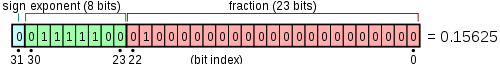
\includegraphics[scale=0.66]{structs/500px-Float_example.png}
\caption{\IFRU{Формат значения float (иллюстрация взята из wikipedia)}
{float value format (illustration taken from wikipedia)}}
\end{figure}

\lstinputlisting{structs/15_2_en.c}

\IFRU{Структура \TT{float\_as\_struct} занимает в памяти столько же места сколько и \Tfloat, 
то есть 4 байта или 32 бита.}
{\TT{float\_as\_struct} structure occupies as much space is memory as \Tfloat, e.g., 4 bytes or 32 bits.}

\IFRU{Далее мы выставляем во входящем значении отрицательный знак, 
а также прибавляя двойку к экспоненте, мы тем 
самым умножаем всё значение на \TT{$2^2$}, то есть на 4.}
{Now we setting negative sign in input value and also by addding 2 to exponent we thereby multiplicating
the whole number by \TT{$2^2$}, e.g., by 4.}

\IFRU{Компилируем в MSVC 2008 без оптимизации:}{Let's compile in MSVC 2008 without optimization:}

\IFRU{\lstinputlisting{structs/15_2_msvc_ru.asm}}{\lstinputlisting{structs/15_2_msvc_en.asm}}

\IFRU{Слекга избыточно. В версии скомпиленной с флагом \Ox нет вызовов \TT{memcpy()}, 
там работа происходит сразу с переменной f. Но по неоптимизированной версии будет проще понять.}
{Redundant for a bit. If it compiled with \Ox flag there are no \TT{memcpy()} call,
f variable is used directly. But it's easier to understand it all considering unoptimized version.}

\IFRU{А что сделает GCC 4.4.1 с опцией \TT{-O3}?}{What GCC 4.4.1 with \TT{-O3} will do?}

\lstinputlisting{structs/15_2_gcc_O3_en.asm}

\IFRU{Да, функция \TT{f()} в целом понятна. Однако, что интересно, еще при компиляции, 
не взирая на мешанину с полями структуры, GCC умудрился вычислить результат функции \TT{f(1.234)} и 
сразу подставить его в аргумент для \printf{}!}
{The \TT{f()} function is almost understandable. However, what is interesting, GCC was able to calculate
\TT{f(1.234)} result during compilation stage despite all this hodge-podge with structure fields
and prepared this argument to \printf{} as precalculated!}



% done

\section{\IFRU{Классы в Си++}{C++ classes}}

\IFRU{Я преднамеренно расположил описание классов здесь сразу за структурами, 
потому что внутреннее представление классов в Си++ почти такое же как и представление структур.}
{I placed a C++ classes description here intentionally after structures description,
because internally, C++ classes representation is almost the same as structures representation.}

\IFRU{Давайте попробуем простой пример с парой переменных, парой конструкторов и одним методом:}
{Let's try an example with two variables, couple of constructors and one method:}

\lstinputlisting{classes/16_1.cpp}

\IFRU{Вот как выглядит \main на ассемблере:}{Here is how \main function looks like translated into assembler:}

\lstinputlisting{classes/16_1_msvc.asm}

\IFRU{Вот что происходит. 
Под каждый экземпляр класса \IT{c} выделяется по 8 байт, столько же, сколько нужно 
для хранения двух переменных.}
{So what's going on.
For each object (instance of class \IT{c}) 8 bytes allocated, that's exactly size of 2 variables storage.}

\IFRU{Для \IT{c1} вызывается конструктор по умолчанию без аргументов \TT{??0c@@QAE@XZ}. 
Для \IT{c2} вызывается другой конструктор \TT{??0c@@QAE@HH@Z} и передаются два числа в качестве аргументов.}
{For \IT{c1} a default argumentless constructor \TT{??0c@@QAE@XZ} is called.
For \IT{c2} another constructor \TT{??0c@@QAE@HH@Z} is called and two numbers are passed as arguments.}

\IFRU{А указатель на объект (\IT{this} в терминологии Си++) передается в регистре \ECX. 
Это называется thiscall~\ref{thiscall} ~--- метод передачи указателя на объект.}
{A pointer to object (\IT{this} in C++ terminology) is passed in \ECX register.
This is called thiscall~\ref{thiscall} ~--- a pointer to object passing method.}

\IFRU{В данном случае, MSVC делает это через \ECX. Необходимо помнить, что это не стандартизированный метод, 
и другие компиляторы могут делать это иначе, например через первый аргумент функции (как GCC).}
{MSVC doing it using \ECX register. Needless to say, it's not a standardized method, other compilers could do it
differently, for example, via first function argument (like GCC).}

%\newcommand{\URLNM}{\href{http://en.wikipedia.org/wiki/Visual_C\%2B\%2B_name_mangling}{Wikipedia: Visual C++ name mangling}}
\newcommand{\URLNM}{\href{http://en.wikipedia.org/wiki/Name_mangling}{Wikipedia: Name mangling}}

\IFRU{Почему у имен функций такие странные имена? Это \IT{name mangling}\footnote{\URLNM}.}
{Why these functions has so odd names? That's \IT{name mangling}\footnote{\URLNM}.}

\IFRU{В Си++, у класса, может иметься несколько методов с одинаковыми именами 
но аргументами разных типов ~--- это полиморфизм. 
Ну и конечно, у разных классов могут быть методы с одинаковыми именами.}
{C++ class may contain several methods sharing the same name but having different arguments ~--- 
that's polymorphism.
And of course, different classes may own methods sharing the same name.}

\IFRU{\IT{Name mangling} позволяет закодировать имя класса + имя метода + типы всех аргументов метода 
в одной ASCII-строке, которая затем используется как внутреннее имя функции. 
Это все потому что ни линкер, ни загрузчик DLL операционной системы 
(мангленные имена могут быть среди экспортов/импортов в DLL), 
ничего не знают о Си++ или ООП.}
{\IT{Name mangling} allows to encode class name + method name + all method argument types 
in one ASCII-string, which will be used as internal function name.
That's all because neither linker, nor DLL operation system loader (mangled names may be among 
DLL exports as well) knows nothing about C++ or OOP.}

\IFRU{Далее вызывается два раза \TT{dump()}.}{\TT{dump()} function called two times after.}

\IFRU{Теперь смотрим на код в конструкторах:}{Now let's see constructors' code:}

\lstinputlisting{classes/16_2_msvc.asm}

\IFRU{Конструкторы это просто функции, они используют указатель на структуру в \ECX, 
перекладывают его себе в локальную переменную, хотя это и не обязательно.}
{Constructors are just functions, they use pointer to structure in \ECX,
moving the pointer into own local variable, however, it's not necessary.}

\IFRU{И еще метод \TT{dump()}:}{Now \TT{dump()} method:}

\lstinputlisting{classes/16_3_msvc.asm}

\IFRU{Все очень просто, \TT{dump()} берет указатель на структуру состоящую из двух \Tint через \ECX, 
выдергивает оттуда две переменные и передает их в \printf.}
{Simple enough: \TT{dump()} taking pointer to the structure containing two \Tint's in \ECX,
takes two values from it and passing it into \printf.}

\IFRU{А если скомпилировать с оптимизацией (\Ox), то будет намного меньше всего:}
{The code is much shorter if compiled with optimization (\Ox):}

\lstinputlisting{classes/16_4_msvc_Ox.asm}

\IFRU{Вот и все. Единственное о чем еще нужно сказать, это о том что в функции \main, 
когда вызывался второй конструктор с двумя аргументами, за ним не корректировался стек при помощи 
\TT{add esp, X}. В то же время, в конце у конструктора вместо \RET имеется \TT{RET 8}.}
{That's all. One more thing to say is that stack pointer after second constructor calling wasn't corrected
with \TT{add esp, X}. Please also note that, constructor has \TT{ret 8} instead of \RET at the end.}

\IFRU{Это потому что здесь используется thiscall~\ref{thiscall}, который, вместе с stdcall~\ref{stdcall} 
(все это ~--- методы передачи аргументов через стек), предлагает вызываемой функции корректировать стек. 
Инструкция \TT{ret X} сначала прибавляет \TT{X} к \ESP, затем передает управление вызывающей функции.}
{That's all because here used thiscall~\ref{thiscall} calling convention, the method of passing values through the
stack, which is, together with stdcall~\ref{stdcall} method, offers to correct stack to callee 
rather then to caller.
\TT{ret x} instruction adding \TT{X} to \ESP, then passes control to caller function.}

\IFRU{См.также в соответствующем разделе о способах передачи аргументов через стек}
{See also section about calling conventions}~\ref{sec:callingconventions}.

\IFRU{Еще, кстати, нужно отметить, что именно компилятор решает, когда вызывать конструктор и деструктор ~--- 
но это итак известно из основ языка Си++.}
{It's also should be noted that compiler deciding when to call constructor and destructor ~--- but that's 
we already know from C++ language basics.}

\subsection{GCC}

\IFRU{В GCC 4.4.1 все почти так же, за исключением некоторых различий.}
{It's almost the same situation in GCC 4.4.1, with few exceptions.}

\lstinputlisting{classes/16_5_gcc.asm}

\newcommand{\URLAGNER}{\url{http://www.agner.org/optimize/calling_conventions.pdf}}

\IFRU{Здесь мы видим что применяется иной \IT{name mangling} характерный для стандартов 
GNU\footnote{Еще о name mangling разных компиляторов: \URLAGNER}. Во-вторых, указатель на экземпляр передается как первый аргумент функции ~--- конечно же, скрыто от программиста.}
{Here we see another \IT{name mangling} style, specific to GNU\footnote{One more document about different compilers name mangling types: \URLAGNER} standards. It's also can be noted that pointer to object is passed as first function argument ~--- hiddenly from programmer, of course.}

\IFRU{Это первый конструктор:}{First constructor:}

\begin{lstlisting}
                public _ZN1cC1Ev ; weak
_ZN1cC1Ev       proc near               ; CODE XREF: main+10

arg_0           = dword ptr  8

                push    ebp
                mov     ebp, esp
                mov     eax, [ebp+arg_0]
                mov     dword ptr [eax], 667
                mov     eax, [ebp+arg_0]
                mov     dword ptr [eax+4], 999
                pop     ebp
                retn
_ZN1cC1Ev       endp
\end{lstlisting}

\IFRU{Он просто записывает два числа по указателю переданному в первом (и единственном) аргументе.}
{What it does is just writes two numbers using pointer passed in first (and sole) argument.}

\IFRU{Второй конструктор:}{Second constructor:}

\begin{lstlisting}
                public _ZN1cC1Eii
_ZN1cC1Eii      proc near

arg_0           = dword ptr  8
arg_4           = dword ptr  0Ch
arg_8           = dword ptr  10h

                push    ebp
                mov     ebp, esp
                mov     eax, [ebp+arg_0]
                mov     edx, [ebp+arg_4]
                mov     [eax], edx
                mov     eax, [ebp+arg_0]
                mov     edx, [ebp+arg_8]
                mov     [eax+4], edx
                pop     ebp
                retn
_ZN1cC1Eii      endp
\end{lstlisting}

\IFRU{Эта функция, аналог которой мог бы выглядеть так:}{This is a function, analog of which could be looks like:}

\begin{lstlisting}
void ZN1cC1Eii (int *obj, int a, int b)
{
  *obj=a;
  *(obj+1)=b;
};
\end{lstlisting}

\IFRU{... что, в общем, предсказуемо.}{... and that's completely predictable.}

\IFRU{И функция \TT{dump()}:}{Now \TT{dump()} function:}

\begin{lstlisting}
                public _ZN1c4dumpEv
_ZN1c4dumpEv    proc near

var_18          = dword ptr -18h
var_14          = dword ptr -14h
var_10          = dword ptr -10h
arg_0           = dword ptr  8

                push    ebp
                mov     ebp, esp
                sub     esp, 18h
                mov     eax, [ebp+arg_0]
                mov     edx, [eax+4]
                mov     eax, [ebp+arg_0]
                mov     eax, [eax]
                mov     [esp+18h+var_10], edx
                mov     [esp+18h+var_14], eax
                mov     [esp+18h+var_18], offset aDD ; "%d; %d\n"
                call    _printf
                leave
                retn
_ZN1c4dumpEv    endp
\end{lstlisting}

\IFRU{Эта функция \IT{во внутреннем представлении} имеет один аргумент, через который передается указатель на 
объект\footnote{экземпляр класса} (\IT{this}).}
{This function in its \IT{internal representation} has sole argument, 
used as pointer to the object (\IT{this}).}

\IFRU{Таким образом, если брать в учет только эти простые примеры, разница между MSVC и GCC 
в способе кодирования имен функций (\IT{name mangling}) и передаче указателя на экземпляр класса 
(через \ECX или через первый аргумент).}
{Thus, if to base our judgment on these simple examples, the difference between MSVC and GCC
is style of function names encoding (\IT{name mangling}) and passing pointer to object
(via \ECX register or via first argument).}

% TODO: RTTI

\section{unions}

% done

\subsection{\IFRU{Пример генератора случайных чисел}{Pseudo-random number generator example}}

\IFRU{Если нам нужны случайные значения с плавающей запятой в интервале от 0 до 1, самое простое это взять
генератор ПСЧ вроде Mersenne twister выдающий случайные 32-битные числа в виде DWORD, преобразовать
это число в \Tfloat и затем разделить на \TT{RAND\_MAX} (\IT{0xffffffff} в данном случае) ~--- 
полученное число будет в интервале от 0 до 1.}
{If we need float random numbers from 0 to 1, the most simplest thing is to use random numbers generator like
Mersenne twister producing random 32-bit values in DWORD form, transform this value to \Tfloat and then
divide it by \TT{RAND\_MAX} (\IT{0xffffffff} in our case) ~--- value we got will be in 0..1 interval.}

\IFRU{Но как известно, операция деления это медленная операция почти всегда. 
Сможем ли мы избежать её, как в случае с делением через умножение?}
{But as we know, division operation is almost always very slow.
Will it be possible to get rid of it, as in case of division by multiplication?}
~\ref{sec:divisionbynine}

\IFRU{Вспомним состав числа с плавающей запятой: это бит знака, биты мантиссы и биты экпоненты. 
Для получения случайного числа, нам нужно просто заполнить случайными битами все биты мантиссы!}
{Let's remember what float number consisted of: sign bit, significand bits and exponent bits.
We need just to store random bits to significand bits for getting float number!}

\IFRU{Экспонента не может быть нулевой (иначе число будет денормализованным), 
так что в эти биты мы запишем \IT{01111111} ~--- 
это будет означать что экспонента равна единице. Далее заполняем мантиссу случайными битами, 
знак оставляем в виде 0 (что значит наше число положительное), и вуаля. 
Генерируемые числа будут в интервале от 1 до 2, так что нам еще нужно будет отнять единицу.}
{Exponent cannot be zero (number will be denormalized in this case), so we will store \IT{01111111} 
to exponent ~--- this mean exponent will be 1. Then fill significand with random bits, set sign bit to
0 (which mean positive number) and voilà.
Generated numbers will be in 1 to 2 interval, so we also should subtract 1 from it.}

\newcommand{\URLXOR}{\url{http://xor0110.wordpress.com/2010/09/24/how-to-generate-floating-point-random-numbers-efficiently}}

\IFRU{В моем примере\footnote{идея взята здесь: \URLXOR} 
применяется очень простой линейный конгруэнтный генератор случайных чисел, выдающий 32-битные числа.
Генератор инициализируется текущим временем в стиле UNIX.}
{Very simple linear congruential random numbers generator is used in my 
example\footnote{idea was taken from: \URLXOR}, producing 32-bit numbers. 
The PRNG initializing by current time in UNIX-style.}

\IFRU{Далее, тип \Tfloat представляется в виде \IT{union} ~--- это конструкция \CCpp позволяющая 
интерпретировать часть памти по-разному. В нашем случае, мы можем создать переменную типа \TT{union} 
и затем обращаться к ней как к \Tfloat или как к \IT{uint32\_t}. Можно сказать что это хак, причем грязный.}
{Then, \Tfloat type represented as \IT{union} ~--- that is the \CCpp construction allowing us
to interpret piece of memory differently typed. In our case, we are able to create a variable
of \TT{union} type and then access to it as it's \Tfloat or as it's \IT{uint32\_t}. 
It can be said, it's just a hack. A dirty one.}

\lstinputlisting{unions/FPU_PRNG.cpp}

MSVC 2010 (\Ox): 

\lstinputlisting{\IFRU{unions/FPU_PRNG_msvc_2010_Ox_ru.asm}{unions/FPU_PRNG_msvc_2010_Ox_en.asm}}

\IFRU{А результат GCC будет почти таким же.}{GCC producing very same code.}





% done

\section{\IFRU{Указатели на функции}{Pointers to functions}}
\label{sec:pointerstofunctions}

\IFRU{Указатель на функцию, в целом, как и любой другой указатель, просто адрес указывающий на начало функции 
в сегменте кода.}
{Pointer to function, as any other pointer, is just an address of function beginning in its code segment.}

\IFRU{Это применяется часто в т.н. callback-ах}{It is often used in callbacks}
\footnote{\url{http://en.wikipedia.org/wiki/Callback_(computer_science)}}.

\IFRU{Известные примеры:}{Well-known examples are:}

\begin{itemize}
\item
\qsort\footnote{\url{http://en.wikipedia.org/wiki/Qsort_(C_standard_library)}},
{\TT{atexit()}}\footnote{\url{http://www.opengroup.org/onlinepubs/009695399/functions/atexit.html}} \IFRU{из стандартной библиотеки Си}{from the standard C library}; 
\item
\IFRU{сигналы в *NIX ОС}{signals in *NIX OS}\footnote{\url{http://en.wikipedia.org/wiki/Signal.h}};
\item
\IFRU{запуск тредов}{thread starting}: \TT{CreateThread()} (win32), \TT{pthread\_create()} (POSIX);
\item
\IFRU{множество функций win32, например}{a lot of win32 functions, for example} \TT{EnumChildWindows()}\footnote{\url{http://msdn.microsoft.com/en-us/library/ms633494(VS.85).aspx}}.
\end{itemize}

\IFRU{Итак, функция \qsort это реализация алгоритма "быстрой сортировки". 
Функция может сортировать что угодно, 
любые типы данных, но при условии что вы имеете функцию сравнения двух элементов данных и 
\qsort может вызывать её.}
{So, \qsort function is a \CCpp standard library quicksort implemenation. The functions is able to sort
anything, any types of data, if you have a function for two elements comparison and \qsort is able
to call it.}

\IFRU{Эта функция сравнения может определяться так:}{The comparison function can be defined as:}

\begin{lstlisting}
int (*compare)(const void *, const void *)
\end{lstlisting}

\IFRU{Воспользуемся немного модифицированным примером, который я нашел вот}
{Let's use slightly modified example I found} \href{http://cplus.about.com/od/learningc/ss/pointers2_8.htm}
{\IFRU{здесь}{here}}:

\lstinputlisting{pointers_to_functions/17_1.c}

\IFRU{Компилируем в MSVC 2010 (я убрал некоторые части для краткости) с опцией \Ox}
{Let's compile it in MSVC 2010 (I omitted some parts for the sake of brefity) with \Ox option}:

\lstinputlisting{pointers_to_functions/17_2_msvc_Ox.asm}

\IFRU{Ничего особо удивительного здесь мы не видим. В качестве четвертого аргумента, 
в \qsort просто передается адрес метки \TT{\_comp}, где собственно и располагается функция \TT{comp()}.}
{Nothing surprising so far. As a fourth argument, an address of label \TT{\_comp} is passed, that's just a place
where function \TT{comp()} located.}

\IFRU{Как \qsort вызывает её?}{How \qsort calling it?}

\IFRU{Посмотрим в MSVCR80.DLL (эта DLL куда в MSVC вынесены функции из стандартных библиотек Си):}
{Let's take a look into this function located in MSVCR80.DLL (a MSVC DLL module with C standard library functions):}

\lstinputlisting{pointers_to_functions/17_3_MSVCR.lst}

\IFRU{\TT{comp} ~--- это четвертый аргумент функции. 
Здесь просто передается управление по адресу указанному в \TT{comp}. 
Перед этим подготавливается два аргумента для функции \TT{comp()}. Далее, проверяется результат её выполнения.}
{\TT{comp} ~--- is fourth function argument.
Here the control is just passed to the address in \TT{comp}.
Before it, two arguments prepared for \TT{comp()}. Its result is checked after its execution.}

\IFRU{Вот почему использование указателей на функции ~--- это опасно. 
Во-первых, если вызвать \qsort с неправильным указателем на функцию, 
то \qsort, дойдя до этого вызова, может передать управление неизвестно куда, 
процесс упадет, и эту ошибку можно будет найти не сразу.}
{That's why it's dangerous to use pointers to functions.
First of all, if you call \qsort with incorrect pointer to function, \qsort may pass control
to incorrect place, process may crash and this bug will be hard to find.}

\IFRU{Во-вторых, типизация callback-функции должна строго соблюдаться, 
вызов не той функции с не теми аргументами не того типа, 
может привести к плачевным результатам, 
хотя падение процесса это и не проблема ~--- а проблема это найти ошибку ~--- ведь компилятор 
на стадии компиляции может вас и не предупредить о потенциальных неприятностях.}
{Second reason is that callback function types should comply strictly, calling wrong function
with wrong arguments of wrong types may lead to serious problems, however, process crashing is not a 
big problem ~--- big problem is to determine a reason of crashing ~--- because compiler may be 
silent about potential trouble while compiling.}

\subsection{GCC}

\IFRU{Не слишком большая разница:}{Not a big difference:}

\begin{lstlisting}
                lea     eax, [esp+40h+var_28]
                mov     [esp+40h+var_40], eax
                mov     [esp+40h+var_28], 764h
                mov     [esp+40h+var_24], 2Dh
                mov     [esp+40h+var_20], 0C8h
                mov     [esp+40h+var_1C], 0FFFFFF9Eh
                mov     [esp+40h+var_18], 0FF7h
                mov     [esp+40h+var_14], 5
                mov     [esp+40h+var_10], 0FFFFCFC7h
                mov     [esp+40h+var_C], 43Fh
                mov     [esp+40h+var_8], 58h
                mov     [esp+40h+var_4], 0FFFE7960h
                mov     [esp+40h+var_34], offset comp
                mov     [esp+40h+var_38], 4
                mov     [esp+40h+var_3C], 0Ah
                call    _qsort
\end{lstlisting}

\IFRU{Функция \TT{comp()}}{\TT{comp()} function}:

\begin{lstlisting}
                public comp
comp            proc near

arg_0           = dword ptr  8
arg_4           = dword ptr  0Ch

                push    ebp
                mov     ebp, esp
                mov     eax, [ebp+arg_4]
                mov     ecx, [ebp+arg_0]
                mov     edx, [eax]
                xor     eax, eax
                cmp     [ecx], edx
                jnz     short loc_8048458
                pop     ebp
                retn
loc_8048458:
                setnl   al
                movzx   eax, al
                lea     eax, [eax+eax-1]
                pop     ebp
                retn
comp            endp
\end{lstlisting}

\IFRU{Реализация \qsort находится в \TT{libc.so.6}, и представляет собой просто враппер для \TT{qsort\_r()}.}
{\qsort implementation is located in \TT{libc.so.6} and it is in fact just a wrapper for \TT{qsort\_r()}.}

\IFRU{Она, в свою очередь, вызывает \TT{quicksort()}, где есть вызовы определенной нами функции через 
переданный указатель:}
{It will call then \TT{quicksort()}, where our defined function will be called via passed pointer:}

\IFRU{(файл libc.so.6, версия glibc ~--- 2.10.1)}{(File libc.so.6, glibc version ~--- 2.10.1)}

\begin{lstlisting}
.text:0002DDF6                 mov     edx, [ebp+arg_10]
.text:0002DDF9                 mov     [esp+4], esi
.text:0002DDFD                 mov     [esp], edi
.text:0002DE00                 mov     [esp+8], edx
.text:0002DE04                 call    [ebp+arg_C]
...
\end{lstlisting}


% done

\section{SIMD}

SIMD \IFRU{это акроним:}{is just acronym:} \IT{Single Instruction, Multiple Data}.

\IFRU{Как можно судить по названию, это обработка множества данных исполняя только одну инструкцию.}
{As it's said, it's multiple data processing using only one instruction.}

\IFRU{Как и FPU, эта подсистема процессора выглядит также отдельным процессором внутри x86.}
{Just as FPU, that CPU subsystem looks like separate processor inside x86.}

\IFRU{SIMD в x86 начался с MMX. Появилось 8 64-битных регистров MM0-MM7.}
{SIMD began as MMX in x86. 8 new 64-bit registers appeared: MM0-MM7.}

\IFRU{Каждый MMX-регистр может содержать 2 32-битных значения, 4 16-битных или же 8 байт. 
Например, складывая значения двух MMX-регистров, можно складывать одновременно 8 8-битных значений.}
{Each MMX register may hold 2 32-bit values, 4 16-bit values or 8 bytes.
For example, it is possible to add 8 8-bit values (bytes) simultaneously by adding two values in MMX-registers.}

\IFRU{Простой пример, это некий графический редактор, который хранит открытое изображение как двумерный массив. 
Когда пользователь меняет яркость изображения, редактору нужно, например, прибавить некий коэффициент 
ко всем пикселям, или отнять. 
Для простоты можно представить, что изображение у нас бело-серо-черное и каждый пиксель занимает один байт, 
то с помощью MMX можно менять яркость сразу у восьми пикселей.}
{One simple example is graphics editor, representing image as a two dimensional array.
When user change image brightness, the editor should add some coefficient to each pixel value, or to subtract.
For the sake of brevity, our image may be grayscale and each pixel defined by one 8-bit byte, then it's possible
to change brightness of 8 pixels simultaneously.}

\IFRU{Когда MMX только появилось, эти регистры на самом деле распологались в FPU-регистрах. 
Можно было использовать 
либо FPU либо MMX в одно и то же время. Можно подумать что Intel решило немного сэкономить на транзисторах, 
но на самом деле причина такого симбиоза проще ~--- более старая операционная система не знающая о дополнительных 
регистрах процессора не будет сохранять их во время переключения задач, а вот регистры FPU сохранять будет. 
Таким образом, процессор с MMX + старая операционная система + задача использующая MMX = все 
это может работать вместе.}
{When MMX appeared, these registers was actually located in FPU registers. 
It was possible to use either FPU or MMX at the same time. One might think, Intel saved on transistors,
but in fact, the reason of such symbiosis is simpler ~--- older operation system may not aware 
of additional CPU registers wouldn't save them at the context switching, but will save FPU registers.
Thus, MMX-enabled CPU + old operation system + process using MMX = that all will work together.}

SSE ~--- \IFRU{это расширение регистров до 128 бит, теперь уже отдельно от FPU.}{is extension of SIMD registers up to 128 bits, now separately from FPU.}

AVX ~--- \IFRU{расширение регистров до 256 бит.}{another extension to 256 bits.}

\IFRU{Немного о практическом применении.}{Now about practical usage.}

\IFRU{Конечно же, копирование блоков в памяти (\TT{memcpy}), сравнение (\TT{memcmp}), и подобное.}
{Of course, memory copying (\TT{memcpy}), memory comparing (\TT{memcmp}) and so on.}

\IFRU{Еще пример: имеется алгоритм шифрования DES, который берет 64-битный блок, 56-битный ключ, 
шифрует блок с ключем и образуется 64-битный результат.
Алгоритм DES можно легко представить в виде очень большой электронной цифровой схемы, 
с проводами, элементами И, ИЛИ, НЕ.}
{One more example: we got DES encryption algorithm, it takes 64-bit block, 56-bit key, encrypt block and produce 64-bit result.
DES algorithm may be considered as a very large electronic circuit, with wires and AND/OR/NOT gates.}

\label{bitslicedes}
\newcommand{\URLBS}{\url{http://www.darkside.com.au/bitslice/}}

\IFRU{Идея bitslice DES\footnote{\URLBS} ~--- это обработка сразу группы блоков и ключей одновременно. 
Скажем, на x86 перменная типа \IT{unsigned int} вмещает в себе 32 бита, так что там можно хранить 
промежуточные результаты сразу для 32-х блоков-ключей, используя 64+56 переменных типа \IT{unsigned int}.}
{Bitslice DES\footnote{\URLBS} ~--- is an idea of processing group of blocks and keys simultaneously.
Let's say, variable of type \IT{unsigned int} on x86 may hold up to 32 bits, so, it's possible to store there
intermediate results for 32 blocks-keys pairs simultaneously, using 64+56 variables of \IT{unsigned int} type.}

\IFRU{Я написал утилиту для перебора паролей/хешей Oracle RDBMS (которые основаны на алгоритме DES), 
переделав алгоритм bitslice DES для SSE2 и AVX ~--- и теперь возможно шифровать одновременно 
128 или 256 блоков-ключей:}
{I wrote an utility to brute-force Oracle RDBMS passwords/hashes (ones based on DES),
slightly modified bitslice DES algorithm for SSE2 and AVX ~--- now it's possible to encrypt 128 
or 256 block-keys pairs simultaneously.}

\url{http://conus.info/utils/ops_SIMD/}
 
\subsection{\IFRU{Векторизация}{Vectorization}}

\newcommand{\URLVEC}{\href{http://en.wikipedia.org/wiki/Vectorization_(computer_science)}{Wikipedia: vectorization}}

\IFRU{Векторизация\footnote{\URLVEC} это когда у вас есть цикл, который берет на вход несколько массивов и выдает, 
например, один массив данных. 
Тело цикла берет некоторые элементы из входных массивов, что-то делает с ними и кладет в выходной. 
Важно что операция применяемая ко всем элементам одна и та же. 
Векторизация ~--- это обрабатывать несколько элементов одновременно.}
{Vectorization\footnote{\URLVEC}, for example, is when you have a loop taking couple of arrays at input and producing one array.
Loop body takes values from input arrays, do something and put result into output array.
It's important that there is only one single operation applied to each element.
Vectorization ~--- is to process several elements simultaneously.}

\IFRU{Например:}{For example:}

\begin{lstlisting}
for (i = 0; i < 1024; i++)
{
    C[i] = A[i]*B[i];
}
\end{lstlisting}

\IFRU{Этот кусок кода берет элементы из A и B, перемножает и сохраняет результат в C.}
{This piece of code takes elements from A and B, multiplies them and save result into C.}

\newcommand{\PMULLD}{\IT{PMULLD} (\IT{\IFRU{Перемножить запакованные знаковые DWORD и сохранить младшую часть результата}
{Multiply Packed Signed Dword Integers and Store Low Result}})}
\newcommand{\PMULHW}{\TT{PMULHW} (\IT{\IFRU{Перемножить апакованные знаковые DWORD и сохранить старшую часть результата}
{Multiply Packed Signed Integers and Store High Result}})}

\IFRU{Если представить что каждый элемент массива ~--- это 32-битный \Tint, то их можно загружать сразу 
по 4 из А в 128-битный XMM-регистр, 
из B в другой XMM-регистр и выполнив инстукцию \PMULLD и \PMULHW, можно получить 4 64-битных 
произведения\footnote{результат умножения} сразу.}
{If each array element we have is 32-bit \Tint, then it's possible to load 4 elements from A into 128-bit 
XMM-register, from B to another XMM-registers, and by executing \PMULLD and \PMULHW, 
it's possible to get 4 64-bit products\footnote{multiplication result} at once.}

\IFRU{Таким образом, тело цикла исполняется 1024/4 раза вместо 1024, что в 4 раза меньше, и, конечно, быстрее.}
{Thus, loop body count is 1024/4 instead of 1024, that's 4 times less and, of course, faster.}

\newcommand{\URLINTELVEC}{\href{http://www.intel.com/intelpress/sum_vmmx.htm}{Excerpt: Effective Automatic Vectorization}}

\IFRU{Некоторые компиляторы умеют делать автоматическую векторизацию в простых случаях, 
например Intel C++\footnote{Еще о том как Intel C++ умеет автоматически векторизировать циклы: \URLINTELVEC}.}
{Some compilers can do vectorization automatically in some simple cases, 
for example, Intel C++\footnote{More about Intel C++ automatic vectorization: \URLINTELVEC}.}

\IFRU{Я написал очень простую функцию:}{I wrote tiny function:}

\begin{lstlisting}
int f (int sz, int *ar1, int *ar2, int *ar3)
{
	for (int i=0; i<sz; i++)
		ar3[i]=ar1[i]+ar2[i];

	return 0;
};
\end{lstlisting}

\subsubsection{Intel C++}

\IFRU{Компилирую при помощи}{Let's compile it with} Intel C++ 11.1.051 win32:

\begin{verbatim}
icl intel.cpp /QaxSSE2 /Faintel.asm /Ox
\end{verbatim}

\IFRU{Имеем такое (в \IDA):}{We got (in \IDA):}

\lstinputlisting{SIMD/18_1_en.asm}

\IFRU{Инструкции имеющие отношение к SSE2 это:}{SSE2-related instructions are:}

\begin{itemize}
\item
\MOVDQU (\IT{Move Unaligned Double Quadword}) ~--- \IFRU{она просто загружает 16 байт из памяти в XMM-регистр}
{it just load 16 bytes from memory into XMM-register}.

\item
\PADDD (\IT{Add Packed Integers}) ~--- 
\IFRU{складывает сразу 4 пары 32-битных чисел чисел и оставляет в первом операнде результат. 
Кстати, если произойдет переполнение, то исключения не произойдет и никакие флаги не установятся, 
запишутся просто младшие 32 бита результата. 
Если один из операндов \PADDD ~--- адрес значения в памяти, 
то требуется чтобы адрес был выровнен по 16-байтной границе. Если он не выровнен, произойдет исключение
\footnote{О выравнивании данных см. также: \URLWPDA}.}
{adding 4 pairs of 32-bit numbers and leaving result in first operand.
By the way, no exception raised in case of overflow and no flags will be set, just low 32-bit of result will
be stored.
If one of \PADDD operands ~--- address of value in memory,
address should be aligned by 16-byte border. If it's not aligned, exception will be raised
\footnote{More about data aligning: \URLWPDA}.}

\item
\MOVDQA (\IT{Move Aligned Double Quadword}) ~--- \IFRU{тоже что и \MOVDQU, только подразумевает 
что адрес в памяти выровнен по 16-байтной границе. 
Если он не выровнен, произойдет исключение. 
\MOVDQA работает быстрее чем \MOVDQU, но требует вышеозначенного.}
{the same as \MOVDQU, but requires address of value in memory to be aligned by 16-bit border.
If it's not aligned, exception will be raised.
\MOVDQA works faster than \MOVDQU, but requires aforesaid.}

\end{itemize}

\IFRU{Итак, эти SSE2-инструкции исполнятся только в том случае если еще осталось просуммировать 
4 пары переменных типа \Tint плюс если указатель \TT{ar3} выровнен по 16-байтной границе.}
{So, these SSE2-instructions will be executed only in case if there are more 4 pairs to work on
plus pointer \TT{ar3} is aligned on 16-byte border.}

\IFRU{Более того, если еще и \TT{ar2} выровнен по 16-байтной границе, то будет выполняться этот кусок:}
{More than that, if \TT{ar2} is aligned on 16-byte border too, this piece of code will be executed:}

\begin{lstlisting}
movdqu  xmm0, xmmword ptr [ebx+edi*4] ; ar1+i*4
paddd   xmm0, xmmword ptr [esi+edi*4] ; ar2+i*4
movdqa  xmmword ptr [eax+edi*4], xmm0 ; ar3+i*4
\end{lstlisting}

\IFRU{А иначе, значение из \TT{ar2} загрузится в \XMMZERO используя инструкцию \MOVDQU, 
которая не требует выровненного указателя, зато может работать чуть медленнее:}
{Otherwise, value from \TT{ar2} will be loaded to \XMMZERO using \MOVDQU,
it doesn't require aligned pointer, but may work slower:}

\begin{lstlisting}
movdqu  xmm1, xmmword ptr [ebx+edi*4] ; ar1+i*4
movdqu  xmm0, xmmword ptr [esi+edi*4] ; ar2+i*4 is not 16-byte aligned, so load it to xmm0
paddd   xmm1, xmm0
movdqa  xmmword ptr [eax+edi*4], xmm1 ; ar3+i*4
\end{lstlisting}

\IFRU{А во всех остальных случаях, будет исполняться код, который был бы как если бы не была 
включена поддержка SSE2.}
{In all other cases, non-SSE2 code will be executed.}

\subsubsection{GCC}

\newcommand{\URLGCCVEC}{\url{http://gcc.gnu.org/projects/tree-ssa/vectorization.html}}

\IFRU{Но и GCC умеет кое-что векторизировать\footnote{Подробнее о векторизации в GCC: \URLGCCVEC}, 
если компилировать с опциями \TT{-O3} и включить поддержку SSE2: \TT{-msse2}.}
{GCC may also vectorize in some simple cases\footnote{More about GCC vectorization support: \URLGCCVEC},
if to use \TT{-O3} option and to turn on SSE2 support: \TT{-msse2}.}

\IFRU{Вот что вышло}{What we got} (GCC 4.4.1):

\lstinputlisting{SIMD/18_2_gcc_O3.asm}

\IFRU{Почти то же самое, хотя и не так дотошно как Intel C++.}
{Almost the same, however, not as meticulously as Intel C++ doing it.}

\subsection{\IFRU{Реализация \strlen при помощи SIMD}{SIMD \strlen implementation}}

\newcommand{\URLMSDNSSE}{\href{http://msdn.microsoft.com/en-us/library/y0dh78ez(VS.80).aspx}{MSDN: MMX, SSE, and SSE2 Intrinsics}}

\IFRU{Прежде всего, следует заметить, что SIMD-инструкции можно вставлять в \CCpp код при помощи специальных 
макросов\footnote{\URLMSDNSSE}. В MSVC, часть находится в файле \TT{intrin.h}.}
{It should be noted that SIMD-instructions may be inserted into \CCpp code via 
special macros\footnote{\URLMSDNSSE}.
As of MSVC, some of them are located in \TT{intrin.h} file.}

\IFRU{Имеется возможность реализовать функцию \strlen\footnote{strlen() ~--- стандартная функция Си 
для подсчета длины строки} при помощи SIMD-инструкций, работающий в 2-2.5 раза быстрее обычной реализации. 
Эта функция будет загружать в XMM-регистр сразу 16 байт и проверять каждый на ноль.}
{It is possible to implement \strlen function\footnote{strlen() ~--- standard C library function for calculating
string length} using SIMD-instructions, working 2-2.5 times faster than usual implementation.
This function will load 16 characters into XMM-register and check each against zero.}

\lstinputlisting{SIMD/18_3.c}

\newcommand{\URLSTRLEN}{http://www.strchr.com/sse2\_optimised\_strlen}

\IFRU{(пример базируется на исходнике \href{\URLSTRLEN}{отсюда}).}
{(the example is based on source code from \href{\URLSTRLEN}{there}).}

\IFRU{Компилируем в MSVC 2010 с опцией \Ox:}{Let's compile in MSVC 2010 with \Ox option:}

\lstinputlisting{SIMD/18_4_msvc_Ox.asm}

\IFRU{Итак, прежде всего, мы проверяем указатель \TT{str}, выровнен ли он по 16-байтной границе. 
Если нет, то мы вызовем обычную реализацию \strlen.}
{First of all, we check \TT{str} pointer, if it's aligned by 16-byte border.
If not, let's call usual \strlen implementation.}

\IFRU{Далее мы загружаем по 16 байт в регистр \XMMONE при помощи команды \MOVDQA.}
{Then, load next 16 bytes into \XMMONE register using \MOVDQA instruction.}

\IFRU{Наблюдательный читатель может спросить, почему в этом месте мы не можем использовать \MOVDQU, 
которая может загружать откуда угодно не взирая на факт, выровнен ли указатель?}
{Observant reader might ask, why \MOVDQU cannot be used here, because it can load data from the memory
regardless the fact if the pointer aligned or not.}

\IFRU{Да, можно было бы сделать вот как: если указатель выровнен, загружаем используя \MOVDQA, 
иначе используем работающую чуть медленнее \MOVDQU.}
{Yes, it might be done in this way: if pointer is aligned, load data using \MOVDQA,
if not ~--- use slower \MOVDQU.}

\IFRU{Однако здесь кроется не сразу заметная проблема, которая проявляется вот в чем:}
{But here we are may stick into hard to notice problem:}

\newcommand{\URLPAGE}{\url{http://en.wikipedia.org/wiki/Page_(computer_memory)}}

\IFRU{В ОС линии Windows NT\footnote{Windows NT, 2000, XP, Vista, 7, 8}, и не только, память выделяется страницами по 4 KiB (4096 байт). 
Каждый win32-процесс якобы имеет в наличии 4 GiB, но на самом деле, 
только некоторые части этого адресного пространства присоеденены к реальной физической памяти. 
Если процесс обратится к блоку памяти, которого не существует, сработает исключение. 
Так работает виртуальная память\footnote{\URLPAGE}.}
{In Windows NT line of operation systems\footnote{Windows NT, 2000, XP, Vista, 7, 8}, but not limited to it, memory allocated by pages of 4 KiB (4096 bytes).
Each win32-process has ostensibly 4 GiB, but in fact, only some parts
of address space are connected to real physical memory.
If the process accessing to the absent memory block, exception will be raised.
That's how virtual memory works\footnote{\URLPAGE}.}

\IFRU{Так вот, функция, читающая сразу по 16 байт, имеет возможность нечаянно вылезти за границу 
выделенного блока памяти. 
Предположим, ОС выделила программе 8192 (0x2000) байт по адресу 0x008c0000. 
Таким образом, блок занимает байты с адреса 0x008c0000 по 0x008c1fff включительно.}
{So, some function loading 16 bytes at once, may step over a border of allocated memory block.
Let's consider, OS allocated 8192 (0x2000) bytes at the address 0x008c0000.
Thus, the block is the bytes starting from address 0x008c0000 to 0x008c1fff inclusive.}

\IFRU{За этим блоком, то есть начиная с адреса 0x008c2000 нет вообще ничего, т.е., ОС не выделяла там память. 
Обращение к памяти начиная с этого адреса вызовет исключение.}
{After that block, that is, starting from address 0x008c2008 there are nothing at all, e.g., OS not allocated
any memory there. Attempt to access a memory starting from that address will raise exception.}

\IFRU{И предположим, что программа хранит некую строку из, скажем, пяти символов почти в самом конце блока, 
что не является преступлением:}
{And let's consider, the program holding some string containing 5 characters almost at the end of block,
and that's not a crime.}

\begin{center}
  \begin{tabular}{ | l | l | }
    \hline
        0x008c1ff8 & 'h' \\
        0x008c1ff9 & 'e' \\
        0x008c1ffa & 'l' \\
        0x008c1ffb & 'l' \\
        0x008c1ffc & 'o' \\
        0x008c1ffd & '\textbackslash{}x00' \\
        0x008c1ffe & \IFRU{здесь случайный мусор}{random noise} \\
        0x008c1fff & \IFRU{здесь случайный мусор}{random noise} \\
    \hline
  \end{tabular}
\end{center}

\IFRU{В обычных условиях, программа вызвает \strlen передав ей указатель на строку \TT{'hello'} 
лежащую по адресу 0x008c1ff8. 
\strlen будет читать по одному байту до 0x008c1ffd, где ноль, и здесь она закончит работу.}
{So, in usual conditions the program calling \strlen passing it a pointer to string \TT{'hello'} 
lying in memory at address 0x008c1ff8.
\strlen will read one byte at a time until 0x008c1ffd, where zero-byte, and so here it will stop working.}

\IFRU{Теперь, если мы напишем свою реализацию \strlen читающую сразу по 16 байт, с любого адреса, 
будь он выровнен по 16-байтной границе или нет, 
\MOVDQU попытается загрузить 16 байт с адреса 0x008c1ff8 по 0x008c2008, и произойдет исключение. 
Это ситуация которой, конечно, хочется избежать.}
{Now if we implement own \strlen reading 16 byte at once, starting at any address, will it be alligned or not,
\MOVDQU may attempt to load 16 bytes at once at address 0x008c1ff8 up to 0x008c2008, 
and then exception will be raised.
That's the situation to be avoided, of course.}

\IFRU{Поэтому мы будем работать только с адресами выровненными по 16 байт, что в сочетании со знанием 
что размер страницы также как правило выровнен по 16 байт, 
даст некоторую гарантию что наша функция не будет пытаться читать из мест в невыделенной памяти.}
{So then we'll work only with the addresses aligned by 16 byte border, what in combination with a knowledge
of operation system page size is usually aligned by 16 byte too, give us some warranty our function will not
read from unallocated memory.}

\IFRU{Вернемся к нашей функции}{Let's back to our function}.

\verb|_mm_setzero_si128()| ~--- \IFRU{это макрос, генерирующий \TT{pxor xmm0, xmm0} ~--- инструкция просто обнуляет регистр \XMMZERO.}
{is a macro generating \TT{pxor xmm0, xmm0} ~--- instruction just clear /XMMZERO register}

\verb|_mm_load_si128()| ~--- \IFRU{это макрос для \MOVDQA, он просто загружает 16 байт по адресу из указателя в \XMMONE.}
{is a macro for \MOVDQA, it just loading 16 bytes from the address in \XMMONE.}

\verb|_mm_cmpeq_epi8()| ~--- \IFRU{это макрос для \PCMPEQB, это инструкция которая 
побайтово сравнивает значения из двух XMM регистров.} 
{is a macro for \PCMPEQB, is an instruction comparing two XMM-registers bytewise.}

\IFRU{И если какой-то из байт равен другому, то в результирующем значении будет выставлено на месте этого 
байта 0xff, либо 0, если байты не были равны.}
{And if some byte was equals to other, there will be 0xff at this place in result or 0 if otherwise.}

\IFRU{Например.}{For example.}

\begin{verbatim}
XMM1: 11223344556677880000000000000000
XMM0: 11ab3444007877881111111111111111
\end{verbatim}

\IFRU{После исполнения \TT{pcmpeqb xmm1, xmm0}, регистр \XMMONE будет содержать:}
{After \TT{pcmpeqb xmm1, xmm0} execution, \XMMONE register will contain:}

\begin{verbatim}
XMM1: ff0000ff0000ffff0000000000000000
\end{verbatim}

\IFRU{Эта инструкция в нашем случае, сравнивает каждый 16-байтный блок с блоком состоящим из 16-и нулевых байт, 
выставленным в \XMMZERO при помощи \TT{pxor xmm0, xmm0}.}
{In our case, this instruction comparing each 16-byte block with the block of 16 zero-bytes,
was set in \XMMZERO by \TT{pxor xmm0, xmm0}.}

\IFRU{Следующий макрос \TT{\_mm\_movemask\_epi8()} ~--- это инструкция \TT{PMOVMSKB}.}
{The next macro is \TT{\_mm\_movemask\_epi8()} ~--- that is \TT{PMOVMSKB} instruction.}

\IFRU{Она очень удобна как раз для использования в паре с \PCMPEQB.}
{It is very useful if to use it with \PCMPEQB.}

\TT{pmovmskb eax, xmm1}

\IFRU{Эта инструкция выставит самый первый бит \EAX в единицу, если старший бит первого байта в 
регистре \XMMONE является единицей. 
Иными словами, если первый байт в регистре \XMMONE является 0xff, то первый бит в \EAX будет также единицей, 
иначе нулем.}
{This instruction will set first \EAX bit into 1 if most significant bit of the first byte in \XMMONE is 1.
In other words, if first byte of \XMMONE register is 0xff, first \EAX bit will be set to 1 too.}

\IFRU{Если второй байт в регистре \XMMONE является 0xff, то второй бит в \EAX также будет единицей. 
Иными словами, инструкция отвечает на вопрос, \IT{какие из байт в \XMMONE являются 0xff?}
В результате приготовит 16 бит и запишет в \EAX. Остальные биты в \EAX обнулятся.}
{If second byte in \XMMONE register is 0xff, then second \EAX bit will be set to 1 too.
In other words, the instruction is answer to the question \IT{which bytes in \XMMONE are 0xff?}
And will prepare 16 bits in \EAX. Other \EAX bits will be cleared.}

\IFRU{Кстати, не забывайте также вот о какой особенности нашего алгоритма:}
{By the way, do not forget about this feature of our algorithm:}

\IFRU{На вход может прийти 16 байт вроде}{There might be 16 bytes on input like} \TT{hello\textbackslash{}x00garbage\textbackslash{}x00ab}

\IFRU{Это строка \TT{'hello'}, после нее терминирующий ноль, затем немного мусора в памяти.}
{It's a \TT{'hello'} string, terminating zero after and some random noise in memory.}

\newcommand{\MSBFOOTNOTE}{\footnote{most significant bit}}
\newcommand{\LSBFOOTNOTE}{\footnote{least significant bit}}

\IFRU{Если мы загрузим эти 16 байт в \XMMONE и сравним с нулевым \XMMZERO, то в итоге получим такое 
(я использую здесь порядок с MSB\MSBFOOTNOTE до LSB\LSBFOOTNOTE):}
{If we load these 16 bytes into \XMMONE and compare them with zeroed \XMMZERO, we will get something like
(I use here order from MSB\MSBFOOTNOTE to LSB\LSBFOOTNOTE):}

\begin{verbatim}
XMM1: 0000ff00000000000000ff0000000000
\end{verbatim}

\IFRU{Это означает что инструкция сравнения обнаружила два нулевых байта, что и не удивительно.}
{This mean, the instruction found two zero bytes, and that's not surprising.}

\IFRU{\TT{PMOVMSKB} в нашем случае подготовит \EAX вот так (в двоичном представлении):} 
{\TT{PMOVMSKB} in our case will prepare \EAX like (in binary representation):} \IT{0010000000100000b}.

\IFRU{Совершенно очевидно что далее наша функция должна учитывать только первый встретившийся ноль 
и игнорировать все остальное.}
{Obviously, our function should consider only first zero and ignore others.}

\IFRU{Следующая инструкция}{The next instruction} ~--- \TT{BSF} (\IT{Bit Scan Forward}). 
\IFRU{Это инструкция находит самый младший бит во втором операнде и записывает его позицию в первый операнд.}
{This instruction find first bit set to 1 and stores its position into first operand.}

\begin{verbatim}
EAX=0010000000100000b
\end{verbatim}


\IFRU{После исполнения этой инструкции \TT{bsf eax, eax}, в \EAX будет 5, что означает, 
что единица найдена в пятой позиции (считая с нуля).}
{After \TT{bsf eax, eax} instruction execution, \EAX will contain 5, this mean, 
1 found at 5th bit position (starting from zero).}

\IFRU{Для использования этой инструкции, в MSVC также имеется макрос}
{MSVC has a macro for this instruction:} \TT{\_BitScanForward}.

\IFRU{А дальше все просто. Если нулевой байт найден, его позиция прибавляется к тому что 
мы уже насчитали и возвращается результат.}
{Now it's simple. If zero byte found, its position added to what we already counted and now we have 
ready to return result.}

\IFRU{Почти всё.}{Almost all.}

\IFRU{Кстати, следует также отметить, что компилятор MSVC сгенерировал два тела цикла сразу, для оптимизации.}
{By the way, it's also should be noted, MSVC compiler emitted two loop bodies side by side, for optimization.}

\IFRU{Кстати, в SSE 4.2 (который появился в Intel Core i7) все эти манипуляции со строками могут быть еще проще:}
{By the way, SSE 4.2 (appeared in Intel Core i7) offers more instructions where these string manipulations might be
even easier:} \url{http://www.strchr.com/strcmp\_and\_strlen\_using\_sse\_4.2}



\section{x86-64}

\IFRU{Это расширение x86-архитуктуры до 64 бит.}{It's a 64-bit extension to x86-architecture.}

\IFRU{С точки зрения начинающего reverse engineer-а, наиболее важные отличия от 32-битного x86 это:}
{From the reverse engineer's perspective, most important differences are:}

\begin{itemize}

\item
\IFRU{Почти все регистры (кроме FPU и SIMD) расширены до 64-бит и получили префикс r-. 
И еще 8 регистров добавлено. 
В итоге имеются эти регистры общего пользования:}
{Almost all registers (except FPU and SIMD) are extended to 64 bits and got r- prefix.
8 additional registers added.
Now general purpose registers are:} \TT{rax}, \TT{rbx}, \TT{rcx}, \TT{rdx}, 
\TT{rbp}, \TT{rsp}, \TT{rsi}, \TT{rdi}, \TT{r8}, \TT{r9}, \TT{r10}, 
\TT{r11}, \TT{r12}, \TT{r13}, \TT{r14}, \TT{r15}. 

\IFRU{К ним также можно обращаться так же как и прежде. Например, для доступа к младшим 32 битам \TT{RAX} 
можно использовать \EAX.}
{It's still possible to access to \IT{older} register parts as usual. 
For example, it's possible to access lower 32-bit part of \TT{RAX} using \EAX.}

\IFRU{У новых регистров \TT{r8-r15} также имеются их \IT{младшие части}: \TT{r8d-r15d} 
(младшие 32-битные части), 
\TT{r8w-r15w} (младшие 16-битные части), \TT{r8b-r15b} (младшие 8-битные части).}
{New \TT{r8-r15} registers also has its \IT{lower parts}: \TT{r8d-r15d} (lower 32-bit parts),
\TT{r8w-r15w} (lower 16-bit parts), \TT{r8b-r15b} (lower 8-bit parts).}

\IFRU{Удвоено количество SIMD-регистров: с 8 до 16:}
{SIMD-registers number are doubled: from 8 to 16:} \TT{XMM0-XMM15}.

\item
\IFRU{В win64 передача всех параметров немного иная, это немного похоже на fastcall~\ref{fastcall}. 
Первые 4 аргумента записываются в регистры \TT{RCX}, \TT{RDX}, \TT{R8}, \TT{R9}, а остальные ~--- в стек. 
Вызывающая функция также должна подготовить место из 32 байт чтобы вызываемая функция могла сохранить 
там первые 4 аргумента и использовать эти регистры по своему усмотрению. 
Короткие функции могут использовать аргументы прямо из регистров, но б\'{о}льшие функции могут сохранять 
их значения на будущее.}
{In Win64, function calling convention is slightly different, somewhat resembling fastcall~\ref{fastcall}.
First 4 arguments stored in \TT{RCX}, \TT{RDX}, \TT{R8}, \TT{R9} registers, others ~--- in stack.
Caller function should also allocate 32 bytes so the callee may save there 4 first arguments and use these 
registers for own needs.
Short functions may use arguments just from registers, but larger may save their values into stack.}

\IFRU{См.также в соответствующем разделе о способах передачи аргументов через стек}
{See also section about calling conventions}~\ref{sec:callingconventions}.

\item
\IFRU{Сишный \Tint остается 32-битным для совместимости.}{C \Tint type is still 32-bit for compatibility.}

\item
\IFRU{Все указатели теперь 64-битные.}{All pointers are 64-bit now.}

\end{itemize}

\IFRU{Из-за того что регистров общего пользования теперь вдвое больше, у компиляторов теперь больше 
свободного места для маневра называемого \IT{register allocation}\footnote{распределение переменных по регистрам}. 
Для нас это означает, что в итоговом коде будет меньше локальных переменных.}
{Since now registers number are doubled, compilers has more space now for maneuvering calling 
\IT{register allocation}\footnote{assigning variables to registers}.
What it meanings for us, emitted code will contain less local variables.}

\IFRU{Для примера, функция вычисляющая первый S-бокс алгоритма шифрования DES, 
она обрабатывает сразу 32/64/128/256 значений, в зависимости от типа \TT{DES\_type} (uint32, uint64, SSE2 или AVX), 
методом bitslice DES (больше об этом методе читайте здесь~\ref{bitslicedes}):}
{For example, function calculating first S-box of DES encryption algorithm, it processing
32/64/128/256 values at once (depending on \TT{DES\_type} type (uint32, uint64, SSE2 or AVX)) 
using bitslice DES method
(read more about this method here ~\ref{bitslicedes}):}

\lstinputlisting{x64/19_1.c}

\IFRU{Здесь много локальных переменных. Конечно, далеко не все они будут в локальном стеке. 
Компилируем обычным MSVC 2008 с опцией \Ox:}
{There is a lot of local variables. Of course, not them all will be in local stack.
Let's compile it with MSVC 2008 with \Ox option:}

\lstinputlisting{x64/19_2_msvc_Ox.asm}

\IFRU{5 переменных компилятору пришлось разместить в локальном стеке.}
{5 variables was allocated in local stack by compiler.}

\IFRU{Теперь попробуем то же самое только в 64-битной версии MSVC 2008:}
{Now let's try the same thing in 64-bit version of MSVC 2008:}

\lstinputlisting{x64/19_3_msvc_x64.asm}

\IFRU{Компилятор ничего не выделил в локальном стеке, а \TT{x36} это синоним для \TT{a5}.}
{Nothing allocated in local stack by compiler, \TT{x36} is synonym for \TT{a5}.}

\IFRU{Кстати, видно что функция сохраняет регистры \TT{RCX}, \TT{RDX} в отведенных для 
этого вызываемой функцией местах, 
а \TT{R8} и \TT{R9} не сохраняет, а начинает использовать их сразу.}
{By the way, we can see here, the function saved \TT{RCX} and \TT{RDX} registers in allocated by caller space,
but \TT{R8} and \TT{R9} are not saved but used from the beginning.}

\IFRU{Кстати, существуют процессоры с еще большим количеством регистров общего использования, например, 
Itanium ~--- 128 регистров.}
{By the way, there are CPUs with much more general purpose registers, Itanium, for example ~---
128 registers.}




\chapter{\IFRU{Еще кое-что}{Couple things to add}}

\index{x86!\Instructions!LEA}
\item[LEA] (\IT{Load Effective Address}) \IFRU{сформировать адрес}{form address}

\label{sec:LEA}

\newcommand{\URLAM}{\url{http://en.wikipedia.org/wiki/Addressing_mode}}

% to be proofreaded (begin)
\IFRU{Это инструкция которая задумывалась вовсе не для складывания 
и умножения чисел, 
а для формирования адреса например из указателя на массив и прибавления индекса к нему
\footnote{См. также: \URLAM}.}
{This instruction was intended not for values summing and multiplication 
but for address forming, 
e.g., for forming address of array element by adding array address, element index, with 
multiplication of element size\footnote{See also: \URLAM}.}

\IFRU{Тем не менее, её можно использовать для любых других вычислений}
{But nevertheless, it is can be used for any other calculations}.

\IFRU{\LEA удобна тем, что производимые ею вычисления не модифицируют флаги \ac{CPU}.}
{\LEA is convenient because the computations performing by it is not alter \ac{CPU} flags.}
% to be proofreaded (end)

\begin{lstlisting}
int f(int a, int b)
{
	return a*8+b;
};
\end{lstlisting}

\begin{lstlisting}[caption=MSVC 2010 /Ox]
_a$ = 8							; size = 4
_b$ = 12						; size = 4
_f	PROC
	mov	eax, DWORD PTR _b$[esp-4]
	mov	ecx, DWORD PTR _a$[esp-4]
	lea	eax, DWORD PTR [eax+ecx*8]
	ret	0
_f	ENDP
\end{lstlisting}

\index{Intel C++}
Intel C++ \IFRU{использует LEA даже больше}{uses LEA even more}:

\begin{lstlisting}
int f1(int a)
{
	return a*13;
};
\end{lstlisting}

\begin{lstlisting}[caption=Intel C++ 2011]
_f1	PROC NEAR 
        mov       ecx, DWORD PTR [4+esp]      ; ecx = a
	lea       edx, DWORD PTR [ecx+ecx*8]  ; edx = a*9
	lea       eax, DWORD PTR [edx+ecx*4]  ; eax = a*9 + a*4 = a*13
        ret                                
\end{lstlisting}

\IFRU{Эти две инструкции вместо одной IMUL будут работать быстрее}{These two instructions
instead of one IMUL will perform faster}.


\section{\IFRU{Пролог и эпилог в функции}{Function prologue and epilogue}}
\label{sec:prologepilog}
\index{Function epilogue}
\index{Function prologue}

\IFRU{Пролог функции это инструкции в самом начале функции. Как правило это что-то вроде такого
фрагмента кода:}
{Function prologue is instructions at function start. It is often something like the following
code fragment:}

\begin{lstlisting}
    push    ebp
    mov     ebp, esp
    sub     esp, X
\end{lstlisting}

\IFRU
{Эти инструкции делают следующее: сохраняют значение регистра \EBP на будущее, выставляют \EBP равным \ESP, 
затем подготавливают место в стеке для хранения локальных переменных.}
{What these instruction do: saves the value in the \EBP register,
set value of the \EBP register to the value of the \ESP and then allocates space on the stack 
for local variables.}

\IFRU{\EBP сохраняет свое значение на протяжении всей функции, он будет использоваться здесь для доступа 
к локальным переменным и аргументам. Можно было бы использовать и \ESP, но он постоянно меняется и 
это не очень удобно.}
{Value in the \EBP is fixed over a period of function execution and it is to be used for local variables and 
arguments access. 
One can use \ESP, but it changing over time and it is not convenient.}

\IFRU{Эпилог функции аннулирует выделенное место в стеке, возвращает значение \EBP на то что было и возвращает 
управление в вызывающую функцию:}
{Function epilogue annuled allocated space in stack, returns value in the \EBP register back to initial state 
and returns flow control to callee:}

\begin{lstlisting}
    mov    esp, ebp
    pop    ebp
    ret    0
\end{lstlisting}

\index{\Recursion}
\IFRU{Наличие эпилога и пролога может несколько ухудшить эффективность рекурсии.

Например, однажды я написал функцию для поиска нужного узла в двоичном дереве. 
Рекурсивно она выглядела очень красиво, но из-за того что при каждом вызове тратилось время на эпилог и пролог, 
все это работало в несколько раз медленнее чем та же функция но без рекурсии.}
{Epilogue and prologue can make recursion performance worse.

For example, once upon a time I wrote a function to seek right node in binary tree. 
As a recursive function it would look stylish but since some time is to be spend at each function call
for prologue/epilogue, it was working couple of times slower than iterative (recursion-free)
implementation.}

\index{\Recursion!Tail recursion}
\newcommand{\URLT}{\url{http://en.wikipedia.org/wiki/Tail_call}}
\IFRU
{Кстати, поэтому есть такая вещь как хвостовая рекурсия\footnote{\URLT}: 
когда компилятор или интерпретатор превращает рекурсию (с которой возможно это проделать: 
\IT{хвостовую}) в итерацию для эффективности.}
{By the way, that is the reason of tail call\footnote{\URLT} existence: when compiler (or interpreter) 
transforms recursion (with which it's possible: \IT{tail recursion}) into iteration for efficiency.}

\section{npad}
\label{sec:npad}

\IFRU{Это макрос в ассемблере, для выравнивания некоторой метки по некоторой границе.}
{It's an assembly language macro for label aligning by some specific border.}

\IFRU{Это нужно для тех \IT{нагруженных} меток, куда чаще всего передается управление, например, начало цикла. 
Для того чтобы процессор мог эффективнее вытягивать данные или код из памяти, через шину с памятью, 
кеширование, итд.}
{That's often need for the busy labels to where control flow is often passed, for example, loop begin.
So the CPU will effectively load data or code from the memory, through memory bus, cache lines, etc.}

\IFRU{Взято из}{Taken from} \TT{listing.inc} (MSVC):

\IFRU{Это, кстати, любопытный пример различных вариантов \NOP{}-ов. 
Все эти инструкции не дают никакого эффекта, но отличаются разной длиной.}
{By the way, it's curious example of different \NOP variations.
All these instructions has no effects at all, but has different size.}

\begin{lstlisting}
;; LISTING.INC
;;
;; This file contains assembler macros and is included by the files created
;; with the -FA compiler switch to be assembled by MASM (Microsoft Macro
;; Assembler).
;;
;; Copyright (c) 1993-2003, Microsoft Corporation. All rights reserved.

;; non destructive nops
npad macro size
if size eq 1
  nop
else
 if size eq 2
   mov edi, edi
 else
  if size eq 3
    ; lea ecx, [ecx+00]
    DB 8DH, 49H, 00H
  else
   if size eq 4
     ; lea esp, [esp+00]
     DB 8DH, 64H, 24H, 00H
   else
    if size eq 5
      add eax, DWORD PTR 0
    else
     if size eq 6
       ; lea ebx, [ebx+00000000]
       DB 8DH, 9BH, 00H, 00H, 00H, 00H
     else
      if size eq 7
	; lea esp, [esp+00000000]
	DB 8DH, 0A4H, 24H, 00H, 00H, 00H, 00H 
      else
       if size eq 8
        ; jmp .+8; .npad 6
	DB 0EBH, 06H, 8DH, 9BH, 00H, 00H, 00H, 00H
       else
        if size eq 9
         ; jmp .+9; .npad 7
         DB 0EBH, 07H, 8DH, 0A4H, 24H, 00H, 00H, 00H, 00H
        else
         if size eq 10
          ; jmp .+A; .npad 7; .npad 1
          DB 0EBH, 08H, 8DH, 0A4H, 24H, 00H, 00H, 00H, 00H, 90H
         else
          if size eq 11
           ; jmp .+B; .npad 7; .npad 2
           DB 0EBH, 09H, 8DH, 0A4H, 24H, 00H, 00H, 00H, 00H, 8BH, 0FFH
          else
           if size eq 12
            ; jmp .+C; .npad 7; .npad 3
            DB 0EBH, 0AH, 8DH, 0A4H, 24H, 00H, 00H, 00H, 00H, 8DH, 49H, 00H
           else
            if size eq 13
             ; jmp .+D; .npad 7; .npad 4
             DB 0EBH, 0BH, 8DH, 0A4H, 24H, 00H, 00H, 00H, 00H, 8DH, 64H, 24H, 00H
            else
             if size eq 14
              ; jmp .+E; .npad 7; .npad 5
              DB 0EBH, 0CH, 8DH, 0A4H, 24H, 00H, 00H, 00H, 00H, 05H, 00H, 00H, 00H, 00H
             else
              if size eq 15
               ; jmp .+F; .npad 7; .npad 6
               DB 0EBH, 0DH, 8DH, 0A4H, 24H, 00H, 00H, 00H, 00H, 8DH, 9BH, 00H, 00H, 00H, 00H
              else
	       %out error: unsupported npad size
               .err
              endif
             endif
            endif
           endif
          endif
         endif
        endif
       endif
      endif
     endif
    endif
   endif
  endif
 endif
endif
endm
\end{lstlisting}

\section{\SignedNumbersSectionName}
\label{sec:signednumbers}
\index{Signed numbers}

\newcommand{\URLS}{\url{http://en.wikipedia.org/wiki/Signed_number_representations}}

\IFRU
{Методов представления чисел с знаком ``плюс'' или ``минус'' несколько\footnote{\URLS}, 
а в x86 применяется метод ``дополнительный код'' или ``two's complement''.}
{There are several methods of representing signed numbers\footnote{\URLS}, 
but in x86 architecture used ``two's complement''.}

\index{x86!\Instructions!JA}
\index{x86!\Instructions!JB}
\index{x86!\Instructions!JL}
\index{x86!\Instructions!JG}
\IFRU{Разница в подходе к знаковым/беззнаковым числам, собственно, нужна потому что, например, 
если представить \TT{0xFFFFFFFE} и \TT{0x0000002} как беззнаковое, то первое число ($4294967294$) больше второго ($2$). 
Если их оба представить как знаковые, то первое будет $-2$, которое, разумеется, меньше чем второе ($2$).
Вот почему инструкции для условных переходов~(\ref{sec:Jcc}) представлены в обоих версиях ~--- 
и для знаковых сравнений (например \JG, \JL) и для беззнаковых (\JA, \JB).}
{The difference between signed and unsigned numbers is that if we represent \TT{0xFFFFFFFE} and \TT{0x0000002} 
as unsigned, then first number ($4294967294$) is bigger than second ($2$). 
If to represent them both as signed, first will be $-2$, and it is lesser than second ($2$). 
That is the reason why conditional jumps~(\ref{sec:Jcc}) are present both for signed (e.g. \JG, \JL) 
and unsigned (\JA, \JB) operations.}

\subsection{\IFRU{Переполнение integer}{Integer overflow}}

\IFRU{Бывает так, что ошибки представления знаковых/беззнаковых могут привести к уязвимости 
\IT{переполнение integer}.}
{It is worth noting that incorrect representation of number can lead integer overflow vulnerability.}

\IFRU{Например, есть некий сервис, который принимает по сети некие пакеты. 
В пакете есть заголовок где указана длина пакета. Это 32-битное значение. 
В процессе приема пакета, 
сервис проверяет это значение и сверяет, больше ли оно чем максимальный размер пакета, скажем, константа
\TT{MAX\_PACKET\_SIZE} (например, 10 килобайт), и если да, то пакет отвергается как некорректный. 
Сравнение знаковое. Злоумышленник подставляет значение \TT{0xFFFFFFFF}. Это число трактуется как знаковое $-1$ 
и оно меньше чем $10000$. Проверка проходит. Продолжаем дальше и копируем этот пакет куда-нибудь себе 
в сегмент данных\dots вызов функции \TT{memcpy (dst, src, 0xFFFFFFFF)} скорее всего, 
затрет много чего внутри процесса.}
{For example, we have a network service, it receives network packets. 
In the packets there is also a field where subpacket length is coded. 
It is 32-bit value. 
After network packet received, service checking the field, and if it is larger than, 
e.g. some \TT{MAX\_PACKET\_SIZE} (let's say, 10 kilobytes), the packet is rejected as incorrect.
Comparison is signed. Intruder set this value to the \TT{0xFFFFFFFF}.
While comparison, this number is considered as signed $-1$ and it is lesser than 10 kilobytes. 
No error here. 
Service would like to copy the subpacket to another place in memory and call 
\TT{memcpy (dst, src, 0xFFFFFFFF)} function: this operation, rapidly garbling a lot of 
inside of process memory.}

\IFRU{Немного подробнее}{More about it}: \cite{Phrack3C0A}.


\section{\IFRU{Способы передачи аргументов при вызове функций}{Arguments passing methods (calling conventions)}}
\label{sec:callingconventions}

\subsection{cdecl}
\index{cdecl}

\IFRU{Этот способ передачи аргументов через стек чаще всего используется в языках \CCpp.}
{This is the most popular method for arguments passing to functions in \CCpp languages.}

\IFRU{Вызывающая функция заталкивает в стек аргументы в обратном порядке: сначала последний аргумент в стек, 
затем предпоследний, и в самом конце ~--- первый аргумент. 
Вызывающая функция должна также затем вернуть указатель \ESP в нормальное состояние, 
после возврата вызываемой функции.}
{Caller pushing arguments to stack in reverse order: last argument, then penultimate element 
and finally ~--- first argument.
Caller also must return back value of the \ESP to its initial state after callee function exit.}

\begin{lstlisting}[caption=cdecl]
push arg3
push arg2
push arg3
call function
add esp, 12 ; returns ESP
\end{lstlisting}

\subsection{stdcall}
\label{stdcall}
\index{stdcall}

\newcommand{\SIZEOFINT}{\IFRU{Размер переменной типа \Tint ~--- 4 в x86-системах и 8 в x64-системах}
{Size of \Tint type variable is 4 in x86 systems and 8 in x64 systems}}

\IFRU{Это почти то же что и \IT{cdecl}, за исключением того что вызываемая функция сама возвращает \ESP 
в нормальное состояние, выполнив инструкцию \TT{RET x} вместо \RET, где 
\TT{x = количество\_аргументов * sizeof(int)\footnote{\SIZEOFINT}}.
Вызывающая функция не будет корректировать указатель стека при помощи инструкции \TT{add esp, x}.}
{Almost the same thing as \IT{cdecl}, with the exception the callee set \ESP to initial state executing \TT{RET x} instruction instead of \RET, where
\TT{x = arguments number * sizeof(int)\footnote{\SIZEOFINT}}.
Caller will not adjust stack pointer by \TT{add esp, x} instruction.}

\begin{lstlisting}[caption=stdcall]
push arg3
push arg2
push arg1
call function

function:
... do something ...
ret 12
\end{lstlisting}

\IFRU{Этот способ используется почти везде в системных библиотеках win32, но не в win64 (о win64 смотрите ниже).}
{This method is ubiquitous in win32 standard libraries, but not in win64 (see below about win64).}

\subsubsection{\IFRU{Функции с переменным количеством аргументов}{Variable arguments number functions}}

\IFRU{Функции вроде \printf, должно быть, единственный случай функций в \CCpp с переменным количеством аргументов,
но с их помощью можно легко проследить очень важную разницу между \IT{cdecl} и \IT{stdcall}.
Начнем с того, что компилятор знает сколько аргументов было у \printf.}
{\printf-like functions are, probably, the only case of variable arguments functions in \CCpp,
but it is easy to illustrate an important difference between \IT{cdecl} and \IT{stdcall} with the help of it.
Let's start with the idea the compiler knows argument count of each \printf function calling.}
\IFRU{Однако, вызываемая функция \printf, которая уже давно скомпилированна 
и находится в системной библиотеке MSVCRT.DLL (если говорить о Windows), 
не знает сколько аргументов ей передали, хотя может установить их количество по строке формата.}
{However, called \printf, which is already compiled and located in MSVCRT.DLL (if to talk about Windows),
has not any information about how much arguments were passed, however it can determine it from format string.}
\IFRU{Таким образом, если бы \printf была \IT{stdcall}-функцией и возвращала указатель стека 
в первоначальное состояние 
подсчитав количество аргументов в строке формата, это была бы потенциально опасная ситуация, 
когда одна опечатка программиста могла бы вызывать неожиданные падения программы. 
Таким образом, для таких функций \IT{stdcall} явно не подходит, а подходит \IT{cdecl}.}
{Thus, if \printf would be \IT{stdcall}-function and restored stack pointer to its initial state by counting
number of arguments in format string, this could be dangerous situation, when one programmer's typo may
provoke sudden program crash.
Thus it is not suitable for such functions to use \IT{stdcall}, \IT{cdecl} is better.}

\subsection{fastcall}
\label{fastcall}
\index{fastcall}

\IFRU{Это общее название для передачи некоторых аргументов через регистры а всех остальных ~--- через стек. 
На более старых процессорах, это работало потенциально быстрее чем \IT{cdecl}/\IT{stdcall}.}
{That's general naming for a method for passing some of arguments via registers and all others ~--- via stack.
It worked faster than \IT{cdecl}/\IT{stdcall} on older CPUs.}
\IFRU{Это не стандартизированый способ, поэтому разные компиляторы делают это по-своему. 
Разумеется, если у вас есть, скажем, две DLL, одна использует другую, и обе они собраны с \IT{fastcall}
но разными компиляторами, очень вероятно что будут проблемы.}
{it is not a standardized way, so, various compilers may do it differently.
Well known caveat: if you have two DLLs, one uses another, and they are built by different compilers with 
different \IT{fastcall} calling conventions.}

\IFRU{MSVC и GCC передает первый и второй аргумент через \ECX и \EDX а остальные аргументы через стек. 
Вызываемая функция возвращает указатель стека в первоначальное состояние.}
{Both MSVC and GCC passing first and second argument via \ECX and \EDX and other arguments via stack.
Caller must restore stack pointer into initial state.}

\IFRU{Указатель стека должен быть возвращен в первоначальное состояние вызываемой функцией, 
как в случае \IT{stdcall}.}
{Stack pointer must be restored to initial state by callee (like in \IT{stdcall}).}

\begin{lstlisting}[caption=fastcall]
push arg3
mov edx, arg2
mov ecx, arg1
call function

function:
.. do something ..
ret 4
\end{lstlisting}

\subsubsection{GCC regparm}

\newcommand{\URLREGPARMM}{\url{http://www.ohse.de/uwe/articles/gcc-attributes.html\#func-regparm}}

\IFRU{Это в некотором роде, развитие \IT{fastcall}\footnote{\URLREGPARMM}. 
Опцией \TT{-mregparm=x} можно указывать, 
сколько аргументов компилятор будет передавать через регистры. Максимально 3. 
В этом случае будут задействованы регистры \EAX, \EDX и \ECX.}
{It is \IT{fastcall} evolution\footnote{\URLREGPARMM} is some sense.
With the \TT{-mregparm} option it is possible to set, how many arguments will be passed via registers. 
3 at maximum.
Thus, \EAX, \EDX and \ECX registers are to be used.}

\IFRU{Разумеется, если аргументов у функции меньше трех, то будет задействована только часть регистров.}
{Of course, if number of arguments is less then 3, not all 3 registers are to be used.}

\IFRU{Вызывающая функция возвращает указатель стека в первоначальное состояние.}
{Caller restores stack pointer to its initial state.}

% TODO: example

\subsection{thiscall}
\label{thiscall}
\index{thiscall}

\IFRU{В С++, это передача в функцию-метод указателя \IT{this} на объект.}
{In C++, it is a \IT{this} pointer to object passing into function-method.}

\IFRU{В MSVC указатель \IT{this} обычно передается в регистре \ECX.}
{In MSVC, \IT{this} is usually passed in the \ECX register.}

\IFRU{В GCC указатель \IT{this} обычно передается как самый первый аргумент. 
Таким образом, внутри будет видно: у всех функций-методов на один аргумент больше.}
{In GCC, \IT{this} pointer is passed as a first function-method argument.
Thus it will be seen: internally, all function-methods has extra argument.}

% TODO: example

\subsection{x86-64}

\subsubsection{win64}
\label{sec:callingconventions_win64}

\IFRU{В win64 метод передачи всех параметров немного похож на \TT{fastcall}. 
Первые 4 аргумента записываются в регистры \TT{RCX}, \TT{RDX}, \TT{R8}, \TT{R9}, а остальные ~--- в стек. 
Вызывающая функция также должна подготовить место из 32 байт или для четырех 64-битных значений, 
чтобы вызываемая функция могла сохранить там первые 4 аргумента. 
Короткие функции могут использовать переменные прямо из регистров, 
но б\'{о}льшие могут сохранять их значения на будущее.}
{The method of arguments passing in Win64 is somewhat resembling to \TT{fastcall}.
First 4 arguments are passed via \TT{RCX}, \TT{RDX}, \TT{R8}, \TT{R9}, others ~--- via stack.
Caller also must prepare a space for 32 bytes or 4 64-bit values,
so then callee can save there first 4 arguments.
Short functions may use argument values just from registers,
but larger may save its values for further use.}

\IFRU{Вызывающая функция должна вернуть указатель стека в первоначальное состояние.}
{Caller also must return stack pointer into initial state.}

\IFRU{Это же соглашение используется и в системных библиотеках Windows x86-64 (вместо \IT{stdcall} в win32).}
{This calling convention is also used in Windows x86-64 system DLLs (instead if \IT{stdcall} in win32).}

% TODO: example

\subsection{\IFRU{Возвращение переменных типа \Tfloat, \Tdouble}{Returning values of \Tfloat and \Tdouble type}}
\index{float}
\index{double}

\IFRU{Во всех соглашениях кроме Win64, переменная типа \Tfloat или \Tdouble возвращается через регистр FPU \STZERO.}
{In all conventions except of Win64, values of type \Tfloat or \Tdouble are returning via the FPU register \STZERO.}

\IFRU{В Win64 переменные типа \Tfloat и \Tdouble возвращаются в регистре \XMMZERO вместо \STZERO.}
{In Win64, values of \Tfloat and \Tdouble types are returned in the \XMMZERO register instead of the \STZERO.}



\chapter{\IFRU{Поиск в коде того что нужно}{Finding important/interesting stuff in the code}}

\IFRU{Современное ПО, в общем-то, минимализмом не отличается.}{Minimalism it is not a significant feature
of modern software.}

\IFRU{Но не потому, что программисты слишком много пишут, 
а потому что к исполняемым файлам обыкновенно прикомпилируют все подряд библиотеки. 
Если бы все вспомогательные библиотеки всегда выносили во внешние DLL, мир был бы иным.
(Еще одна причина для Си++ ~--- STL и прочие библиотеки шаблонов.)}
{But not because programmers are writting a lot, but in a reason that all libraries are commonly linked statically
to executable files.
If all external libraries were shifted into external DLL files, the world would be different.
(Another reason for C++ ~--- STL and other template libraries.)}

\newcommand{\FOOTNOTEBOOST}{\footnote{\url{http://www.boost.org/}}}
\newcommand{\FOOTNOTELIBPNG}{\footnote{\url{http://www.libpng.org/pub/png/libpng.html}}}

\IFRU{Таким образом, очень полезно сразу понимать, какая функция из стандартной библиотеки или 
более-менее известной (как Boost\FOOTNOTEBOOST, libpng\FOOTNOTELIBPNG), 
а какая ~--- имеет отношение к тому что мы пытаемся найти в коде.}
{Thus, it is very important to determine origin of a function, if it is from standard library or 
well-known library (like Boost\FOOTNOTEBOOST, libpng\FOOTNOTELIBPNG),
and which one ~--- is related to what we are trying to find in the code.}

\IFRU{Переписывать весь код на \CCpp, чтобы разобраться в нем, безусловно, не имеет никакого смысла.}
{It is just absurdly to rewrite all code to \CCpp to find what we looking for.}

\IFRU{Одна из важных задач reverse engineer-а это быстрый поиск в коде того что собственно его интересует.}
{One of the primary reverse engineer's task is to find quickly in the code what is needed.}

\index{\GrepUsage}
\IFRU{Дизассемблер \IDA позволяет делать поиск как минимум строк, последовательностей байт, констант.
Можно даже сделать экспорт кода в текстовый файл .lst или .asm и затем натравить на него \TT{grep}, \TT{awk}, итд.}
{\IDA disassembler allow us search among text strings, byte sequences, constants.
It is even possible to export the code into .lst or .asm text file and then use \TT{grep}, \TT{awk}, etc.}

\IFRU{Когда вы пытаетесь понять, что делает тот или иной код, это запросто может быть какая-то 
опенсорсная библиотека вроде libpng. Поэтому когда находите константы, или текстовые строки которые 
выглядят явно знакомыми, всегда полезно их \IT{погуглить}.
А если вы найдете искомый опенсорсный проект где это используется, 
то тогда будет достаточно будет просто сравнить вашу функцию с ней. 
Это решит часть проблем.}
{When you try to understand what a code is doing, this easily could be some open-source library like libpng.
So when you see some constants or text strings looks familiar, it is always worth to \IT{google} it.
And if you find the opensource project where it is used, 
then it will be enough just to compare the functions.
It may solve some part of problem.}

\IFRU{К примеру, если программа использует какие-то XML-файлы, первым шагом может быть
установление, какая именно XML-библиотека для этого используется, ведь часто используется какая-то
стандартная (или очень известная) вместо самодельной.}
{For example, if program use a XML files, the first step may be determining, which
XML-library is used for processing, since standard (or well-known) library is usually used
instead of self-made one.}

\index{SAP}
\index{PDB}
\IFRU{К примеру, однажды я пытался разобраться как происходит компрессия/декомпрессия сетевых пакетов в SAP 6.0. 
Это очень большая программа, но к ней идет подробный .PDB-файл с отладочной информацией, и это очень удобно. 
Я в конце концов пришел к тому что одна из функций декомпрессирующая пакеты называется CsDecomprLZC(). 
Не сильно раздумывая, я решил погуглить и оказалось что функция с таким же названием имеется в MaxDB
(это опен-сорсный проект SAP)\footnote{Больше об этом в соответствующей секции~\ref{sec:SAPGUI}}.}
{For example, once upon a time I tried to understand how SAP 6.0 network packets compression/decompression 
is working.
It is a huge software, but a detailed .PDB with debugging information is present, 
and that is cosily.
I finally came to idea that one of the functions doing decompressing of network packet called CsDecomprLZC().
Immediately I tried to google its name and I quickly found the function named as the same is used in MaxDB
(it is open-source SAP project)\footnote{More about it in releval section~\ref{sec:SAPGUI}}.}

\url{http://www.google.com/search?q=CsDecomprLZC}

\IFRU{Каково же было мое удивление, когда оказалось, что в MaxDB используется точно такой же алгоритм, 
скорее всего, с таким же исходником.}
{Astoundingly, MaxDB and SAP 6.0 software shared the same code for network packets compression/decompression.}

\section{\IFRU{Связь с внешним миром}{Communication with the outer world}}

\IFRU{Первое на что нужно обратить внимание, это какие функции из API \ac{OS} 
и какие функции стандартных библиотек используются.}
{First what to look on is which functions from \ac{OS} API and standard libraries are used.}

\IFRU{Если программа поделена на главный исполняемый файл и группу DLL-файлов, 
то имена функций в этих DLL, бывает так, могут помочь.}
{If the program is divided into main executable file and a group of DLL-files, sometimes,
these function's names may be helpful.}

\IFRU{Если нас интересует, что именно приводит к вызову \TT{MessageBox()} с определенным текстом, 
то первое что можно попробовать сделать: найти в сегменте данных этот текст, найти ссылки на него, и найти, 
откуда может передаться управление к интересующему нас вызову \TT{MessageBox()}.}
{If we are interesting, what exactly may lead to the \TT{MessageBox()} call with specific text,
first what we can try to do: find this text in data segment, find references to it and find the points
from which a control may be passed to the \TT{MessageBox()} call we're interesting in.}

\index{\CStandardLibrary!rand()}
\IFRU{Если речь идет об игре, и нам интересно какие события в ней более-менее случайны, 
мы можем найти функцию \rand или её заменитель (как алгоритм Mersenne twister), и посмотреть, 
из каких мест эта функция вызывается и что самое главное: как используется результат этой функции.}
{If we are talking about some game and we're interesting, which events are more or less random in it,
we may try to find \rand function or its replacement (like Mersenne twister algorithm) and find a places
from which this function called and most important: how the results are used.}

\IFRU{Но если это не игра, а \rand используется, то также весьма любопытно, зачем. 
Бывают неожиданные случаи вроде использования \rand в алгоритме для сжатия данных (для имитации шифрования):}
{But if it's not a game, but \rand is used, it's also interesing, why.
There are cases of unexpected \rand usage in data compression algorithm (for encryption imitation):}
\url{http://blog.yurichev.com/node/44}.

\subsection{tracer: Перехват всех ф-ций в отдельном модуле}

В \tracer есть INT3-брякпоинты, хотя и срабатывающие только один раз, но зато их можно установить на все
сразу ф-ции в некоей DLL.

\begin{lstlisting}
--one-time-INT3-bp:somedll.dll!.*
\end{lstlisting}

\IFRU{Либо, поставим INT3-прерывание на все функции, имена которых начинаются с префикса \TT{xml}:}
{Or, let's set INT3-breakpoints to all functions with \TT{xml} prefix in name:}

\begin{lstlisting}
--one-time-INT3-bp:somedll.dll!xml.*
\end{lstlisting}

\IFRU{В качестве обратной стороны медали, такие прерывания срабатывают только один раз.}
{On the other side of coin, such breakpoints are triggered only once.}

Tracer \IFRU{покажет вызов какой-либо функции, если он случится, но только один раз.}
{will show calling of some function, if it happens, but only once.}
\IFRU{Еще один недостаток --- увидеть аргументы функции также нельзя.}
{Another drawback --- it's not possible to see function's arguments.}

\IFRU{Тем не менее, эта возможность очень удобна для тех ситуаций, 
когда вы знаете что некая программа использует некую DLL, но не знаете какие именно функции.}
{Nevertheless, this feature is very useful when you know that some program use some DLL, but don't know which functions.}
\IFRU{И функций много.}{And there are many functions.} \\
\\
\index{cygwin}
\IFRU{Например, попробуем узнать, что использует cygwin-утилита uptime}
{For example, let's see, what uptime cygwin-utility uses}:

\begin{lstlisting}
tracer -l:uptime.exe --one-time-INT3-bp:cygwin1.dll!.*
\end{lstlisting}

\IFRU{Так мы можем увидеть все ф-ции из библиотеки cygwin1.dll, которые были вызваны хотя бы один раз, и откуда}
{Thus we may see all cygwin1.dll library functions which were called at least once, and where from}:

\lstinputlisting{digging_into_code/uptime_cygwin.txt}



\section{\IFRU{Строки}{String}}

\IFRU{Очень сильно помогают отладочные сообщения, если они имеются. В некотором смысле, отладочные сообщения, 
это отчет о том, что сейчас происходит в программе. Зачастую, это \printf-подобные функции, 
которые пишут куда-нибудь в лог, а бывает так что и не пишут ничего, но вызовы остались, так как эта сборка ~--- 
не отладочная, а release.}
{Debugging messages are often very helpful if present. In some sense, debugging messages are reporting
about what's going on in program right now. Often these are \printf-like functions,
which writes to log-files, and sometimes, not writing anything but calls are still present, because this build
is not debug build but release one.}
\index{Oracle RDBMS}
\IFRU{Если в отладочных сообщениях дампятся значения некоторых локальных или глобальных переменных, 
это тоже может помочь, как минимум, узнать их имена. 
Например, в Oracle RDBMS одна из таких функций: \TT{ksdwrt()}.}
{If local or global variables are dumped in debugging messages, it might be helpful as well because it's 
possible to get variable names at least.
For example, one of such functions in Oracle RDBMS is \TT{ksdwrt()}.}

\newcommand{\CONUSONE}{http://blog.yurichev.com/node/32}
\newcommand{\CONUSTWO}{http://blog.yurichev.com/node/43}

\IFRU{Осмысленные текстовые строки вообще очень сильно могут помочь. 
Дизассемблер \IDA может сразу указать, из какой функции и из какого её места используется эта строка. 
Попадаются и \href{\CONUSONE}{смешные случаи}.}
{Meaningful text strings are often helpful.
\IDA disassembler may show from which function and from which point this specific string is used.
Funny cases \href{\CONUSONE}{sometimes happen}.}

\IFRU{Парадоксально, но сообщения об ошибках также могут помочь найти то что нужно. 
В Oracle RDBMS сигнализация об ошибках проходит при помощи вызова некоторой группы функций. 
\href{\CONUSTWO}{Тут еще немного об этом}.}
{Paradoxically, but error messages may help us as well.
In Oracle RDBMS, errors are reporting using group of functions.
\href{\CONUSTWO}{More about it}.}

\index{Error messages}
\IFRU{Можно довольно быстро найти, какие функции сообщают о каких ошибках, и при каких условиях.}
{It's possible to find very quickly, which functions reporting about errors and in which conditions.}
\IFRU{Это, кстати, одна из причин, почему в защите софта от копирования, 
бывает так, что сообщение об ошибке заменяется 
невнятным кодом или номером ошибки. Мало кому приятно, если взломщик быстро поймет, 
из за чего именно срабатывает защита от копирования, просто по сообщению об ошибке.}
{By the way, it's often a reason why copy-protection systems has inarticulate cryptic error messages 
or just error numbers. No one happy when software cracker quickly understand why copy-protection
is triggered just by error message.}


\chapter{\IFRU{Вызовы assert()}{Calls to assert()}}
\index{\CStandardLibrary!assert()}
\IFRU{Может также помочь наличие \TT{assert()} в коде: обычно этот макрос оставляет название файла-исходника, 
номер строки, и условие.}
{Sometimes \TT{assert()} macro presence is useful too: 
commonly this macro leaves source file name, line number and condition in code.}

\IFRU{Наиболее полезная информация содержится в assert-условии, по нему можно судить по именам переменных
или именам полей структур. Другая полезная информация ~--- это имена файлов, по их именам можно попытаться
предположить, что там за код. Также, по именам файлов можно опознать какую-либо очень известную опен-сорсную
библиотеку.}
{Most useful information is contained in assert-condition, we can deduce variable names, or structure field
names from it. Another useful piece of information is file names~---we can try to deduce what type of
code is here.
Also by file names it is possible to recognize a well-known open-source libraries.}

\lstinputlisting[caption=\IFRU{Пример информативных вызовов assert()}
{Example of informative assert() calls}]{digging_into_code/assert_examples.lst}

\IFRU{Полезно ``гуглить'' и условия и имена файлов, это может вывести вас к опен-сорсной бибилотеке.
Например, если ``погуглить'' ``sp->lzw\_nbits <= BITS\_MAX'', 
это вполне предсказуемо выводит на опенсорсный код, что-то связанное с LZW-компрессией.}
{It is advisable to ``google'' both conditions and file names, that may lead us to open-source library.
For example, if to ``google'' ``sp->lzw\_nbits <= BITS\_MAX'', this predictably 
give us some open-source code, something related to LZW-compression.}


\chapter{\RU{Константы}\EN{Constants}}

\RU{Люди, включая программистов, часто используют круглые числа вроде}
\EN{Humans, including programmers, often use round numbers like} 10, 100, 1000, 
\RU{в т.ч. и в коде}\EN{in real life as well as in the code}.

\RU{Практикующие реверсеры, обычно, хорошо знают их в шестнадцатеричном представлении}
\EN{The practicing reverse engineer usually know them well in hexadecimal representation}:
10=0xA, 100=0x64, 1000=0x3E8, 10000=0x2710.

\RU{Иногда попадаются константы}\EN{The constants} \TT{0xAAAAAAAA} (10101010101010101010101010101010) \AndENRU \\
\TT{0x55555555} (01010101010101010101010101010101) \RU{\EMDASH{}это чередующиеся биты}\EN{ are also popular\EMDASH{}those
are composed of alternating bits}.
\RU{Это помогает отличить некоторый сигнал от сигнала где все биты включены (1111 \dots) или выключены (0000 \dots).}
\EN{That may help to distinguish some signal from the signal where all bits are turned on (1111 \dots) or off (0000 \dots).}
\RU{Например, константа}\EN{For example, the} \TT{0x55AA} \RU{используется как минимум в бут-секторе}\EN{constant
is used at least in the boot sector}, \ac{MBR}, 
\AndENRU \InENRU \EN{the }\ac{ROM} \RU{плат-расширений IBM-компьютеров}\EN{of IBM-compatible extension cards}.

\RU{Некоторые алгоритмы, особенно криптографические, используют хорошо различимые константы, 
которые при помощи \IDA легко находить в коде.}
\EN{Some algorithms, especially cryptographical ones use distinct constants, which are easy to find
in code using \IDA.}

\index{MD5}
\newcommand{\URLMD}{\RU{http://go.yurichev.com/17110}\EN{http://go.yurichev.com/17111}}

\RU{Например, алгоритм MD5\footnote{\href{\URLMD}{wikipedia}} инициализирует свои внутренние переменные так:}
\EN{For example, the MD5\footnote{\href{\URLMD}{wikipedia}} algorithm initializes its own internal variables like this:}

\begin{verbatim}
var int h0 := 0x67452301
var int h1 := 0xEFCDAB89
var int h2 := 0x98BADCFE
var int h3 := 0x10325476
\end{verbatim}

\RU{Если в коде найти использование этих четырех констант подряд\EMDASH{} очень высокая вероятность что эта функция имеет отношение к MD5.}
\EN{If you find these four constants used in the code in a row, it is very highly probable that this function is related to MD5.} \\
\\
\RU{Еще такой пример это алгоритмы CRC16/CRC32, часто, алгоритмы вычисления контрольной суммы по CRC 
используют заранее заполненные таблицы, вроде}\EN{Another example are the CRC16/CRC32 algorithms, 
whose calculation algorithms often use precomputed tables like this one}:

\begin{lstlisting}[caption=linux/lib/crc16.c]
/** CRC table for the CRC-16. The poly is 0x8005 (x^16 + x^15 + x^2 + 1) */
u16 const crc16_table[256] = {
	0x0000, 0xC0C1, 0xC181, 0x0140, 0xC301, 0x03C0, 0x0280, 0xC241,
	0xC601, 0x06C0, 0x0780, 0xC741, 0x0500, 0xC5C1, 0xC481, 0x0440,
	0xCC01, 0x0CC0, 0x0D80, 0xCD41, 0x0F00, 0xCFC1, 0xCE81, 0x0E40,
	...
\end{lstlisting}

\ifx\LITE\undefined
\RU{См. также таблицу CRC32}\EN{See also the precomputed table for CRC32}: \myref{sec:CRC32}.
\fi

\section{Magic numbers}

\newcommand{\FNURLMAGIC}{\footnote{\href{http://go.yurichev.com/17112}{wikipedia}}}

\RU{Немало форматов файлов определяет стандартный заголовок файла где используются \IT{magic number}\FNURLMAGIC{}, один или даже несколько.}
\EN{A lot of file formats define a standard file header where a \IT{magic number(s)}\FNURLMAGIC{} is used, single one or even several.}

\index{MS-DOS}
\RU{Скажем, все исполняемые файлы для Win32 и MS-DOS начинаются с двух символов}
\EN{For example, all Win32 and MS-DOS executables start with the two characters} \q{MZ}\footnote{\href{http://go.yurichev.com/17113}{wikipedia}}.

\index{MIDI}
\RU{В начале MIDI-файла должно быть \q{MThd}. Если у нас есть использующая для чего-нибудь MIDI-файлы программа
очень вероятно, что она будет проверять MIDI-файлы на правильность хотя бы проверяя первые 4 байта.}
\EN{At the beginning of a MIDI file the \q{MThd} signature must be present. 
If we have a program which uses MIDI files for something,
it's very likely that it must check the file for validity by checking at least the first 4 bytes.}

\RU{Это можно сделать при помощи:}\EN{This could be done like this:}

\RU{(\IT{buf} указывает на начало загруженного в память файла)}
\EN{(\IT{buf} points to the beginning of the loaded file in memory)}

\begin{lstlisting}
cmp [buf], 0x6468544D ; "MThd"
jnz _error_not_a_MIDI_file
\end{lstlisting}

\index{\CStandardLibrary!memcmp()}
\index{x86!\Instructions!CMPSB}
\RU{\dots либо вызвав функцию сравнения блоков памяти \TT{memcmp()} или любой аналогичный код, 
вплоть до инструкции \TT{CMPSB} 
\ifx\LITE\undefined
(\myref{REPE_CMPSx})
\fi
.}
\EN{\dots or by calling a function for comparing memory blocks like \TT{memcmp()} or any other equivalent code
up to a \TT{CMPSB} 
\ifx\LITE\undefined
(\myref{REPE_CMPSx}) 
\fi
instruction.}

\RU{Найдя такое место мы получаем как минимум информацию о том, где начинается загрузка MIDI-файла, во-вторых, 
мы можем увидеть где располагается буфер с содержимым файла, и что еще оттуда берется, и как используется.}
\EN{When you find such point you already can say where the loading of the MIDI file starts,
also, we could see the location
of the buffer with the contents of the MIDI file, what is used from the buffer, and how.}

\subsection{DHCP}

\RU{Это касается также и сетевых протоколов. 
Например, сетевые пакеты протокола DHCP содержат так называемую \IT{magic cookie}: \TT{0x63538263}. 
Какой-либо код, генерирующий пакеты по протоколу DHCP где-то и как-то должен внедрять в пакет также и эту константу. 
Найдя её в коде мы сможем найти место где происходит это и не только это. 
Любая программа, получающая DHCP-пакеты, должна где-то как-то проверять \IT{magic cookie}, 
сравнивая это поле пакета с константой.}
\EN{This applies to network protocols as well.
For example, the DHCP protocol's network packets contains the so-called \IT{magic cookie}: \TT{0x63538263}.
Any code that generates DHCP packets somewhere must embed this constant into the packet.
If we find it in the code we may find where this happens and, not only that.
Any program which can receive DHCP packet must verify the \IT{magic cookie}, comparing it with the constant.}

\RU{Например, берем файл dhcpcore.dll из Windows 7 x64 и ищем эту константу. 
И находим, два раза: оказывается, эта константа используется в функциях с красноречивыми 
названиями}
\EN{For example, let's take the dhcpcore.dll file from Windows 7 x64 and search for the constant.
And we can find it, twice:
it seems that the constant is used in two functions with descriptive names 
like} \TT{DhcpExtractOptionsForValidation()} \AndENRU \TT{DhcpExtractFullOptions()}:

\begin{lstlisting}[caption=dhcpcore.dll (Windows 7 x64)]
.rdata:000007FF6483CBE8 dword_7FF6483CBE8 dd 63538263h          ; DATA XREF: DhcpExtractOptionsForValidation+79
.rdata:000007FF6483CBEC dword_7FF6483CBEC dd 63538263h          ; DATA XREF: DhcpExtractFullOptions+97
\end{lstlisting}

\RU{А вот те места в функциях где происходит обращение к константам:}
\EN{And here are the places where these constants are accessed:}

\begin{lstlisting}[caption=dhcpcore.dll (Windows 7 x64)]
.text:000007FF6480875F  mov     eax, [rsi]
.text:000007FF64808761  cmp     eax, cs:dword_7FF6483CBE8
.text:000007FF64808767  jnz     loc_7FF64817179
\end{lstlisting}

\RU{И:}\EN{And:}

\begin{lstlisting}[caption=dhcpcore.dll (Windows 7 x64)]
.text:000007FF648082C7  mov     eax, [r12]
.text:000007FF648082CB  cmp     eax, cs:dword_7FF6483CBEC
.text:000007FF648082D1  jnz     loc_7FF648173AF
\end{lstlisting}

\section{\RU{Поиск констант}\EN{Searching for constants}}

\RU{В \IDA это очень просто, Alt-B или Alt-I.}
\EN{It is easy in \IDA: Alt-B or Alt-I.}
\index{binary grep}
\RU{А для поиска константы в большом количестве файлов, либо для поиска их в неисполняемых файлах, 
я написал небольшую утилиту}
\EN{And for searching for a constant in a big pile of files, or for searching in non-executable files,
I wrote small utility called}
\IT{binary grep}\footnote{\BGREPURL}.


\chapter{\RU{Поиск нужных инструкций}\EN{Finding the right instructions}}

\RU{Если программа использует инструкции сопроцессора, и их не очень много, 
то можно попробовать вручную проверить отладчиком какую-то из них.}
\EN{If the program is utilizing FPU instructions and there are very few of them in the code,
one can try to check each one manually with a debugger.}

\par
\RU{К примеру, нас может заинтересовать, при помощи чего Microsoft Excel считает 
результаты формул, введенных пользователем. Например, операция деления.}
\EN{For example, we may be interested how Microsoft Excel calculates the formulae entered by user.
For example, the division operation.}

\myindex{\GrepUsage}
\myindex{x86!\Instructions!FDIV}
\RU{Если загрузить excel.exe (из Office 2010) версии 14.0.4756.1000 в \IDA, затем сделать полный листинг 
и найти все инструкции \FDIV (но кроме тех, которые в качестве второго операнда используют константы\EMDASH{}они, 
очевидно, не подходят нам):}
\EN{If we load excel.exe (from Office 2010) version 14.0.4756.1000 into \IDA, make a full listing
and to find every \FDIV instruction (except the ones which use constants as a second 
operand\EMDASH{}obviously, they do not suit us):}

\begin{lstlisting}
cat EXCEL.lst | grep fdiv | grep -v dbl_ > EXCEL.fdiv
\end{lstlisting}

\RU{\dots то окажется, что их всего 144.}\EN{\dots then we see that there are 144 of them.}

\par
\RU{Мы можем вводить в Excel строку вроде \TT{=(1/3)} и проверить все эти инструкции.}
\EN{We can enter a string like \TT{=(1/3)} in Excel and check each instruction.}

\par
\myindex{tracer}
\RU{Проверяя каждую инструкцию в отладчике или \tracer 
(проверять эти инструкции можно по 4 за раз), 
окажется, что нам везет и срабатывает всего лишь 14-я по счету:}
\EN{By checking each instruction in a debugger or \tracer
(one may check 4 instruction at a time),
we get lucky and the sought-for instruction is just the 14th:}

\begin{lstlisting}
.text:3011E919 DC 33                                fdiv    qword ptr [ebx]
\end{lstlisting}

\begin{lstlisting}
PID=13944|TID=28744|(0) 0x2f64e919 (Excel.exe!BASE+0x11e919)
EAX=0x02088006 EBX=0x02088018 ECX=0x00000001 EDX=0x00000001
ESI=0x02088000 EDI=0x00544804 EBP=0x0274FA3C ESP=0x0274F9F8
EIP=0x2F64E919
FLAGS=PF IF
FPU ControlWord=IC RC=NEAR PC=64bits PM UM OM ZM DM IM 
FPU StatusWord=
FPU ST(0): 1.000000
\end{lstlisting}

\RU{В \ST{0} содержится первый аргумент (1), второй содержится в}
\EN{\ST{0} holds the first argument (1) and second one is in} \TT{[EBX]}.\\
\\
\myindex{x86!\Instructions!FDIV}
\RU{Следующая за \FDIV инструкция (\TT{FSTP}) записывает результат в память:}
\EN{The instruction after \FDIV (\TT{FSTP}) writes the result in memory:}\\

\begin{lstlisting}
.text:3011E91B DD 1E                                fstp    qword ptr [esi]
\end{lstlisting}

\RU{Если поставить breakpoint на ней, то мы можем видеть результат:}
\EN{If we set a breakpoint on it, we can see the result:}

\begin{lstlisting}
PID=32852|TID=36488|(0) 0x2f40e91b (Excel.exe!BASE+0x11e91b)
EAX=0x00598006 EBX=0x00598018 ECX=0x00000001 EDX=0x00000001
ESI=0x00598000 EDI=0x00294804 EBP=0x026CF93C ESP=0x026CF8F8
EIP=0x2F40E91B
FLAGS=PF IF
FPU ControlWord=IC RC=NEAR PC=64bits PM UM OM ZM DM IM 
FPU StatusWord=C1 P 
FPU ST(0): 0.333333
\end{lstlisting}

\RU{А также, в рамках пранка\footnote{practical joke}, модифицировать его на лету:}
\EN{Also as a practical joke, we can modify it on the fly:}

\begin{lstlisting}
tracer -l:excel.exe bpx=excel.exe!BASE+0x11E91B,set(st0,666)
\end{lstlisting}

\begin{lstlisting}
PID=36540|TID=24056|(0) 0x2f40e91b (Excel.exe!BASE+0x11e91b)
EAX=0x00680006 EBX=0x00680018 ECX=0x00000001 EDX=0x00000001
ESI=0x00680000 EDI=0x00395404 EBP=0x0290FD9C ESP=0x0290FD58
EIP=0x2F40E91B
FLAGS=PF IF
FPU ControlWord=IC RC=NEAR PC=64bits PM UM OM ZM DM IM 
FPU StatusWord=C1 P 
FPU ST(0): 0.333333
Set ST0 register to 666.000000
\end{lstlisting}

\RU{Excel показывает в этой ячейке 666, что окончательно убеждает нас в том, что мы нашли нужное место.}
\EN{Excel shows 666 in the cell, finally convincing us that we have found the right point.}

\begin{figure}[H]
\centering
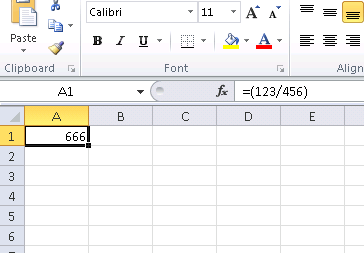
\includegraphics[scale=\NormalScale]{digging_into_code/Excel_prank.png}
\caption{\RU{Пранк сработал}\EN{The practical joke worked}}
\end{figure}

\RU{Если попробовать ту же версию Excel, только x64, то окажется что там инструкций \FDIV всего 12, 
причем нужная нам\EMDASH{}третья по счету.}
\EN{If we try the same Excel version, but in x64,
we will find only 12 \FDIV instructions there,
and the one we looking for is the third one.}

\begin{lstlisting}
tracer.exe -l:excel.exe bpx=excel.exe!BASE+0x1B7FCC,set(st0,666)
\end{lstlisting}

\myindex{x86!\Instructions!DIVSD}
\RU{Видимо, все дело в том, что много операций деления переменных типов \Tfloat и \Tdouble 
компилятор заменил на SSE-инструкции вроде \TT{DIVSD}, 
коих здесь теперь действительно много (\TT{DIVSD} присутствует в количестве 268 инструкций).}
\EN{It seems that a lot of division operations of \Tfloat and \Tdouble types, were replaced by the compiler with SSE instructions
like \TT{DIVSD} (\TT{DIVSD} is present 268 times in total).}


\chapter{\IFRU{Подозрительные паттерны кода}{Suspicious code patterns}}

\section{\IFRU{Инструкции XOR}{XOR instructions}}
\index{x86!\Instructions!XOR}

\IFRU{Инструкции вроде}{instructions like} \TT{XOR op, op} (\IFRU{например}{for example}, \TT{XOR EAX, EAX}) 
\IFRU{обычно используются для обнуления регистра,
однако, если операнды разные, то применяется операция именно}{are usually used for setting register value
to zero, but if operands are different,} \IT{\IFRU{исключающего или}{exclusive or}}\EN{ operation
is executed}.
\IFRU{Эта операция очень редко применяется в обычном программировании, но применяется очень часто в криптографии,
включая любительскую}{This operation is rare in common programming, but used often in cryptography,
including amateur}.
\IFRU{Особенно подозрительно, если второй операнд это большое число}{Especially suspicious case if the
second operand is big number}.
\IFRU{Это может указывать на шифрование, вычисление контрольной суммы, итд}
{This may points to encrypting/decrypting, checksum computing, etc}.\\
\\
\IFRU{Одно из исключений из этого наблюдения о котором стоит сказать, то, что генерация и проверка значения ``канарейки''
(\ref{subsec:BO_protection}) часто происходит используя инструкцию \XOR}
{One exception to this observation worth to note is ``canary'' (\ref{subsec:BO_protection}) generation and checking is often done using \XOR
instruction}. \\
\\
\index{AWK}
\IFRU{Этот AWK-скрипт можно использовать для обработки листингов (.lst) созданных \IDA{}}
{This AWK script can be used for processing \IDA{} listing (.lst) files}:

\begin{lstlisting}
gawk -e '$2=="xor" { tmp=substr($3, 0, length($3)-1); if (tmp!=$4) if($4!="esp") if ($4!="ebp") { print $1, $2, tmp, ",", $4 } }' filename.lst
\end{lstlisting}

\IFRU{Нельзя также забывать,
что если использовать подобный скрипт, то, возможно, он захватит и неверно дизассемблированный
код}{It is also worth to note that such script may also capture incorrectly disassembled code} 
(\ref{sec:incorrectly_disasmed_code}).

\section{\IFRU{Вручную написанный код на ассемблере}{Hand-written assembly code}}

\index{Function prologue}
\index{Function epilogue}
\index{x86!\Instructions!LOOP}
\index{x86!\Instructions!RCL}
\IFRU{Современные компиляторы не генерируют инструкции \TT{LOOP} и \TT{RCL}. 
С другой стороны, эти инструкции хорошо знакомы кодерам, предпочитающим писать прямо на ассемблере. 
Подобные инструкции отмечены как (M) в списке инструкций в приложении: \ref{sec:x86_instructions}.
Если такие инструкции встретились, можно сказать с какой-то вероятностью, что этот фрагмент кода написан вручную.}
{Modern compilers do not emit \TT{LOOP} and \TT{RCL} instructions.
On the other hand, these instructions are well-known to coders who like to code in straight assembly language.
If you spot these, it can be said, with a high probability, this fragment of code is hand-written.
Such instructions are marked as (M) in the instructions list in appendix: \ref{sec:x86_instructions}.}\\
\\
\IFRU{Также, пролог/эпилог функции обычно не встречается в ассемблерном коде, написанном вручную.}
{Also function prologue/epilogue is not commonly present in hand-written assembly copy.}\\
\\
\IFRU{Как правило, в вручную написанном коде, нет никакого четкого метода передачи аргументов в 
функцию}
{Commonly there is no fixed system in passing arguments into functions in the hand-written
code}.\\
\\
\IFRU{Пример из ядра}{Example from} Windows 2003\EN{ kernel} 
(\RU{файл }ntoskrnl.exe\EN{ file}):

\begin{lstlisting}
MultiplyTest proc near               ; CODE XREF: Get386Stepping
             xor     cx, cx
loc_620555:                          ; CODE XREF: MultiplyTest+E
             push    cx
             call    Multiply
             pop     cx
             jb      short locret_620563
             loop    loc_620555
             clc
locret_620563:                       ; CODE XREF: MultiplyTest+C
             retn
MultiplyTest endp

Multiply     proc near               ; CODE XREF: MultiplyTest+5
             mov     ecx, 81h
             mov     eax, 417A000h
             mul     ecx
             cmp     edx, 2
             stc
             jnz     short locret_62057F
             cmp     eax, 0FE7A000h
             stc
             jnz     short locret_62057F
             clc
locret_62057F:                       ; CODE XREF: Multiply+10
                                     ; Multiply+18
             retn
Multiply     endp
\end{lstlisting}

\IFRU{Действительно, если заглянуть в исходные коды}{Indeed, if we look into} 
\ac{WRK} v1.2\IFRU{, данный код можно найти в файле}{ source code, this code
can be found easily in the file} 
\IT{WRK-v1.2\textbackslash{}base\textbackslash{}ntos\textbackslash{}ke\textbackslash{}i386\textbackslash{}cpu.asm}.


\section{\IFRU{Использование magic numbers для трассировки}{Using magic numbers while tracing}}

\IFRU{Нередко бывает нужно узнать, как используется то или иное значение прочитанное из файла либо взятое из пакета
принятого по сети. Часто, ручное слежение за нужной переменной это трудный процесс. Один из простых методов (хотя и не
полностью надежный на 100\%) это использование вашей собственной \IT{magic number}.}
{Often, main goal is to get to know, how a value was read from file, or received via network, being used. 
Often, manual tracing of a value is very labouring task. One of the simple methods (however, not 100\% reliable) 
is to use your own \IT{magic number}.}

\IFRU{Это чем-то напоминает компьютерную томографию: пациенту перед сканированием вводят в кровь 
рентгеноконтрастный препарат, хорошо отсвечивающий в рентгеновских лучах. Известно как кровь нормального человека
расходится, например, по почкам, и если в этой крови будет препарат, то при томографии будет хорошо видно,
достаточно ли хорошо кровь расходится по почкам и нет ли там камней, например, и прочих образований.}
{This resembling X-ray computed tomography is some sense: radiocontrast agent is often injected into patient's blood,
which is used for improving visibility of internal structures in X-rays. For example, it is well known how blood of healthy man/woman
percolates in kidneys and if agent is in blood, it will be easily seen on tomography, how good and normal blood was percolating,
are there any stones or tumors.}

\IFRU{Мы можем взять 32-битное число вроде \IT{0x0badf00d}, либо чью-то дату рождения вроде \IT{0x11101979} 
и записать это, занимающее 4 байта число, в какое-либо место файла используемого исследуемой нами программой.}
{We can take a 32-bit number like \IT{0x0badf00d}, or someone's birth date like \IT{0x11101979}
and to write this, 4 byte holding number, to some point in file used by the program we investigate.}

\index{\GrepUsage}
\IFRU{Затем, при трассировки этой программы, в том числе, при помощи \tracer в режиме 
\IT{code coverage}, а затем при помощи
\IT{grep} или простого поиска по текстовому файлу с результатами трассировки, мы можем легко увидеть, в каких местах кода использовалось 
это значение, и как.}
{Then, while tracing this program, with \tracer in the \IT{code coverage} mode, and then, with the help of \IT{grep}
or just by searching in the text file (of tracing results), we can easily see, where the value was used and how.}

\IFRU{Пример результата работы \tracer в режиме \IT{cc}, к которому легко применить утилиту \IT{grep}}{Example 
of \IT{grepable} \tracer results in the \IT{cc} mode}:

\begin{lstlisting}
0x150bf66 (_kziaia+0x14), e=       1 [MOV EBX, [EBP+8]] [EBP+8]=0xf59c934 
0x150bf69 (_kziaia+0x17), e=       1 [MOV EDX, [69AEB08h]] [69AEB08h]=0 
0x150bf6f (_kziaia+0x1d), e=       1 [FS: MOV EAX, [2Ch]] 
0x150bf75 (_kziaia+0x23), e=       1 [MOV ECX, [EAX+EDX*4]] [EAX+EDX*4]=0xf1ac360 
0x150bf78 (_kziaia+0x26), e=       1 [MOV [EBP-4], ECX] ECX=0xf1ac360 
\end{lstlisting}

\IFRU{Это справедливо также и для сетевых пакетов.
Важно только чтобы наш \IT{magic number} был как можно более уникален и не присутствовал в самом коде.}
{This can be used for network packets as well.
It is important to be unique for \IT{magic number} and not to be present in the program's code.}

\newcommand{\DOSBOXURL}{\url{http://blog.yurichev.com/node/55}}

\index{DosBox}
\IFRU{Помимо \tracer, такой эмулятор MS-DOS как DosBox, в режиме heavydebug, может писать в отчет информацию обо всех
состояниях регистра на каждом шаге исполнения программы\footnote{См.также мой пост в блоге об этой возможности в 
DosBox: \DOSBOXURL{}}, так что этот метод может пригодиться и я для исследования программ под DOS.}{Aside of 
\tracer, DosBox (MS-DOS emulator) in heavydebug mode,
is able to write information about all register's states for each executed instruction of program to plain text file\footnote{See also my 
blog post about this DosBox feature: \DOSBOXURL{}}, so this method may be useful for DOS programs as well.}



\section{\IFRU{Старые методы, тем не менее, интересные}{Old-school methods, nevertheless, interesting to know}}

\subsection{\IFRU{Сравнение ``снимков'' памяти}{Memory ``snapshots'' comparing}}

\IFRU{Метод простого сравнения двух снимков памяти для поиска изменений часто применялся для взлома игр 
на 8-битных компьютерах и взлома файлов с записанными рекордными очками.}
{The method of simple two memory snapshots comparing in order to see changes, was often used to hack
8-bit computer games and hacking ``high score'' files.}

\IFRU{К примеру, если вы имеете загруженную игру на 8-битном компьютере (где самой памяти не очень много, но игра
занимает еще меньше), и вы знаете что сейчас у вас, условно, 100 пуль, вы можете сделать ``снимок'' всей
памяти и сохранить где-то. Затем просто стреляете куда угодно, у вас станет 99 пуль, сделать второй ``снимок'',
и затем сравнить эти два снимка: где-то наверняка должен быть байт, который в начале был 100, а затем стал 99.}
{For example, if you got some loaded game on 8-bit computer (it's not much memory on these, but game is usually
consumes even less memory) and you know that you have now, let's say, 100 bullets, you can do a ``snapshot''
of all memory and save it to some place. Then shoot somewhere, bullet count now 99, do second ``snapshot''
and then compare both: somewhere should be a byte which was 100 in the beginning and now it's 99.}
\IFRU{Если учесть что игры на тех маломощных домашних компьютерах обычно были написанны на ассемблере и подобные
переменные там были глобальные, то можно с уверенностью сказать, какой адрес в памяти всегда отвечает за количество
пуль. Если поискать в дизассемблированном коде игры все обращения по этому адресу, несложно найти код,
отвечающий за уменьшение пуль и записать туда инструкцию \NOP\footnote{``no operation'', холостая инструкция} 
или несколько \NOP-в, так мы получим игру в которой у игрока всегда будет 100 пуль, например.}
{Considering a fact that these 8-bit games were often written in assembler and such variables were global,
it can be said for sure, which address in memory holding bullets count. If to search all references to that
address in disassembled game code, it's not very hard to find a piece of code decrementing bullets count,
write \NOP instruction\footnote{``no operation'', idle operation} there, or couple of \NOP{}-s, 
we'll have a game with 100 (for example) bullets forever.}
\IFRU{А так как игры на тех домашних 8-битных 
компьютерах всегда загружались по одним и тем же адресам, и версий одной игры редко когда было больше одной,
то геймеры-энтузиасты знали, по какому адресу (используя инструкцию языка BASIC \IT{POKE}\footnote{инструкция языка BASIC записывающая байт по определенному адресу}) что записать после загрузки
игры, чтобы хакнуть её. Это привело к появлению списков ``читов'' состоящих из инструкций \IT{POKE}, публикуемых
в журналах посвященным 8-битным играм. См.также:}{Games on these 8-bit computers was usually loaded on the same
address, also, there were no much different versions of each game (usually, just one version all have),
enthusiastic gamers knew, which byte should be written (using BASIC instruction \IT{POKE}\footnote{BASIC language instruction writting byte on specific address}) to which address in
order to hack it. This led to ``cheat'' lists containing of \IT{POKE} instructions published in magazines related to
8-bit games. See also:} \url{http://en.wikipedia.org/wiki/PEEK\_and\_POKE}.

\IFRU{Точно также легко модифицировать файлы с сохраненными рекордами, кто сколько очков набрал, впрочем, это может
сработать не только с 8-битными играми. Нужно заметить, какой у вас сейчас рекорд и где-то сохранить файл
с очками. Затем, когда очков станет другое количество, просто сравнить два файла, можно даже
DOS-утилитой FC\footnote{утилита MS-DOS для сравнения двух файлов побайтово} (файлы рекордов, часто, бинарные).}
{The same story about modifying ``high score'' files, this may work not only with 8-bit games. Let's notice 
your score count and save the file somewhere. When ``high score'' count will be different, just compare two files,
it can be even done with DOS-utility FC\footnote{MS-DOS utility for binary files comparing} (``high score'' files
are often in binary form).}
\IFRU{Где-то будут отличаться несколько байт, и легко будет увидеть, какие именно отвечают за количество очков. 
Впрочем, разработчики игр осведомлены о таких хитростях и могут защититься от этого.}
{There will be some place where couple of bytes will be different and it will be easy to see which ones are
holding score number.
However, game developers are aware of such tricks and may protect against it.}

% FIXME: пример с какой-то простой игрушкой?




\chapter{\IFRU{Задачи}{Tasks}}

\IFRU{Почти для всех задач, если не указано иное, два вопроса:}
{There are two questions almost for every task, if otherwise is not specified:}

1) \IFRU{Что делает эта функция? Ответ должен состоять из одной фразы.}
{What this function does? Answer in one-sentence form.}

2) \IFRU{Перепишите эту функцию на \CCpp}{Rewrite this function into \CCpp}.

\IFRU{Подсказки и ответы собраны в приложении к этой книге.}{Hints and solutions are in the appendix of
this book.}

\section{\IFRU{Легкий уровень}{Easy level}}

\subsection{\Task 1.1}

\IFRU{Это стандартная функция из библиотек Си. Исходник взят из OpenWatcom. Скомпилировано в MSVC 2010.}
{This is standard C library function. Source code taken from OpenWatcom. Compiled in MSVC 2010.}

\lstinputlisting{tasks/tasks_1_1_msvc.asm}

\IFRU{Это он же скомпилирован при помощи GCC 4.4.1 с опцией \Othree (максимальная оптимизация)}
{It is the same code compiled by GCC 4.4.1 with \Othree option (maximum optimization)}:

\lstinputlisting{tasks/tasks_1_1_gcc.asm}

\subsection{\Task 1.2}

\IFRU{Это также стандартная функция из библиотек Си. Исходник взят из OpenWatcom и немного переделан. 
Скомпилировано в MSVC 2010 с флагом (\Ox).}
{This is also standard C library function. Source code is taken from OpenWatcom and modified slightly.
Compiled in MSVC 2010 with \Ox optimization flag.}

\IFRU{Эта функция использует стандартные функции Си:}
{This function also use these standard C functions:} isspace() \AndENRU isdigit().

\lstinputlisting{tasks/tasks_1_2_msvc.asm}

\IFRU{То же скомпилировано в GCC 4.4.1. Задача немного усложняется тем, что GCC представил isspace() и isdigit() 
как inline-функции и вставил их тела прямо в код.}
{Same code compiled in GCC 4.4.1. This task is sligthly harder since GCC compiled isspace() and isdigit()
functions as inline-functions and inserted their bodies right into the code.}

\lstinputlisting{tasks/tasks_1_2_gcc.asm}

\subsection{\Task 1.3}

\IFRU{Это также стандартная функция из библиотек Си, а вернее, две функции, работающие в паре. 
Исходник взят из MSVC 2010 и немного переделан.}
{This is standard C function too, actually, two functions working in pair.
Source code taken from MSVC 2010 and modified sligthly.}

\IFRU{Суть переделки в том, что эта функция может корректно работать в мульти-тредовой среде, 
а я, для упрощения (или запутывания) убрал поддержку этого.}
{The matter of modification is that this function can work properly in multi-threaded environment,
and I removed its support for simplification (or for confusion).}

\IFRU{Скомпилировано в MSVC 2010 с флагом (\Ox)}{Compiled in MSVC 2010 with \Ox flag}.

\lstinputlisting{tasks/tasks_1_3_msvc.asm}

\IFRU{То же скомпилировано при помощи GCC 4.4.1}{Same code compiled in GCC 4.4.1}:

\lstinputlisting{tasks/tasks_1_3_gcc.asm}

\subsection{\Task 1.4}

\IFRU{Это стандартная функция из библиотек Си. Исходник взят из MSVC 2010. Скомпилировано в MSVC 2010 с флагом \Ox.}
{This is standard C library function. Source code taken from MSVC 2010. Compiled in MSVC 2010 with \Ox flag.}

\lstinputlisting{tasks/tasks_1_4_msvc.asm}

\IFRU{То же скомпилировано при помощи GCC 4.4.1}
{Same code compiled in GCC 4.4.1}:

\lstinputlisting{tasks/tasks_1_4_gcc.asm}

\subsection{\Task 1.5}

\IFRU{Задача, скорее, на эрудицию, нежели на чтение кода.}
{This task is rather on knowledge than on reading code.}

\IFRU{Функция взята из OpenWatcom. Скомпилировано в MSVC 2010 с флагом \Ox.}
{The function is taken from OpenWatcom. Compiled in MSVC 2010 with \Ox flag.}

\lstinputlisting{tasks/tasks_1_5_msvc.asm}

\subsection{\Task 1.6}

\IFRU{Скомпилировано в MSVC 2010 с ключом \Ox.}
{Compiled in MSVC 2010 with \Ox option.}

\lstinputlisting{tasks/tasks_1_6_msvc.asm}

\subsection{\Task 1.7}

\IFRU{Это взята функция из ядра Linux 2.6.}{This function is taken from Linux 2.6 kernel.}

\IFRU{Скомпилировано в MSVC 2010 с опцией \Ox:}{Compiled in MSVC 2010 with \Ox option:}

\lstinputlisting{tasks/tasks_1_7_msvc.asm}

\subsection{\Task 1.8}

\IFRU{Скомпилировано в MSVC 2010 с опцией \TT{/O1}\footnote{/O1: оптимизация по размеру кода}:}
{Compiled in MSVC 2010 with \TT{/O1} option\footnote{/O1: minimize space}:}

\lstinputlisting{tasks/tasks_1_8_msvc.asm}

\subsection{\Task 1.9}

\IFRU{Скомпилировано в MSVC 2010 с опцией \TT{/O1}:}
{Compiled in MSVC 2010 with \TT{/O1} option:}

\lstinputlisting{tasks/tasks_1_9_msvc.asm}

\subsection{\Task 1.10}

\IFRU{Если это скомпилировать и запустить, появится некоторое число. Откуда оно берется? 
Откуда оно берется если скомпилировать в MSVC с оптимизациями (\Ox)?}
{If to compile this piece of code and run, some number will be printed. Where it came from?
Where it came from if to compile it in MSVC with optimization (\Ox)?}

\begin{lstlisting}
#include <stdio.h>

int main()
{
	printf ("%d\n");

	return 0;
};
\end{lstlisting}

\section{\IFRU{Средний уровень}{Middle level}}

\subsection{\Task 2.1}

\IFRU{Довольно известный алгоритм, также включен в стандартную библиотеку Си. Исходник взят из glibc 2.11.1. 
Скомпилирован в GCC 4.4.1 с ключом \TT{-Os} (оптимизация по размеру кода). 
Листинг сделан дизассемблером IDA 4.9 из ELF-файла созданным GCC и линкером.}
{Well-known algorithm, also included in standard C library. Source code was taken from glibc 2.11.1.
Compiled in GCC 4.4.1 with \TT{-Os} option (code size optimization).
Listing was done by IDA 4.9 disassembler from ELF-file generated by GCC and linker.}

\IFRU{Для тех кто хочет использовать IDA в процессе изучения, вот здесь лежат .elf и .idb файлы, 
.idb можно открыть при помощи бесплатой IDA 4.9:}
{For those who wants use IDA while learning, here you may find .elf and .idb files,
.idb can be opened with freeware IDA 4.9:}

\url{http://conus.info/RE-tasks/middle/1/}

\lstinputlisting{tasks/tasks_2_1_gcc.asm}

\section{crackme / keygenme}

\IFRU{Несколько моих keygenme\footnote{программа имитирующая защиту вымышленной программы, 
для которой нужно сделать генератор ключей/лицензий.}:}
{Couple of my keygenmes\footnote{program which imitates fictional software protection, 
for which one needs to make a keys/licenses generator}:}

\url{http://crackmes.de/users/yonkie/}



\part{\RU{Инструменты}\EN{Tools}}

\chapter{\RU{Дизассемблер}\EN{Disassembler}}

\section{IDA}

\label{IDA}
\RU{Старая бесплатная версия доступна для скачивания}\EN{Older freeware version is available for downloading}
\footnote{\url{http://www.hex-rays.com/idapro/idadownfreeware.htm}}.

\ShortHotKeyCheatsheet: \ref{sec:IDA_cheatsheet}

\chapter{\RU{Отладчик}\EN{Debugger}}

\section{tracer}

\index{tracer}
\label{tracer}
\RU{Я использую}\EN{I use} \IT{tracer}\footnote{\url{http://yurichev.com/tracer-\LANG.html}}
\RU{вместо отладчика}\EN{instead of debugger}.

\RU{Со временем я отказался использовать отладчик, потому что все что мне нужно от него: это иногда подсмотреть 
какие-либо аргументы какой-либо функции во время исполнения или состояние регистров в определенном месте. 
Каждый раз загружать отладчик для этого это слишком, поэтому я написал очень простую утилиту \IT{tracer}. 
Она консольная, запускается из командной строки, позволяет перехватывать исполнение функций, 
ставить брякпойнты на произвольные места, смотреть состояние регистров, модифицировать их, и так далее.}
\EN{I stopped to use debugger eventually, since all I need from it is to spot a function's arguments while
execution, or registers' state at some point.
To load debugger each time is too much, so I wrote a small utility \IT{tracer}.
It has console-interface, working from command-line, enable us to intercept function execution,
set breakpoints at arbitrary places, spot registers' state, modify it, etc.}

\RU{Но для учебы, очень полезно трассировать код руками в отладчике, наблюдать как меняются значения регистров 
(например, как минимум классический SoftICE, OllyDbg, WinDbg подсвечивают измененные регистры), 
флагов, данные, менять их самому, смотреть реакцию, и т.д.}
\EN{However, as for learning purposes, it is highly advisable to trace code in debugger manually, watch how register's state
changing (e.g. classic SoftICE, OllyDbg, WinDbg highlighting changed registers), flags, data, change them
manually, watch reaction, etc.}

\section{\olly}
\index{\olly}

\RU{Очень популярный отладчик пользовательской среды win32}\EN{Very popular user-mode win32 debugger}:\\
\url{http://www.ollydbg.de/}.

\ShortHotKeyCheatsheet: \label{sec:Olly_cheatsheet}

\section{GDB}
\index{GDB}

\RU{Не очень популярный отладчик у реверсеров, тем не менее, крайне удобный}\EN{Not very popular
debugger among reverse engineers, but very comfortable nevertheless}.
\RU{Некоторые команды}\EN{Some commands}: \ref{sec:GDB_cheatsheet}.

\chapter{\RU{Трассировка системных вызовов}\EN{System calls tracing}}

\label{strace}
\index{strace}
\index{dtruss}
\subsection{strace / dtruss}

\index{syscalls}
\RU{Позволяет показать, какие системные вызовы (syscalls(\ref{syscalls})) прямо сейчас вызывает процесс}
\EN{Will show which system calls (syscalls(\ref{syscalls})) are called by process right now}.
\RU{Например}\EN{For example}:

\begin{lstlisting}
# strace df -h

...

access("/etc/ld.so.nohwcap", F_OK)      = -1 ENOENT (No such file or directory)
open("/lib/i386-linux-gnu/libc.so.6", O_RDONLY|O_CLOEXEC) = 3
read(3, "\177ELF\1\1\1\0\0\0\0\0\0\0\0\0\3\0\3\0\1\0\0\0\220\232\1\0004\0\0\0"..., 512) = 512
fstat64(3, {st_mode=S_IFREG|0755, st_size=1770984, ...}) = 0
mmap2(NULL, 1780508, PROT_READ|PROT_EXEC, MAP_PRIVATE|MAP_DENYWRITE, 3, 0) = 0xb75b3000
\end{lstlisting}

\index{\MacOSX}
\RU{В \MacOSX для этого же имеется dtruss}\EN{\MacOSX has dtruss for the same aim}.

\index{cygwin}
\RU{В Cygwin также есть strace, впрочем, если я верно понял, 
он показывает результаты только для .exe-файлов скомпилированных для среды самого cygwin}
\EN{The Cygwin also has strace, but if I understood correctly, it works only for .exe-files
compiled for cygwin environment itself}.

\chapter{\RU{Декомпиляторы}\EN{Decompilers}}

\RU{Пока существует только один, публично доступный, декомпилятор в Си высокого качества}
\EN{There are only one known, publically available, high-quality decompiler to C code}: Hex-Rays:\\
\url{https://www.hex-rays.com/products/decompiler/}

% TODO Java, .NET, VB, etc

\chapter{\RU{Прочие инструменты}\EN{Other tools}}

\begin{itemize}
\item
Microsoft Visual Studio Express\footnote{\url{http://www.microsoft.com/express/Downloads/}}:
\RU{Усеченная бесплатная версия Visual Studio, пригодная для простых экспериментов}
\EN{Stripped-down free Visual Studio version, convenient for simple experiments}.
Some useful options: \ref{sec:MSVC_options}.

\item
\label{Hiew}
Hiew\footnote{\url{http://www.hiew.ru/}} \RU{для мелкой модификации кода в исполняемых файлах}
\EN{for small modifications of code in binary files}.

\item
\index{binary grep}
binary grep: \RU{небольшая утилита для поиска констант (либо просто последовательности байт)
в большом  кол-ве файлов, включая неисполняемые: \BGREPURL.}
\EN{the small utility for constants searching (or just any byte sequence) in a big pile of files, 
including non-executable: \BGREPURL.}
\end{itemize}



\chapter{\IFRU{Что стоит почитать}{Books/blogs worth reading}}

\section{\IFRU{Книги}{Books}}

\subsection{Windows}

\begin{itemize}
\item
Windows® Internals (Mark E. Russinovich and David A. Solomon with Alex Ionescu)\footnote{\url{http://www.microsoft.com/learning/en/us/book.aspx?ID=12069&locale=en-us}}
\end{itemize}

\subsection{\CCpp}

\begin{itemize}
\item
\IFRU{Стандарт языка Си++}{C++ language standard}: ISO/IEC 14882:2003\footnote{\url{http://www.iso.org/iso/catalogue_detail.htm?csnumber=38110}}
\end{itemize}

\subsection{x86 / x86-64}

\begin{itemize}
\item
\IFRU{Документация от Intel}{Intel manuals}: \url{http://www.intel.com/products/processor/manuals/}
\item
\IFRU{Документация от AMD}{AMD manuals}: \url{http://developer.amd.com/documentation/guides/Pages/default.aspx#manuals}
\end{itemize}

\section{\IFRU{Блоги}{Blogs}}

\subsection{Windows}

\begin{itemize}
\item
\href{http://blogs.msdn.com/oldnewthing/}{Microsoft: Raymond Chen}
\item
\url{http://www.nynaeve.net/}
\end{itemize}



\chapter{\IFRU{Прочее}{Other things}}

\section{\IFRU{Еще примеры}{More examples}}

\begin{itemize}
\item
(eng) \url{http://conus.info/RE-articles/qr9.html}
\item
(eng) \url{http://conus.info/RE-articles/sapgui.html}
\end{itemize}

\section{\IFRU{Аномалии компиляторов}{Compiler's anomalies}}

\IFRU{Intel C++ 10.1 которым скомпилирован Oracle RDBMS 11.2 Linux86, может сгенерировать два \JZ идущих подряд, 
причем на второй \JZ нет ссылки ниоткуда. Второй \JZ таким образом, не имеет никакого смысла.}
{Intel C++ 10.1, which was used for Oracle RDBMS 11.2 Linux86 compilation, may emit two \JZ in row,
and there are no references to the second \JZ. Second \JZ is thus senseless.}

\IFRU{Например, kdli.o из}{For example, kdli.o from} libserver11.a:

\begin{lstlisting}
.text:08114CF1                   loc_8114CF1:                            ; CODE XREF: __PGOSF539_kdlimemSer+89A
.text:08114CF1                                                           ; __PGOSF539_kdlimemSer+3994
.text:08114CF1 8B 45 08                          mov     eax, [ebp+arg_0]
.text:08114CF4 0F B6 50 14                       movzx   edx, byte ptr [eax+14h]
.text:08114CF8 F6 C2 01                          test    dl, 1
.text:08114CFB 0F 85 17 08 00 00                 jnz     loc_8115518
.text:08114D01 85 C9                             test    ecx, ecx
.text:08114D03 0F 84 8A 00 00 00                 jz      loc_8114D93
.text:08114D09 0F 84 09 08 00 00                 jz      loc_8115518
.text:08114D0F 8B 53 08                          mov     edx, [ebx+8]
.text:08114D12 89 55 FC                          mov     [ebp+var_4], edx
.text:08114D15 31 C0                             xor     eax, eax
.text:08114D17 89 45 F4                          mov     [ebp+var_C], eax
.text:08114D1A 50                                push    eax
.text:08114D1B 52                                push    edx
.text:08114D1C E8 03 54 00 00                    call    len2nbytes
.text:08114D21 83 C4 08                          add     esp, 8
\end{lstlisting}

\IFRU{Еще там же:}{From the same code:}

\begin{lstlisting}
.text:0811A2A5                   loc_811A2A5:                            ; CODE XREF: kdliSerLengths+11C
.text:0811A2A5                                                           ; kdliSerLengths+1C1
.text:0811A2A5 8B 7D 08                          mov     edi, [ebp+arg_0]
.text:0811A2A8 8B 7F 10                          mov     edi, [edi+10h]
.text:0811A2AB 0F B6 57 14                       movzx   edx, byte ptr [edi+14h]
.text:0811A2AF F6 C2 01                          test    dl, 1
.text:0811A2B2 75 3E                             jnz     short loc_811A2F2
.text:0811A2B4 83 E0 01                          and     eax, 1
.text:0811A2B7 74 1F                             jz      short loc_811A2D8
.text:0811A2B9 74 37                             jz      short loc_811A2F2
.text:0811A2BB 6A 00                             push    0
.text:0811A2BD FF 71 08                          push    dword ptr [ecx+8]
.text:0811A2C0 E8 5F FE FF FF                    call    len2nbytes
\end{lstlisting}

\IFRU{Возможно, это ошибка его кодегенератора, не выявленная тестами 
(ведь результирующий код и так работает нормально).}
{It's probably code generator bug wasn't found by tests, because, 
resulting code is working correctly anyway.}

% done

\chapter{\IFRU{Ответы на задачи}{Tasks solutions}}

\section{\IFRU{Легкий уровень}{Easy level}}

\subsection{\Task 1.1}

\IFRU{Решение}{Solution}: \TT{toupper()}.

\IFRU{Исходник на Си}{C source code}:

\begin{lstlisting}
char toupper ( char c )
{
    if( c >= 'a' && c <= 'z' ) {
        c = c - 'a' + 'A';
    }
    return( c );
}
\end{lstlisting}

\subsection{\Task 1.2}

\IFRU{Ответ}{Solution}: \TT{atoi()}

\IFRU{Исходник на Си}{C source code}:

\begin{lstlisting}
#include <stdio.h>
#include <string.h>
#include <ctype.h>

int atoi ( const *p )  /* convert ASCII string to integer */
{
    int i;
    char s;

    while( isspace ( *p ) )
        ++p;
    s = *p;
    if( s == '+' || s == '-' )
        ++p;
    i = 0;
    while( isdigit(*p) ) {
        i = i * 10 + *p - '0';
        ++p;
    }
    if( s == '-' )
        i = - i;
    return( i );
}
\end{lstlisting}

\subsection{\Task 1.3}

\IFRU{Ответ}{Solution}: \TT{srand()} / \TT{rand()}.

\IFRU{Исходник на Си}{C source code}:

\begin{lstlisting}
static unsigned int v;

void srand (unsigned int s)
{
        v = s;
}

int rand ()
{
        return( ((v = v * 214013L
            + 2531011L) >> 16) & 0x7fff );
}
\end{lstlisting}

\subsection{\Task 1.4}

\IFRU{Ответ}{Solution}: \TT{strstr()}.

\IFRU{Исходник на Си}{C source code}:

\begin{lstlisting}
char * strstr (
        const char * str1,
        const char * str2
        )
{
        char *cp = (char *) str1;
        char *s1, *s2;

        if ( !*str2 )
            return((char *)str1);

        while (*cp)
        {
                s1 = cp;
                s2 = (char *) str2;

                while ( *s1 && *s2 && !(*s1-*s2) )
                        s1++, s2++;

                if (!*s2)
                        return(cp);

                cp++;
        }

        return(NULL);

}
\end{lstlisting}

\subsection{\Task 1.5}

\IFRU{Подсказка}{Hint} \#1: \IFRU{Не забывайте что}{Keep in mind that} \TT{\_\_v} ~--- 
\IFRU{глобальная переменная}{global variable}.

\IFRU{Подсказка}{Hint} \#2: \IFRU{Эта функция вызывается startup-кодом перед вызовом \main}
{That function is called in startup code, before \main execution}.

\IFRU{Ответ: это проверка на наличие FDIV-ошибки в ранних процессорах Pentium}
{Solution: early Pentium CPU FDIV bug checking}\footnote{\url{http://en.wikipedia.org/wiki/Pentium_FDIV_bug}}.

\IFRU{Исходник на Си}{C source code}:

\begin{lstlisting}
unsigned _v; // _v

enum e {
    PROB_P5_DIV = 0x0001
};

void f( void ) // __verify_pentium_fdiv_bug
{
    /*
        Verify we have got the Pentium FDIV problem.
        The volatiles are to scare the optimizer away.
    */
    volatile double     v1     = 4195835;
    volatile double     v2   = 3145727;

    if( (v1 - (v1/v2)*v2) > 1.0e-8 ) {
        _v |= PROB_P5_DIV;
    }
}
\end{lstlisting}

\subsection{\Task 1.6}

\IFRU{Подсказка: если погуглить применяемую здесь константу, это может помочь.}
{Hint: it might be helpful to google a constant used here.}

\IFRU{Ответ: шифрование алгоритмом TEA}{Solution: TEA encryption algorithm}\footnote{Tiny Encryption Algorithm}.

\IFRU{Исходник на Си}{C source code} (\IFRU{взято с}{taken from} \url{http://en.wikipedia.org/wiki/Tiny_Encryption_Algorithm}):

\begin{lstlisting}
void f (unsigned int* v, unsigned int* k) {
    unsigned int v0=v[0], v1=v[1], sum=0, i;           /* set up */
    unsigned int delta=0x9e3779b9;                     /* a key schedule constant */
    unsigned int k0=k[0], k1=k[1], k2=k[2], k3=k[3];   /* cache key */
    for (i=0; i < 32; i++) {                       /* basic cycle start */
        sum += delta;
        v0 += ((v1<<4) + k0) ^ (v1 + sum) ^ ((v1>>5) + k1);
        v1 += ((v0<<4) + k2) ^ (v0 + sum) ^ ((v0>>5) + k3);  
    }                                              /* end cycle */
    v[0]=v0; v[1]=v1;
}
\end{lstlisting}

\subsection{\Task 1.7}

\IFRU{Подсказка: таблица содержит зараннее вычисленные значения. 
Можно было бы обойтись и без нее, но тогда функция работала бы чуть медленнее.}
{Hint: the table contain pre-calculated values.
It's possible to implement the function without it, but it will work slower, though.}

\IFRU{Ответ: эта функция переставляет все биты во входном 32-битном слове наоборот. 
Это \TT{lib/bitrev.c} из ядра Linux.}
{Solution: this function reverse all bits in input 32-bit integer. 
It's \TT{lib/bitrev.c} from Linux kernel.}

\IFRU{Исходник на Си}{C source code}:

\begin{lstlisting}
const unsigned char byte_rev_table[256] = {
	0x00, 0x80, 0x40, 0xc0, 0x20, 0xa0, 0x60, 0xe0,
	0x10, 0x90, 0x50, 0xd0, 0x30, 0xb0, 0x70, 0xf0,
	0x08, 0x88, 0x48, 0xc8, 0x28, 0xa8, 0x68, 0xe8,
	0x18, 0x98, 0x58, 0xd8, 0x38, 0xb8, 0x78, 0xf8,
	0x04, 0x84, 0x44, 0xc4, 0x24, 0xa4, 0x64, 0xe4,
	0x14, 0x94, 0x54, 0xd4, 0x34, 0xb4, 0x74, 0xf4,
	0x0c, 0x8c, 0x4c, 0xcc, 0x2c, 0xac, 0x6c, 0xec,
	0x1c, 0x9c, 0x5c, 0xdc, 0x3c, 0xbc, 0x7c, 0xfc,
	0x02, 0x82, 0x42, 0xc2, 0x22, 0xa2, 0x62, 0xe2,
	0x12, 0x92, 0x52, 0xd2, 0x32, 0xb2, 0x72, 0xf2,
	0x0a, 0x8a, 0x4a, 0xca, 0x2a, 0xaa, 0x6a, 0xea,
	0x1a, 0x9a, 0x5a, 0xda, 0x3a, 0xba, 0x7a, 0xfa,
	0x06, 0x86, 0x46, 0xc6, 0x26, 0xa6, 0x66, 0xe6,
	0x16, 0x96, 0x56, 0xd6, 0x36, 0xb6, 0x76, 0xf6,
	0x0e, 0x8e, 0x4e, 0xce, 0x2e, 0xae, 0x6e, 0xee,
	0x1e, 0x9e, 0x5e, 0xde, 0x3e, 0xbe, 0x7e, 0xfe,
	0x01, 0x81, 0x41, 0xc1, 0x21, 0xa1, 0x61, 0xe1,
	0x11, 0x91, 0x51, 0xd1, 0x31, 0xb1, 0x71, 0xf1,
	0x09, 0x89, 0x49, 0xc9, 0x29, 0xa9, 0x69, 0xe9,
	0x19, 0x99, 0x59, 0xd9, 0x39, 0xb9, 0x79, 0xf9,
	0x05, 0x85, 0x45, 0xc5, 0x25, 0xa5, 0x65, 0xe5,
	0x15, 0x95, 0x55, 0xd5, 0x35, 0xb5, 0x75, 0xf5,
	0x0d, 0x8d, 0x4d, 0xcd, 0x2d, 0xad, 0x6d, 0xed,
	0x1d, 0x9d, 0x5d, 0xdd, 0x3d, 0xbd, 0x7d, 0xfd,
	0x03, 0x83, 0x43, 0xc3, 0x23, 0xa3, 0x63, 0xe3,
	0x13, 0x93, 0x53, 0xd3, 0x33, 0xb3, 0x73, 0xf3,
	0x0b, 0x8b, 0x4b, 0xcb, 0x2b, 0xab, 0x6b, 0xeb,
	0x1b, 0x9b, 0x5b, 0xdb, 0x3b, 0xbb, 0x7b, 0xfb,
	0x07, 0x87, 0x47, 0xc7, 0x27, 0xa7, 0x67, 0xe7,
	0x17, 0x97, 0x57, 0xd7, 0x37, 0xb7, 0x77, 0xf7,
	0x0f, 0x8f, 0x4f, 0xcf, 0x2f, 0xaf, 0x6f, 0xef,
	0x1f, 0x9f, 0x5f, 0xdf, 0x3f, 0xbf, 0x7f, 0xff,
};

unsigned char bitrev8(unsigned char byte)
{
	return byte_rev_table[byte];
}

unsigned short bitrev16(unsigned short x)
{
	return (bitrev8(x & 0xff) << 8) | bitrev8(x >> 8);
}

/**
 * bitrev32 - reverse the order of bits in a unsigned int value
 * @x: value to be bit-reversed
 */

unsigned int bitrev32(unsigned int x)
{
	return (bitrev16(x & 0xffff) << 16) | bitrev16(x >> 16);
}
\end{lstlisting}

\subsection{\Task 1.8}

\IFRU{Ответ: сложение двух матриц размером 100 на 200 элементов типа \Tdouble.}
{Solution: two 100*200 matrices of type \Tdouble addition.}

\IFRU{Исходник на \CCpp}{\CCpp source code}:

\begin{lstlisting}
#define M    100
#define N    200

void s(double *a, double *b, double *c)
{
  for(int i=0;i<N;i++)
    for(int j=0;j<M;j++)
      *(c+i*M+j)=*(a+i*M+j) + *(b+i*M+j);
};
\end{lstlisting}

\subsection{\Task 1.9}

\IFRU{Ответ: умножение двух матриц размерами 100*200 и 100*300 элементов типа \Tdouble, результат: матрица 100*300.}
{Solution: two matrices (one is 100*200, second is 100*300) of type \Tdouble multiplication, result: 100*300
matrix.}

\IFRU{Исходник на \CCpp}{\CCpp source code}:

\begin{lstlisting}
#define M     100
#define N     200
#define P     300

void m(double *a, double *b, double *c)
{
  for(int i=0;i<M;i++)
    for(int j=0;j<P;j++)
    {
      *(c+i*M+j)=0;
      for (int k=0;k<N;k++) *(c+i*M+j)+=*(a+i*M+j) * *(b+i*M+j);
    }
};
\end{lstlisting}

\section{\IFRU{Средний уровень}{Middle level}}

\subsection{\Task 2.1}

\IFRU{Подсказка \#1: В этом коде есть одна особенность, по которой можно значительно сузить поиск функции в glibc.}
{Hint \#1: The code has one characteristic thing, considering it, it may help narrowing search of right function 
among glibc functions}.

\IFRU{Ответ: особенность ~--- это вызов callback-функции}{Solution: characteristic ~--- is callback-function
calling}~\ref{sec:pointerstofunctions}, 
\IFRU{указатель на которую передается в четвертом аргументе}{pointer to which is passed in 4th
argument}. \IFRU{Это}{It's} \TT{quicksort()}.

\IFRU{Исходник на Си:}{C source code:}

\lstinputlisting{tasks_answers/tasks_2_1.c}



\end{document}
